\documentclass[10pt,a4paper]{article}

\usepackage[utf8]{inputenc}		% Configuro la codificación
\input{.command.tex}
% En el siguiente archivo se configuran las variables del trabajo práctico
%% \providecommand es similar a \newcommnad, salvo que el primero ante un 
%% conflicto en la compilación, es ignorado.

% Al comienzo de un TP se debe modificar los argumentos de los comandos

\providecommand{\myTitle}{EJERCICIO PRÁCTICO}
\providecommand{\mySubtitle}{Simulación de Filtro de Kalman}

\providecommand{\mySubject}{Procesamiento de Señales II (86.51)}
\providecommand{\myKeywords}{UBA, Ingeniería, PS2}

\providecommand{\myAuthorSurname}{Manso}
\providecommand{\myTimePeriod}{Año 2018 - 2\textsuperscript{do} Cuatrimestre}

% No es necesario modificar este %%%%%%%%%%%%%%
\providecommand{\myHeaderLogo}{header_fiuba}
%%%%%%%%%%%%%%%%%%%%%%%%%%%%%%%%%%%%%%%%%%%%%%%%

% Si se utilizan listings, definir el lenguaje aquí
\providecommand{\myLanguage}{matlab}

% Crear los integrantes del TP con el comando \PutMember donde
%%		1) Apellido, Nombre
%%		2) Número de Padrón
%%		3) E-Mail
\providecommand{\MembersOnCover}[0]
{		
		\PutMember{Manso, Juan} {96133} {juanmanso@gmail.com}
}

\providecommand{\myGroupNumber}{11}


\Pagebreakfalse		% Setea si hay un salto de página en la carátula
\Indexfalse
\Siunitxtrue			% Si quiero utilizar el paquete, \siunixtrue. Si no \siunixfalse
\Todonotestrue		% Habilita/Deshabilita las To-Do Notes y las funciones \unsure, \change, \info, \improvement y \thiswillnotshow.
\Listingstrue
\Keywordsfalse
\Putgroupfalse		% Habilita/Deshabilita el \myGroup en los headers
\Videofalse
				% Archivo con los comandos globales como Título y autores
%Preambulo para articulo científico de LaTeX

\usepackage[a4paper,left=3cm,right=3cm,bottom=3.5cm,top=3.5cm]{geometry} 	% Configuro la geometría del papel
%\usepackage{microtype}								% Mejora el "spacing" de las palabras
\usepackage[spanish]{babel} 							% Compatibilizo los signos del español
	\addto\captionsspanish{\renewcommand{\tablename}{Tabla}}		%% Redefino nombres preestablecidos por Babel
	\addto\captionsspanish{\renewcommand{\listtablename}{Índice de tablas}}	%% y así en vez de Cuadro dirá Tabla.
\usepackage{amsmath, amsfonts, amssymb}						% Entornos matemáticos, fuentes y símbolos
\usepackage{graphicx}								% Necesario para insertar figuras
\usepackage{fancyhdr}								% Para manipular headers y footers
\usepackage[usenames,dvipsnames]{color}						% \color{color deseado} {lo que querés que tenga color}
\usepackage{subcaption}								% Permite captions del tipo 1a, 1b
\usepackage{multirow}								% Para tablas
\usepackage{float}

% Para video
\ifVideo
	\usepackage{media9}
	\addmediapath{./../reportes/}
\fi

%\usepackage{times}
%\usepackage{mathtools}
%\usepackage{upgreek} % letras griegas sin cursiva
%\usepackage{cancel}
\usepackage{rotating}
\usepackage{tikz}
\usepackage{pgfplots}
%	\pgfplotsset{compat=1.12}
	\usetikzlibrary{plotmarks}% matlab2tikz
\usepackage{grffile}% matlab2tikz 
	\usetikzlibrary{calc,patterns,decorations.pathmorphing,decorations.markings}

\ifListings
	\usepackage{listings}

	\providecommand{\lstinputpath}[1]{\lstset{inputpath=#1}}

%	\input{.lst_default.tex}
	\input{.lst_matlab.tex}
%	\input{.lst_c.tex}
%	\input{.lst_c++.tex}
	
% 	\input{.lst_pseudocode.tex}


\fi

\ifSiunitx
\usepackage{siunitx}											% Unidades: \SI {cantidad} {\unidad} (necesita texlive-science)
	\sisetup{load-configurations = abbreviations}							% Habilita poner \cm en vez de \centi\metre
	\sisetup{output-decimal-marker = {,}}									% Cambia los puntos decimales por comas
	\sisetup{per-mode = fraction}											% Pone las unidades como fracción
	\sisetup{quotient-mode = fraction}										
\fi


\ifTodonotes
\usepackage{xargs}
\usepackage[colorinlistoftodos,prependcaption,textsize=tiny]{todonotes}


	\newcommandx{\unsure}[2][1=]{\todo[linecolor=red,backgroundcolor=red!25,bordercolor=red,#1]{#2}}
	\newcommandx{\Juan}[2][1=]{\todo[linecolor=blue,backgroundcolor=blue!25,bordercolor=blue,#1]{#2}}
	\newcommandx{\Mati}[2][1=]{\todo[linecolor=green,backgroundcolor=green!25,bordercolor=green,#1]{#2}} % OliveGreen
	\newcommandx{\Emi}[2][1=]{\todo[linecolor=Plum,backgroundcolor=Plum!25,bordercolor=Plum,#1]{#2}}
	\newcommandx{\thiswillnotshow}[2][1=]{\todo[disable,#1]{#2}}
\fi


\usepackage{booktabs}														% Permite hacer tablas sin separadores en el medio
\usepackage{placeins}														
		\let\Oldsection\section												%% Permite que los flotantes (como figuras) no aparescan
	\renewcommand{\section}{\FloatBarrier\Oldsection}						%% antes o después de su sección correspondiente.
		\let\Oldsubsection\subsection
	\renewcommand{\subsection}{\FloatBarrier\Oldsubsection}		
		\let\Oldsubsubsection\subsubsection
	\renewcommand{\subsubsection}{\FloatBarrier\Oldsubsubsection}
\usepackage{hyperref}														% Debe ser agregado al final del preambulo

\hypersetup
{    bookmarks=true,         % show bookmarks bar?
     unicode=false,          % non-Latin characters in Acrobat’s bookmarks
     pdftoolbar=true,        % show Acrobat’s toolbar?
     pdfmenubar=true,        % show Acrobat’s menu?
     pdffitwindow=false,     % window fit to page when opened
     pdftitle={\myTitle},    		 % title
     pdfauthor={\myAuthorSurname},   % author
	 pdfcreator={\myAuthorSurname},	 % creator = author
     pdfsubject={\mySubject},		 % subject of the document
     pdfkeywords={\myKeywords},
     colorlinks=true,        % false: boxed links; true: colored links
     linkcolor=black,        % color of internal links (change box color with linkbordercolor)
     citecolor=black,        % color of links to bibliography
     filecolor=magenta,      % color of file links
     urlcolor=cyan           % color of external links
}

%Configuro la pagina con los encabezaos y pies de paginas
\pagestyle{fancy}										% Para agregar encabezados y pie de paginas	
\lhead{\mySubject}										% Encabezado izquierdo
\rhead{\includegraphics[scale=0.15]{\myHeaderLogo}} 	% Encabezado derecho (logo de la FIUBA)	
\ifPutgroup
\chead{\texttt{Grupo Nº\myGroupNumber} }%\\ \textit{\footnotesize{\myTimePeriod}}}
\fi				

%% Este archivo contiene las funciones auxiliares para escribir en LaTeX
%% Dichas funciones resuelven la sintaxis de generar figuras, por ejemplo,
%% dejando el código más compacto y facilitando la corrección del mismo.



% Comando para graficar eps. 1er arg, escala. 2do, ruta. 3ro, caption. 4to, label.
\providecommand{\HgraficarEPS}[4]{
			\begin{figure}[h!]
				\centering
					\scalebox{#1}{\input{#2}}
					\caption{#3}
					\label{#4}
			\end{figure}

}

\providecommand{\HgraficarPNG}[4]{
			\begin{figure}[h!]
				\centering
					\includegraphics[scale=#1]{#2}
					\caption{#3}
					\label{#4}
			\end{figure}

}


% Comando para graficar eps en el lugar previsto.
\providecommand{\graficarEPS}[4]{
			\begin{figure}[h]
				\centering
					\scalebox{#1}{\input{#2}}
					\caption{#3}
					\label{#4}
			\end{figure}

}

\providecommand{\graficarPNG}[4]{
			\begin{figure}[h]
				\centering
					\includegraphics[scale=#1]{#2}
					\caption{#3}
					\label{#4}
			\end{figure}

}

\providecommand{\underuparrow}[2]{\underset{\underset{#2} \uparrow} #1 }

\providecommand{\cltext}[2]{\color{#1}{\huge{#2}}}

\providecommand{\cstext}[2]{\color{#1}{\large{#2}}}

\providecommand{\vect}[1]{\boldsymbol{#1}}
\providecommand{\dvect}[1]{\dot{\boldsymbol{#1}}}
		% Se proveen un conjunto de funciones extras

% Defino el path de los includegraphics
\graphicspath{{./Figuras/}}		% Directorio que contiene los graficos

% Defino el path para los input de .tex y de .eps
\makeatletter
\def\input@path{{./Figuras/}{./Secciones/}{./Cover_page/}}
\makeatother

% Defino el path del listings
\ifListings
%% Cambiar el nombre de la carpeta si se utilizan Listings
	\lstinputpath{{../Octave/}}
\fi

\definecolor{myred}{rgb}{0.5,0,0}
\definecolor{mygreen}{rgb}{0,0.5,0}



\begin{document}
		% Carátula (formal o simple,_formal o _simple respectivamente) con Resumen
		% incluido e Índice (si es necesario configurar en config.tex) del informe
		

% Configuro la carátula


		\title{{\Large{\textbf{\myTitle}}} \\
				\vspace{0.4cm}
				\normalsize\underline{\textbf{\mySubtitle}} \\
		\author{\small{\textsc{\mySubject}}}}
		\date{\small{\myTimePeriod}}
	\maketitle


\ifPutgroup
	\begin{tabbing}
\hspace{6.7cm}\=\+\texttt{Grupo Nº\myGroupNumber}\hspace{5cm}\=
	\end{tabbing}
\fi
	\begin{tabbing}

		\hspace{2cm} \MembersHeader
		
		\newline \vspace{1cm}
		\MembersOnCover

	\end{tabbing}

%	\begin{abstract}
%		% Ejemplo de Resumen
%% MANTENER EL NOMBRE %%
El presente trabajo tiene como objetivo ejercitar simulaciones de filtro de Kalman.

%	\end{abstract}	



\ifKeywords
	\begin{center}
		\emph{Palabras Clave: \myKeywords}
	\end{center}
\fi



\ifPagebreak
	\pagebreak
\fi
	\ifIndex
		\tableofcontents
%		\listoffigures
%		\listoftables
	\fi

\ifPagebreak
	\pagebreak
\fi




	\setcounter{page}{1}

	%\part{Enunciado}\label{sec:enunciado}
	\section{Enunciado}
		
	Se considera un vehículo que se desplaza definiendo una trayectoria tal que la posición en cada instante resulta $\vect{p}(t)$, con una velocidad $\vect{v}(t)$ y una aceleración $\vect{a}(t)$, definidas en un plano de coordenadas $[x,y]$ de acuerdo a:
	\begin{equation*}
		\vect{p}(t) = \begin{bmatrix} p_x(t) \\[0.3em] p_y(t) \end{bmatrix} \qquad%
		\vect{v}(t) = \begin{bmatrix} v_x(t) \\[0.3em] v_y(t) \end{bmatrix} \qquad%
		\vect{a}(t) = \begin{bmatrix} a_x(t) \\[0.3em] a_y(t) \end{bmatrix}% 
	\end{equation*}

	Suponiendo que la dinámica de movimiento satisface las siguientes ecuaciones:
	\begin{equation}
		\begin{cases}
			\vect{\dot{p}}(t) = \vect{v}(t)\\
			\vect{\dot{v}}(t) = \vect{a}(t)\\
			\vect{\dot{a}}(t) = 0
		\end{cases}
		\label{eq:dinamica_enun}
	\end{equation}



	\section{Ejercicio 1 \\ Modelo En Variables De Estado}\label{sec:ej1}
		\subsection{Inciso a}

	\graficarEPS{0.6}{bloques}{Diagrama en bloques del modelo.}{fig:bloques}
	Se define la variable de estado asociada a las ecuaciones de movimiento continuo como:
		\begin{equation*}
			\vect{x}(t) = \begin{bmatrix} \vect{p}(t) \\[0.3em] \vect{v}(t) \\[0.3em] \vect{a}(t) \end{bmatrix} \qquad%
			\dot{\vect{x}}(t) = \begin{bmatrix} \dot{\vect{p}}(t) \\[0.3em] \dot{\vect{v}}(t) \\[0.3em] \dot{\vect{a}}(t) \end{bmatrix}
		\end{equation*}

	Así el modelo resulta:
		\begin{equation*}
			\Sigma:
			\begin{cases}
				\dvect{x}(t) = A\: \vect{x}(t) + B \: \vect{\xi}(t) \\
				\vect{y}(t) = C\: \vect{x}(t) + \vect{\eta}(t)
			\end{cases}
		\end{equation*}
	donde $\vect{\xi}(t)$ es el ruido de proceso y $\vect{\eta}(t)$ el ruido de medición. La matriz $A$ contiene la información de la dinámica del sistema. A partir de las ecuaciones del sistema representado en \eqref{eq:dinamica_enun} se obtiene la matriz de estados como:
	\unsure{Preguntar cuánto tengo que definir y etc.}

		\begin{equation*}
			A(t) = \begin{bmatrix} I & IT & I\frac{T^2}{2} \\[0.3em] 0 & I & IT \\[0.3em] 0 & 0 & I \end{bmatrix}
		\end{equation*}


\subsection{Inciso b}

	\begin{lstlisting}
config_m;

datos_str = load('datos.mat');

Acel = datos_str.Acel;
Tiempo = datos_str.tiempo;
Pos = datos_str.Pos;
Vel = datos_str.Vel;

dim = 2;			% Se considera sólo x e y
tipos_variables = 3;		% Posición, Velocidad, Aceleración
cant_mediciones = length(Pos);
cant_estados = tipos_variables * dim;



% Datos
var_xip = 3e-4;
var_xiv = 2e-3;
var_xia = 1e-2;

%%%
T = Tiempo(2:end)-Tiempo(1:end-1);	
T = 1;					% Suponiendo equiespaciado

% Variable de estado X = [P;V;A]
I = eye(dim);
Ad =[I		I.*T	(T.^2)/2.*I;
     I*0	I	T.*I;
     I*0	I*0	I;];

% Covarianza del ruido de proceso
Qd = diag([ones(1,dim)*var_xip, ones(1,dim)*var_xiv,ones(1,dim)*var_xia]);
	\end{lstlisting}
% $Q_d=\begin{bmatrix} \sigma^2_{\xi_{px}} &&&&&\\[0.3em] &\sigma^2_{\xi_{py}}&&&&\\[0.3em] &&\sigma^2_{\xi_{vx}}&&&\\[0.3em] &&&\sigma^2_{\xi_{vy}}&&\\[0.3em] &&&&\sigma^2_{\xi_{ax}}&\\[0.3em] &&&&&\sigma^2_{\xi_{ay}}\end{bmatrix}$






	
		

		
	\section{Ejercicio 2 \\ Estimación De lL Trayectoria Con Distintas Mediciones}\label{sec:ej2}
		
	El algoritmo de Kalman se basa en poder estimar el vector de estados a partir de la dinámica del sistema y las mediciones. Para la definición del algoritmo utilizaremos la siguiente notación. Llamaremos:
	
	\begin{equation*}
		\vect{x_{k/k - 1}}
	\end{equation*}
	
	A la mejor estimación de el vector de estados utilizando información hasta el instante $k - 1$. Es decir se trata de una predicción. Llamaremos a la matriz de covarianza del error de dicha estimacion:
	
	\begin{equation*}
		\vect{P_{k/k - 1}}
	\end{equation*}
	
	Por otro lado llamaremos a:
	
	\begin{equation*}
		\vect{x_{k/k}}
	\end{equation*}
	
	A la mejor estimación del vector de estados utilizando información hasta el instante $k$. Dicha estimación será el resultado final del algoritmo y la matriz de covarianza del error del mismo será:
	
	\begin{equation*}
		\vect{P_{k/k - 1}}
	\end{equation*}

	Cabe aclarar que cuando decimos mejor estimador, hacemos referencia a que se trata del que minimiza el error cuadrático medio. Dicho todo esto, presentamos el algoritmo de Kalman para poder realizar la estimación de la trayectoria.
	
		\subsection{Algoritmo de Kalman}
			\paragraph{Inicialización}
				Es la etapa en la que definimos el estado inicial de la estimación, para poder inicializar el algoritmo necesitamos una estadistica del estado inicial del sistema:
				
				\begin{equation*}
					\vect{x_{0/0}} \leftarrow E\left[\vect{x_{0}}\right]
				\end{equation*}
				
				\begin{equation*}
					P_{0/0} \leftarrow COV\left[\vect{x_{0}}\right]
				\end{equation*}
			\paragraph{Predicción}
				Es la etapa en la que realizarmos una predicción del futuro estado del sistema utilizando el modelo en el espacio de estados:
				
				\begin{equation*}
					\vect{x_{k/k - 1}} \leftarrow Ad_{k - 1} \vect{x_{k - 1/k - 1}}
				\end{equation*}
				
				\begin{equation*}
					P_{k/k - 1} \leftarrow Ad_{k - 1} P_{k - 1 / k - 1} Ad_{k - 1}^{*} + Bd_{k - 1} Q_{k - 1} Bd_{k - 1}^{*}
				\end{equation*}
			\paragraph{Corrección}
				Es la etapa en la que corregimos la predicción con el valor de la medición, para ello necesitamos calcular la matriz de ganancia de Kalman $K_{k}$:
				
				\begin{equation*}
					K_{k} \leftarrow P_{k / k - 1} Cd_{k}^{*} (Cd_{k} P_{k/k - 1} Cd_{k}^{*} + R_{k})^{-1}
				\end{equation*}
				
				Luego corregimos:
				
				\begin{equation*}
					\vect{x_{k/k}} \leftarrow \vect{x_{k/k - 1}} + K_{k} (y_{k} - Cd_{k} \vect{x_{k/k - 1}})
				\end{equation*}
				
				\begin{equation*}
					P_{k/k} \leftarrow (I - K_{k} Cd_{k}) P_{k/k - 1}
				\end{equation*}
					
			\paragraph{Actualización}
				Es la etapa del algoritmo que pasamos al siguiente instante k.
				
				\begin{equation*}
					\vect{x_{k - 1/k - 1}} \leftarrow \vect{x_{k/k}}
				\end{equation*}
				
				\begin{equation*}
					P_{k - 1/k - 1} \leftarrow P_{k/k}
				\end{equation*}
	
	A continuación presentamos el script de MATLAB que implementa el algoritmo. Se puede seleccionar si se esta midiendo posicion, velocidad o aceleracion.

	\begin{lstlisting}[caption=\emph{Script} para la resolución del ejercicio 2]
%%%%%%%%%%%%%%%%%%%%%%%%%%%%%%%%%%
% EJERCICIO 2
%%%%%%%%%%%%%%%%%%%%%%%%%%%%%%%%%%
bool_p = 1;	% Inciso a
bool_v = 0;	% Inciso b
bool_a = 0;	% Inciso c


x0 = [40 -200 0 0 0 0]';
P0_0 = diag([100^2 100^2, 1 1, 0.1 0.1]);

%%%%% y_k = [I 0 0] [pk vk ak]' + ruido \eta
sigma_etap = 60;
sigma_etav = 2;
sigma_etaa = 0.1;

Bk1 = eye(cant_estados);
C =	[eye(dim*bool_p) zeros(dim*bool_p) zeros(dim*bool_p);
	 zeros(dim*bool_v) eye(dim*bool_v) zeros(dim*bool_v);
	 zeros(dim*bool_a) zeros(dim*bool_a) eye(dim*bool_a)];

M_eta = [randn(dim,cant_mediciones)*sigma_etap*bool_p; 
	randn(dim,cant_mediciones)*sigma_etav*bool_v;
       	randn(dim,cant_mediciones)*sigma_etaa*bool_a];

R = diag([ones(1,dim*bool_p)*sigma_etap^2 ones(1,dim*bool_v)*sigma_etav^2 ones(1,dim*bool_a)*sigma_etaa^2]);

yk = C * [Pos(:,1:dim) Vel(:,1:dim) Acel(:,1:dim)]' + (C*M_eta);
yk = yk'; % Así tiene la forma de Pos

%%% ALGORITMO %%%%
x = x0;
P = P0_0;
xk1_k1 = x;
Pk1_k1 = P;
g = yk(1,:)';

for i=1:cant_mediciones-1
	% Predicción
	xk_k1 = Ad * xk1_k1;
	Pk_k1 =	Ad * Pk1_k1 * Ad' + Bk1 * Qd * Bk1.';
	gk = [innovaciones(yk(i,:),C,xk_k1)];

	% Corrección
	Kk = Pk_k1 * C'*(R + C*Pk_k1*C')^-1;
	xk_k = xk_k1 + Kk*(gk);
	Pk_k = (eye(cant_estados) - Kk*C) * Pk_k1;
	
	% Actualización
	xk1_k1 = xk_k;
	Pk1_k1 = Pk_k;


	% Guardo
	g = [g gk];
	x = [x xk_k];
	P = [P; Pk_k];
end
	\end{lstlisting}
	
	\subsection{Resultados}
		\subsubsection{Medición De Posición}
			En la figura \ref{fig:ej2a} observamos los resultados de la estimación basada en mediciones de posición. Puede verse que la estimación se desvía menos del valor real que las mediciones.

		\begin{figure}[H]
			\centering
			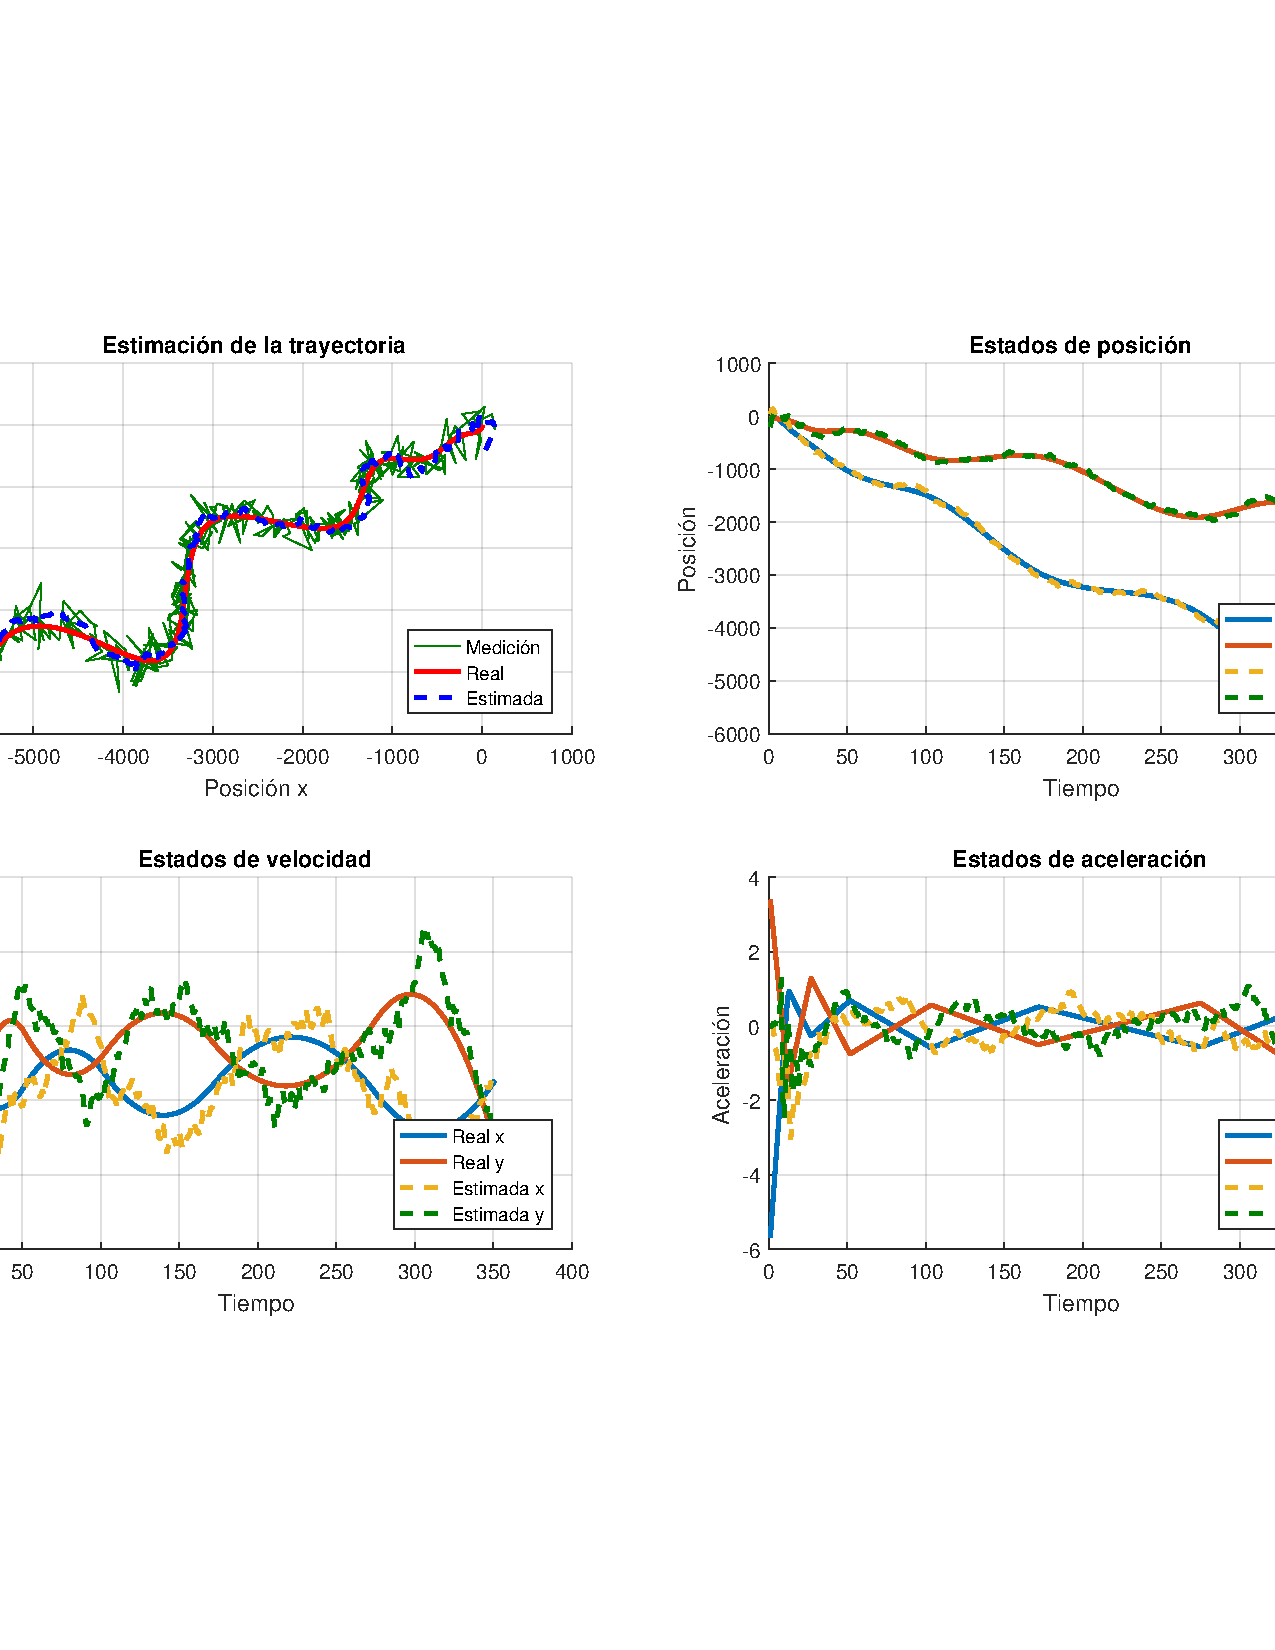
\includegraphics[width=1.0\textwidth,keepaspectratio]{Figuras/graf_ej2a.pdf}
			\caption{Caso: Medición De Posición}
			\label{fig:ej2a}
		\end{figure}
		
		En la figura \ref{fig:ej2a_innov} vemos la correlación de las innovaciones, puede verse de que se aproximan a un proceso blanco.
		
		\begin{figure}[H]
			\centering
			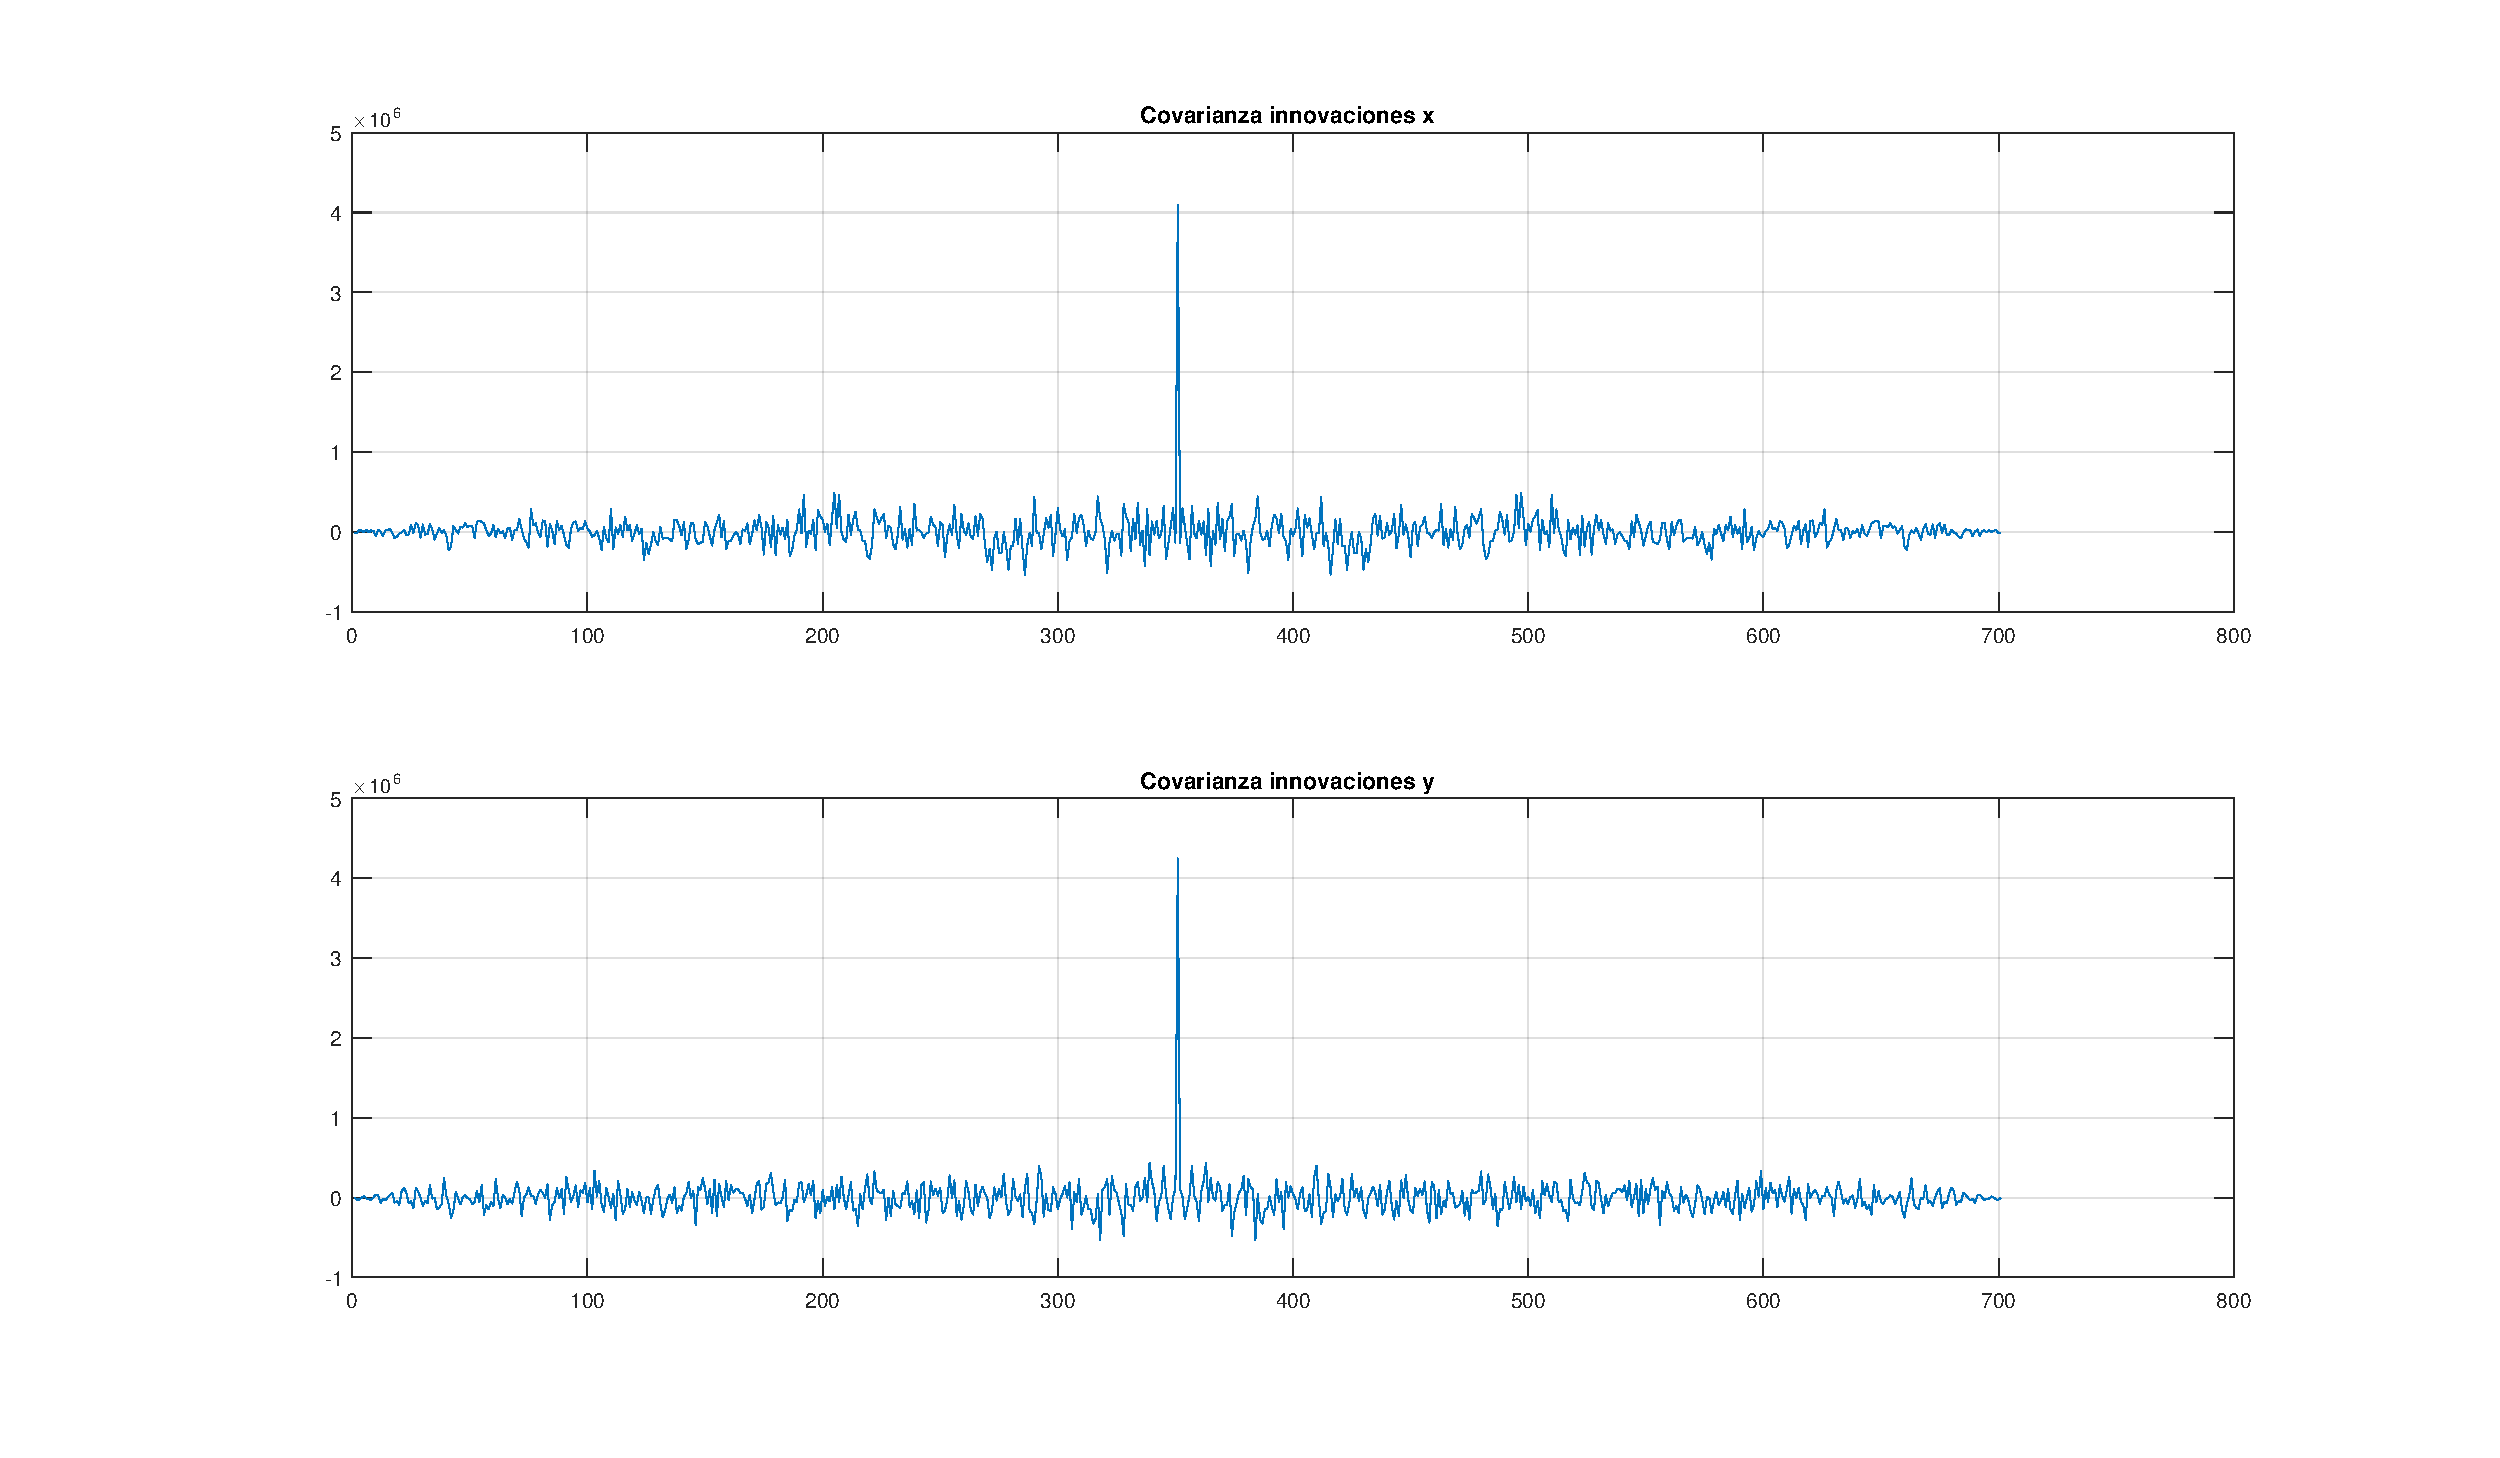
\includegraphics[width=1.0\textwidth,keepaspectratio]{Figuras/covinn_ej2a.pdf}
			\caption{Caso: Medición De Posición - Innovaciones}
			\label{fig:ej2a_innov}
		\end{figure}
		
		\subsubsection{Medición De Velocidad}
		
		En la figura \ref{fig:ej2b} observamos los resultados de la estimación basada en mediciones de velocidad. Puede verse que la estimación se desvía menos del valor real que las mediciones.
		
		\begin{figure}[H]
			\centering
			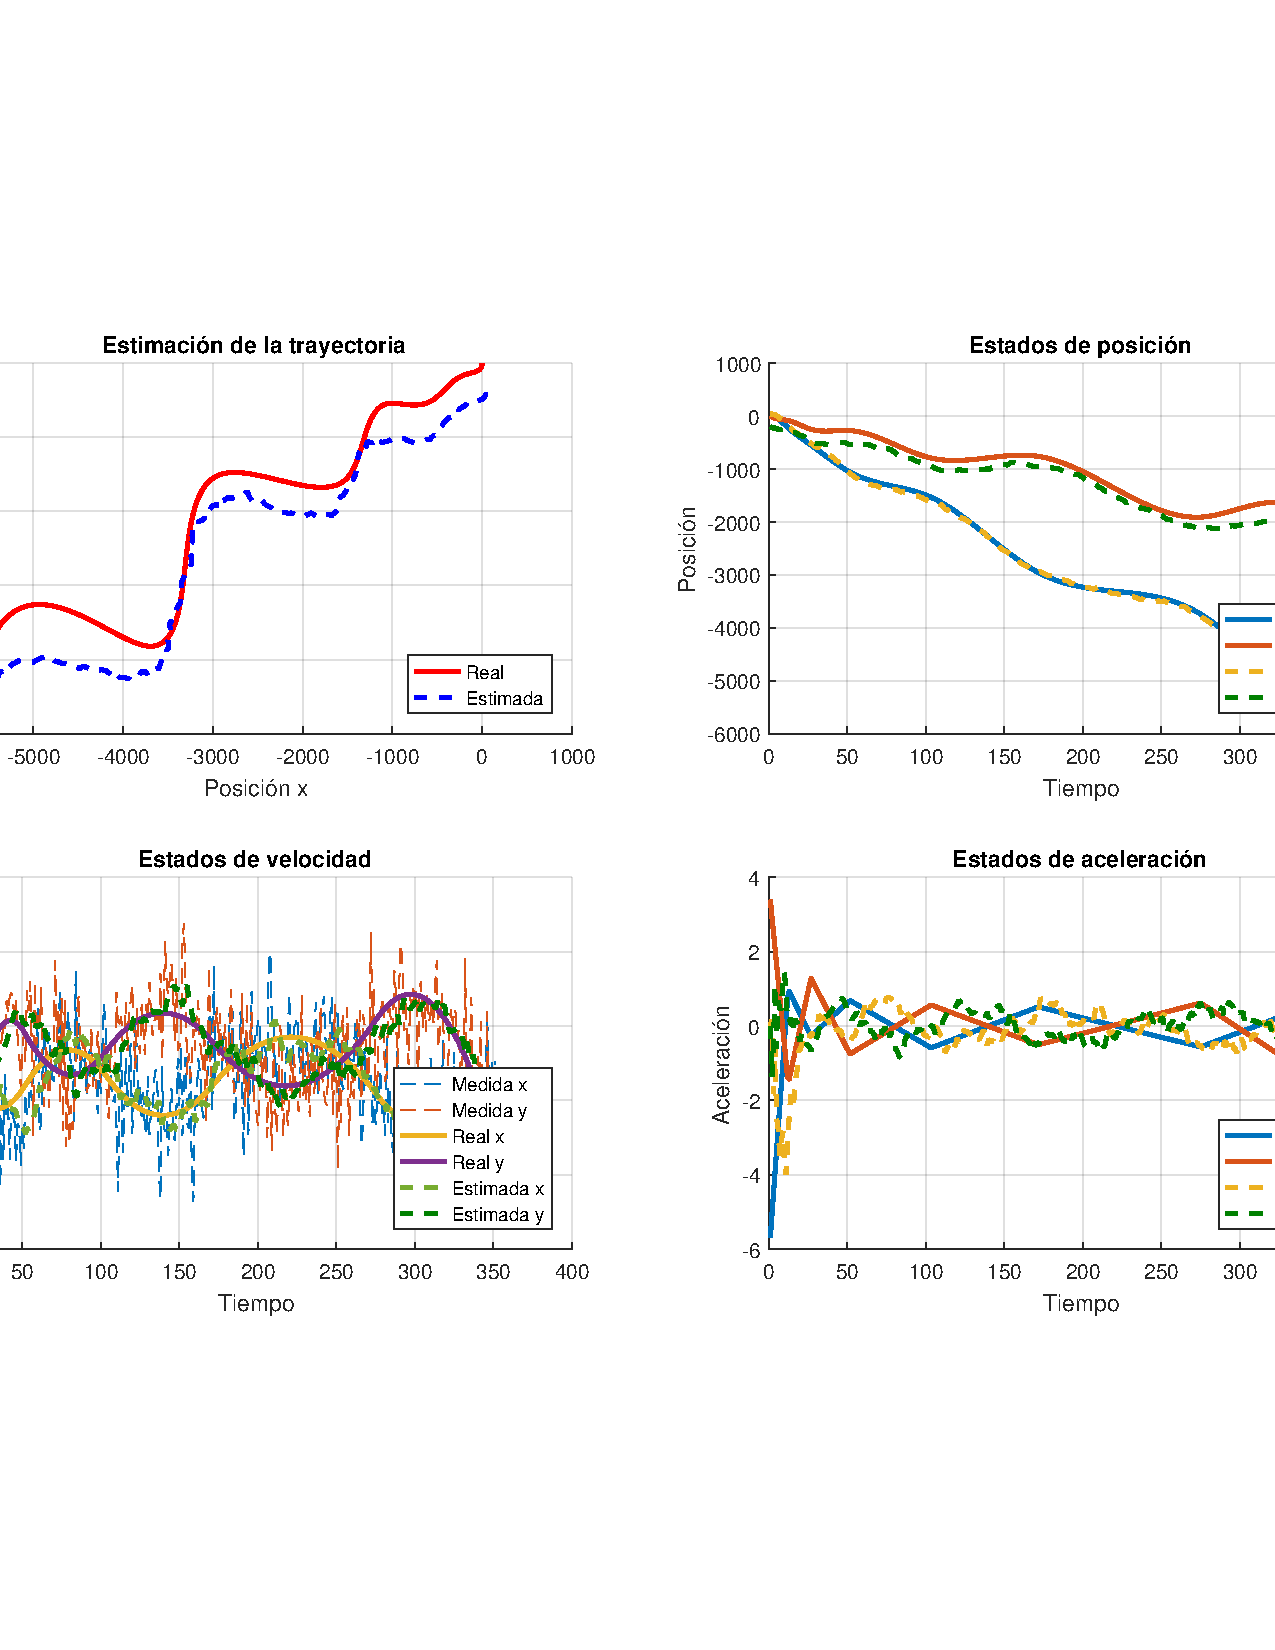
\includegraphics[width=1.0\textwidth,keepaspectratio]{Figuras/graf_ej2b.pdf}
			\caption{Caso: Medición De Velocidad}
			\label{fig:ej2b}
		\end{figure}
		
		En la figura \ref{fig:ej2b_innov} vemos la correlación de las innovaciones, puede verse de que se aproximan a un proceso blanco.
		
		\begin{figure}[H]
			\centering
			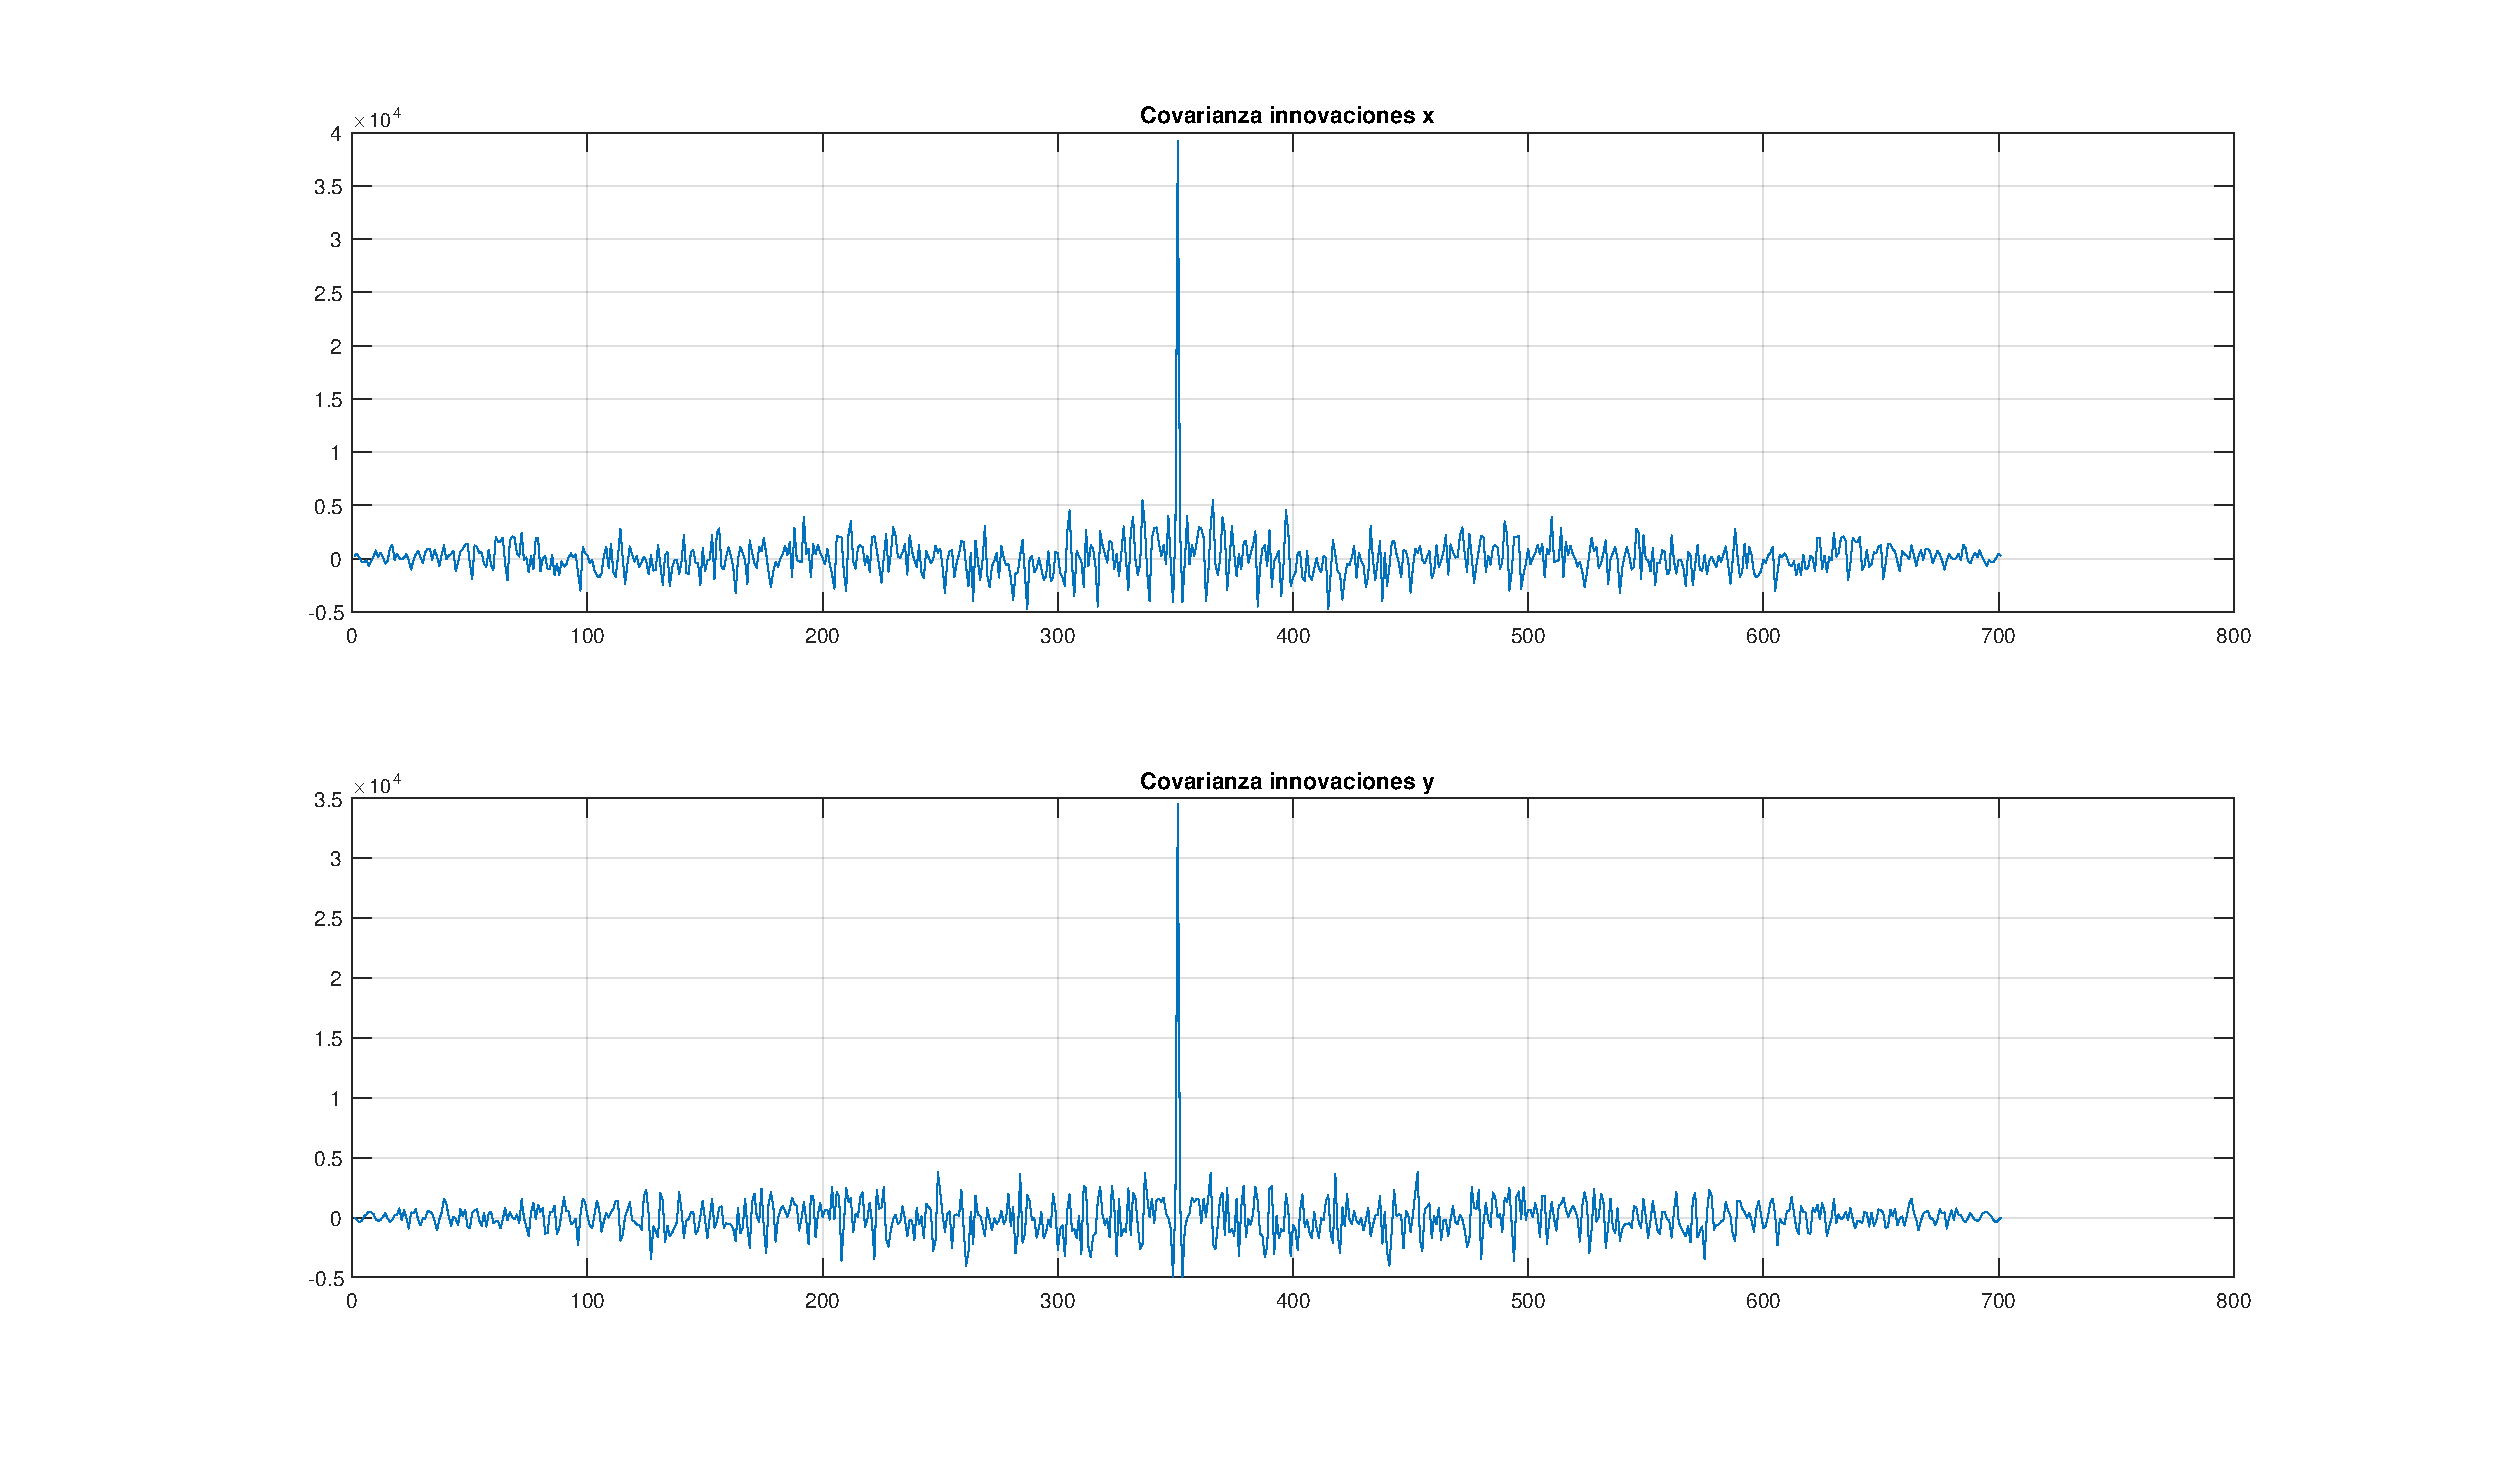
\includegraphics[width=1.0\textwidth,keepaspectratio]{Figuras/covinn_ej2b.pdf}
			\caption{Caso: Medición De Velocidad - Innovaciones}
			\label{fig:ej2b_innov}
		\end{figure}
			
		\subsubsection{Medición De Aceleración}
		
		En la figura \ref{fig:ej2c} observamos los resultados de la estimación basada en mediciones de aceleración. Puede verse que la estimación se desvía menos del valor real que las mediciones.
		
		\begin{figure}[H]
			\centering
			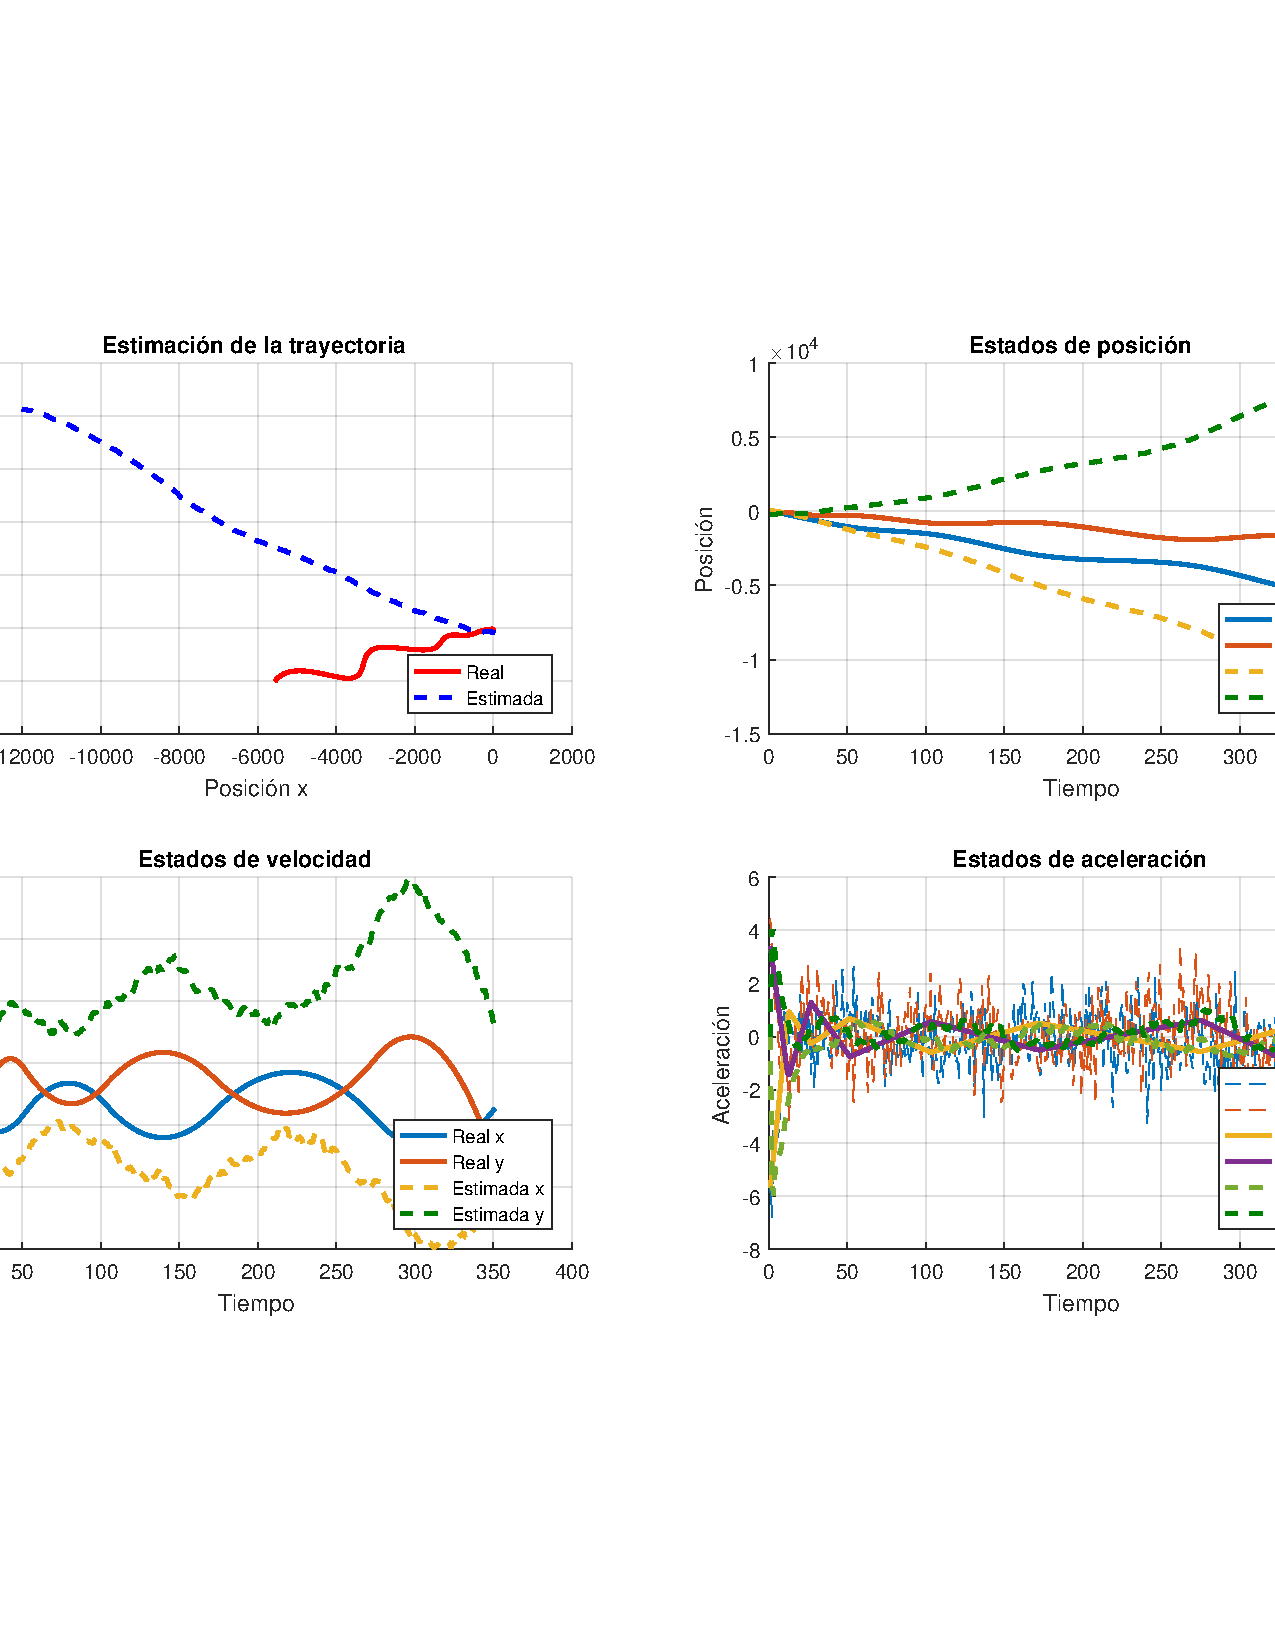
\includegraphics[width=1.0\textwidth,keepaspectratio]{Figuras/graf_ej2c.pdf}
			\caption{Caso: Medición De Aceleración}
			\label{fig:ej2c}
		\end{figure}
		
		En la figura \ref{fig:ej2c_innov} vemos la correlación de las innovaciones, puede verse de que se aproximan a un proceso blanco.
		
		\begin{figure}[H]
			\centering
			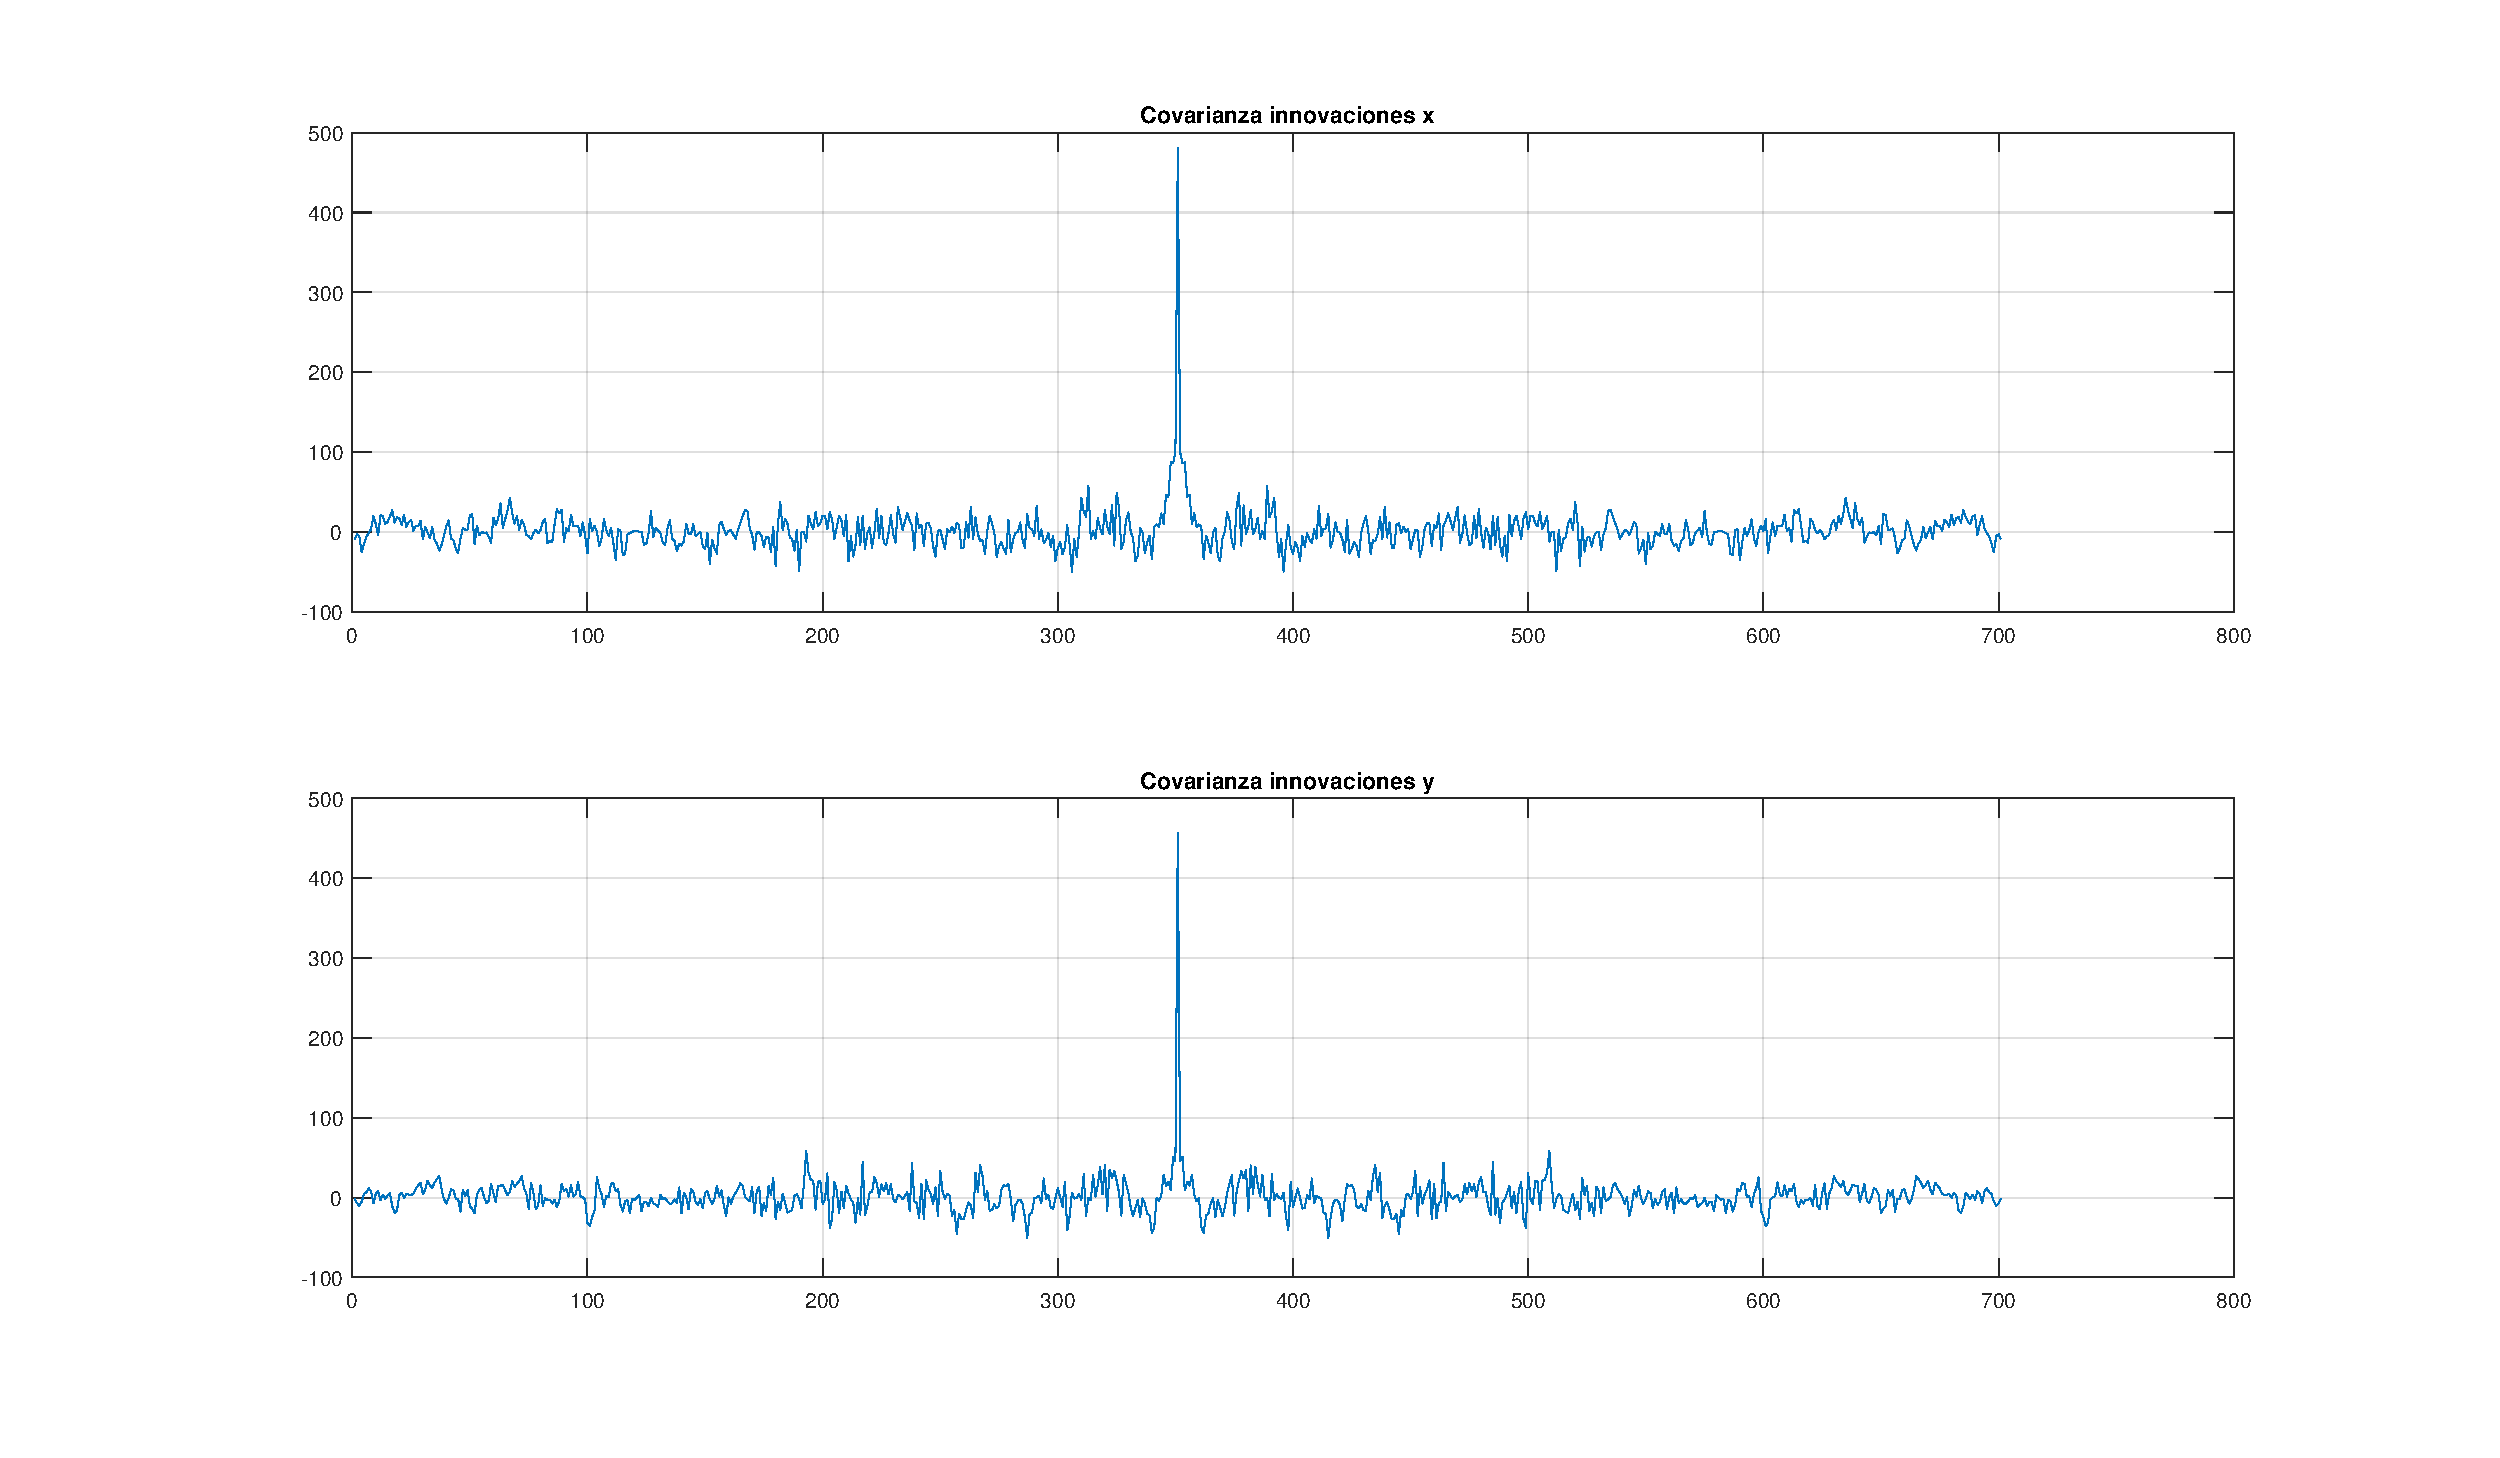
\includegraphics[width=1.0\textwidth,keepaspectratio]{Figuras/covinn_ej2c.pdf}
			\caption{Caso: Medición De Aceleración - Innovaciones}
			\label{fig:ej2c_innov}
		\end{figure}

%*% C = [eye(dim)*bool_p eye(dim)*bool_v eye(dim)*bool_a];	% Obsoleto
%*%C = [eye(dim)*bool_p eye(dim)*bool_v eye(dim)*bool_a];
%*%
%*%yk = C * ([Pos(:,1:dim) Vel(:,1:dim) Acel(:,1:dim)])' + randn(dim,cant_mediciones)*sigma_etap;

%*R = eye(dim)*sigma_etap^2;


	\section{Ejercicio 3 \\ Estimación Con Distintos Valores Inciales}\label{sec:ej3}
		
	\begin{lstlisting}[caption = Parte del \emph{Script} utilizado para el ejercicio 3]
% Nuevos datos
x01 = [40 -200 0 0 0 0]';
x02 = [200 -3000 0 0 0 0]';
x03 = x01;
x04 = x02;
x0_vec = [x01 x02 x03 x04];

diag1_p = [100^4 100^4, 10^2 10^2, 10 10];
diag2_p = [0.1 0.1, 1e-5 1e-5, 1e-7 1e-7];
diag_vec = [diag1_p; diag1_p; diag2_p; diag2_p];


for l = 1:4
	xa = x0_vec(:,l);
	Pa = diag(diag_vec(l,:));
	xk1_k1 = xa;
	Pk1_k1 = Pa;

	for i = 1:cant_mediciones-1
		% Predicción
		xk_k1 = Ad * xk1_k1;
		Pk_k1 =	Ad * Pk1_k1 * Ad' + Bk1 * Qd * Bk1.';
	
		% Corrección
		Kk = Pk_k1 * C'*(R + C*Pk_k1*C')^-1;
		xk_k = xk_k1 + Kk*(yk(i,:)' - C*xk_k1);
		Pk_k = (eye(dim*3) - Kk*C) * Pk_k1;
		
		% Actualización
		xk1_k1 = xk_k;
		Pk1_k1 = Pk_k;
	
	
		% Guardo
		xa = [xa xk_k];
		Pa = [Pa; Pk_k];
	end

	if(l==1)
		x1=xa; P1=Pa;
	elseif(l==2)
		x2=xa; P2=Pa;
	elseif(l==3)
		x3=xa; P3=Pa;
	else
		x4=xa; P4=Pa;
	end
	
end
	\end{lstlisting}

	\graficarEPS{1}{graf_ej3_superpuesto}{Superposición de las trayectorias estimadas con distintos valores iniciales.}{fig:ej3_sup}
	\graficarEPS{1}{graf_ej3a}{Estimación de la trayectoria a partir de $x_1$ y $P_1$.}{fig:ej3a}
	\graficarEPS{1}{graf_ej3b}{Estimación de la trayectoria a partir de $x_2$ y $P_2$.}{fig:ej3b}
	\graficarEPS{1}{graf_ej3c}{Estimación de la trayectoria a partir de $x_3$ y $P_3$.}{fig:ej3c}
	\graficarEPS{1}{graf_ej3d}{Estimación de la trayectoria a partir de $x_4$ y $P_4$.}{fig:ej3d}


	\section{Ejercicio 4 \\ Estimación Con Sesgo}\label{sec:ej4}
		\subsection{Fundamentos}

	Cuando se trabaja con sensores con ruido de media desconocida, no nula y constante, se propone el siguiente modelo:

	\begin{equation*}
		\vect{\eta}_{n} = \vect{\tilde{\eta}}_{n} + \vect{\mu}
	\end{equation*}

	\begin{equation*}
		\Sigma_{d}:
		\begin{cases}
			\vect{x}_{n + 1} = A_{d}\: \vect{x}_{n} + B_{d} \: \vect{\xi}_{n} \\
			\vect{y}_{n} = C_{d}\: \vect{x}_{n} + \vect{\tilde{\eta}}_{n} + \vect{\mu}
		\end{cases}
	\end{equation*}
	donde ahora el nuevo ruido $\vect{\tilde{\eta}}_{n}$ es de media nula, y se representa la media del ruido como $\vect{\mu}$. Una técnica para llevar el nuevo modelo a la forma del modelo anterior consiste en considerar la media del ruido como un estado más a estimar. De esta forma se incluye dentro de las variables de estado:

	\begin{equation*}
		\vect{z}_{n} = \begin{bmatrix} \vect{x}_{n} \\[0.3em] \vect{\mu}\end{bmatrix} \qquad%
	\end{equation*}
	resultando en:
	
	\begin{equation*}
		\tilde{\Sigma_{d}}:
		\begin{cases}
			\vect{z}_{n + 1} = \tilde{A_{d}}\: \vect{z}_{n} + \tilde{B_{d}} \: \vect{\xi}_{n} \\
			\vect{y}_{n} = \tilde{C_{d}}\: \vect{z}_{n} + \vect{\tilde{\eta}}_{n}
		\end{cases}
	\end{equation*}

	Con las nuevas matrices:
	
	\begin{equation*}
			\tilde{A_{d}} = \begin{bmatrix} A_{d} & 0 \\[0.3em] 0 & I \end{bmatrix}
	\end{equation*}
	
	\begin{equation*}
			\tilde{B_{d}} = \begin{bmatrix} B_{d} \\[0.3em] 0 \end{bmatrix}
	\end{equation*}
	
	\begin{equation*}
			\tilde{C_{d}} = \begin{bmatrix} C_{d} & I \end{bmatrix}
	\end{equation*}
	
	Cabe aclarar que el éxito de esta solución dependerá de la observabilidad del nuevo sistema. A continuación se expondrán las distintas variantes que pueden darse en cuanto a la observabilidad.

%--------------------------------------------------------------------------------------------------

\subsection{Medición de P - Sesgo en P}

	En la Figura \ref{fig:ej4a} se observa el resultado de medir sólo posición, con un sesgo en la misma. En el gráfico, sin la estimación del sesgo, la estimación de la trayectoria se encuentra desviada de la real, de la misma manera que lo están las mediciones. Sin embargo, como en este caso el sesgo no es observable, el resultado estimando con o sin sesgo es el mismo.

	\begin{figure}[H]
		\centering
		%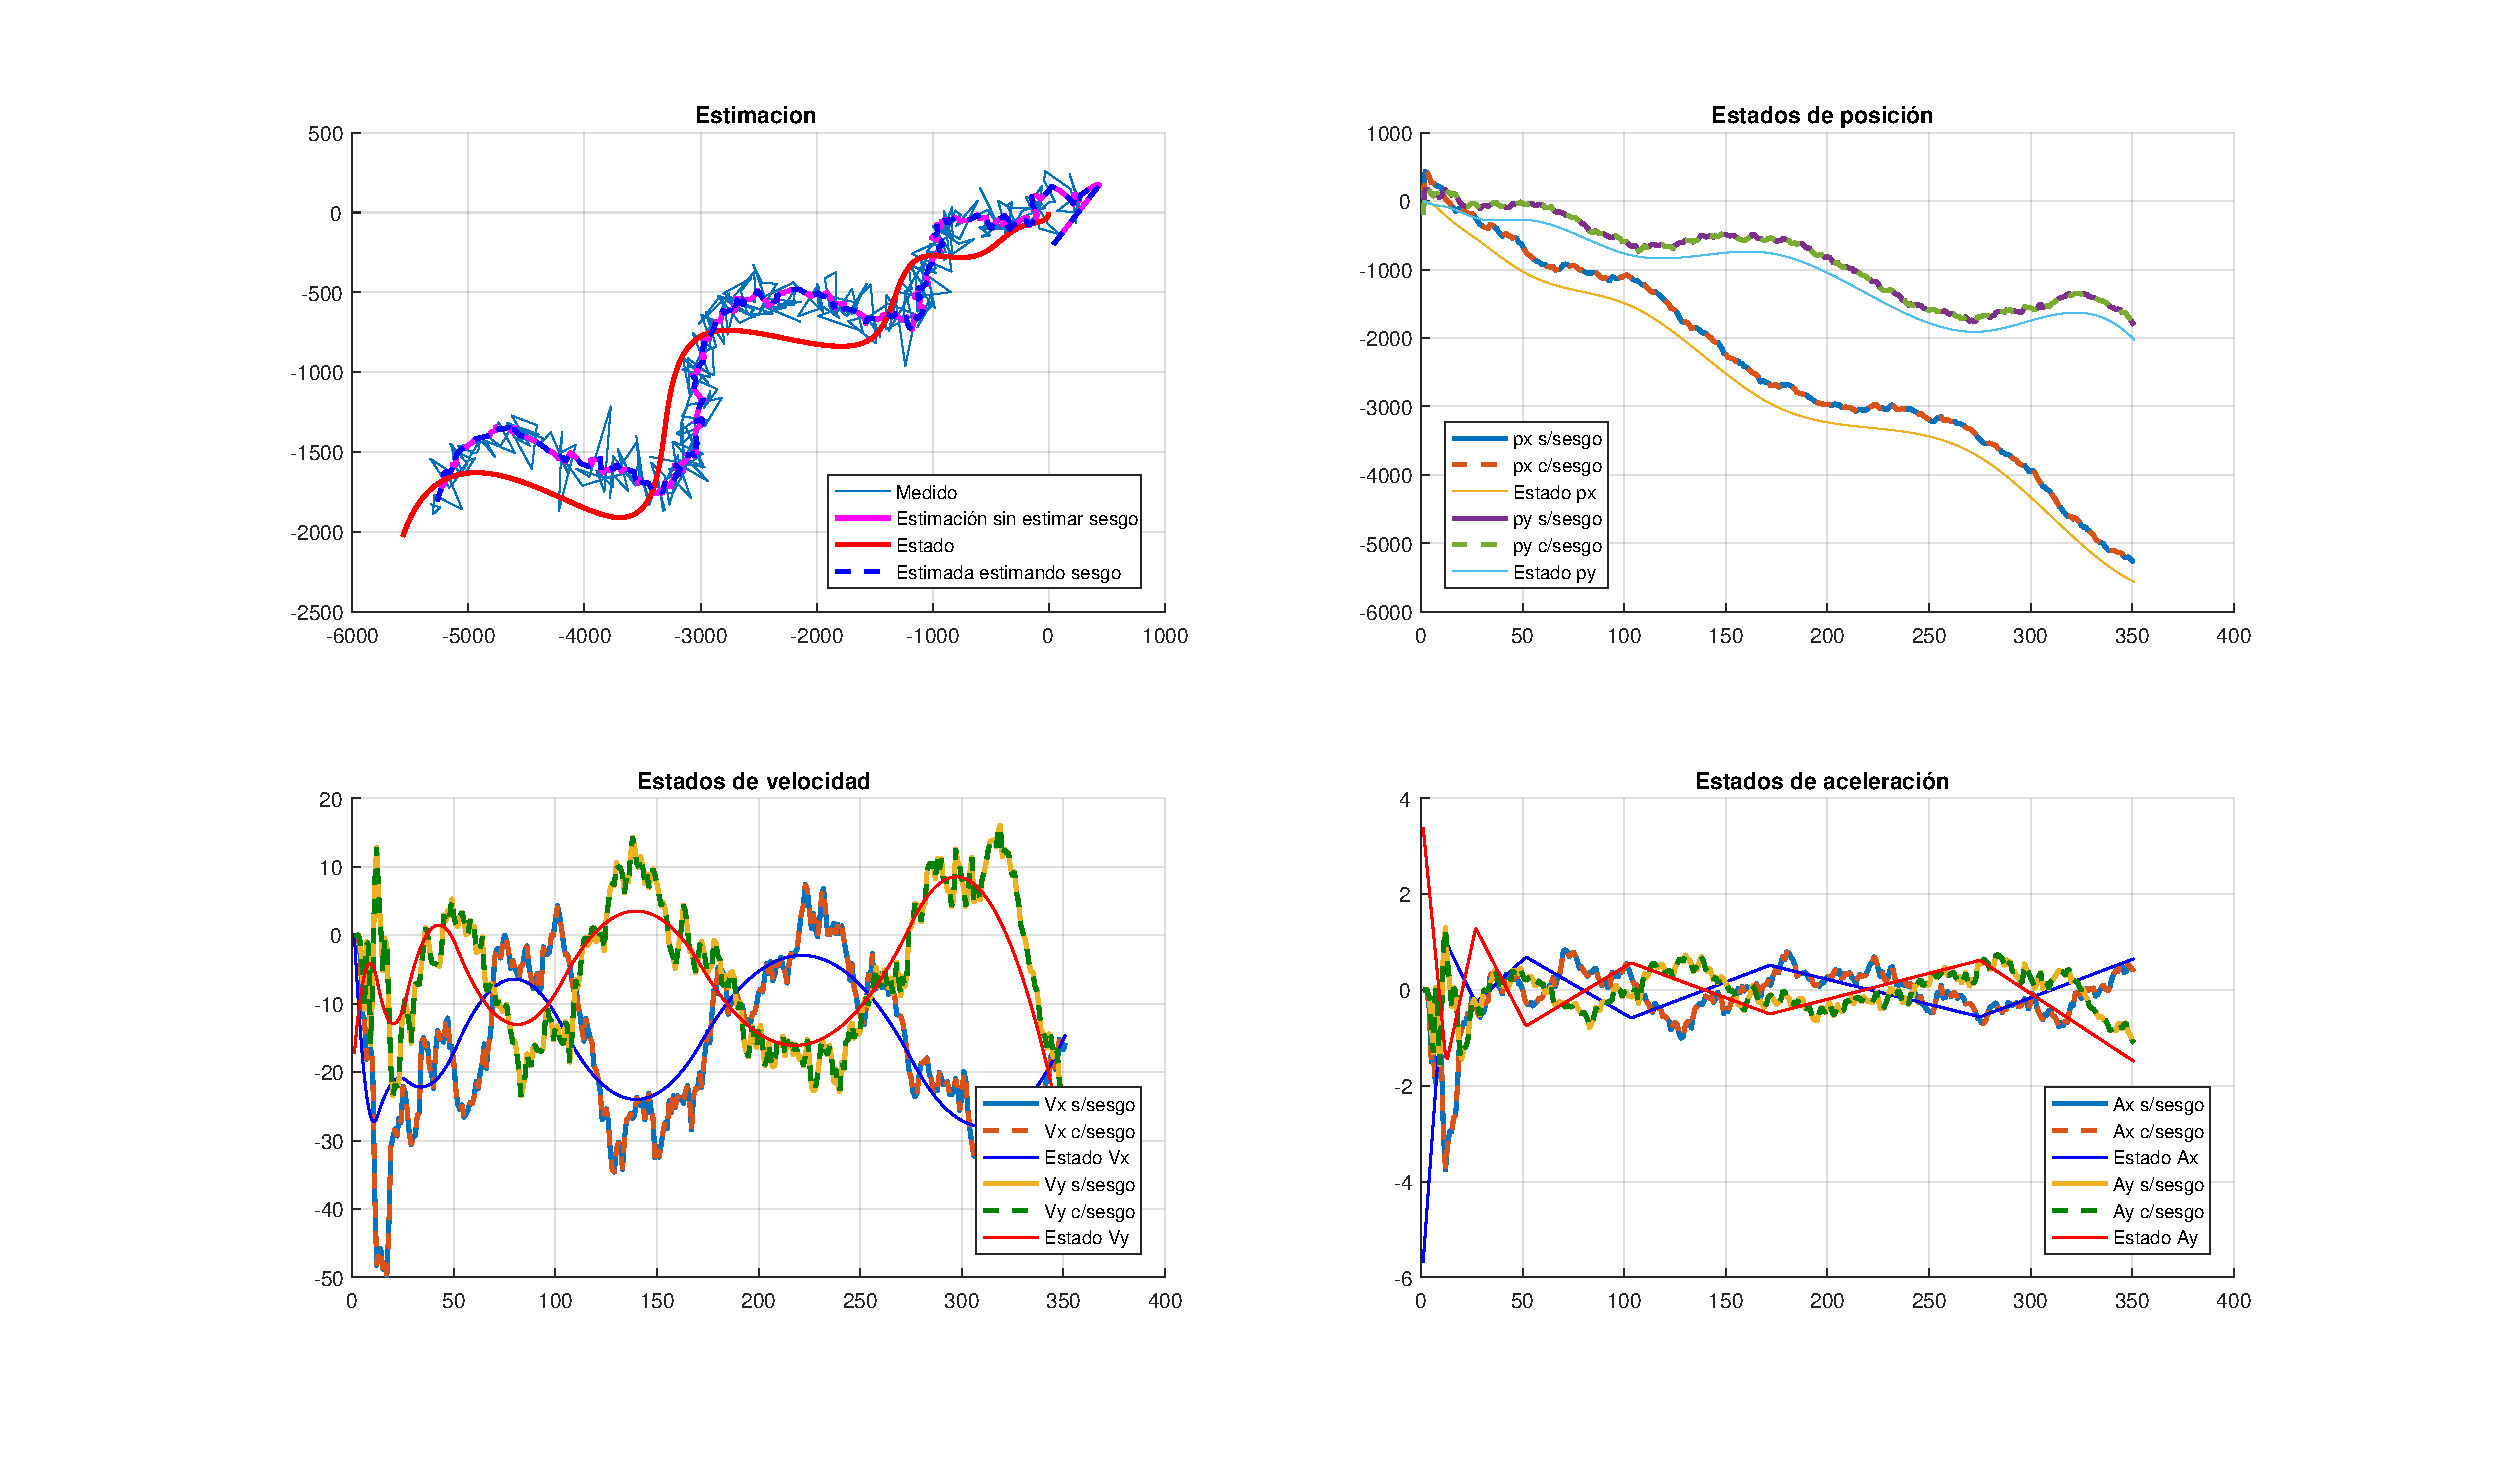
\includegraphics[width=1.0\textwidth,keepaspectratio]{Figuras/graf_ej4a.pdf}
		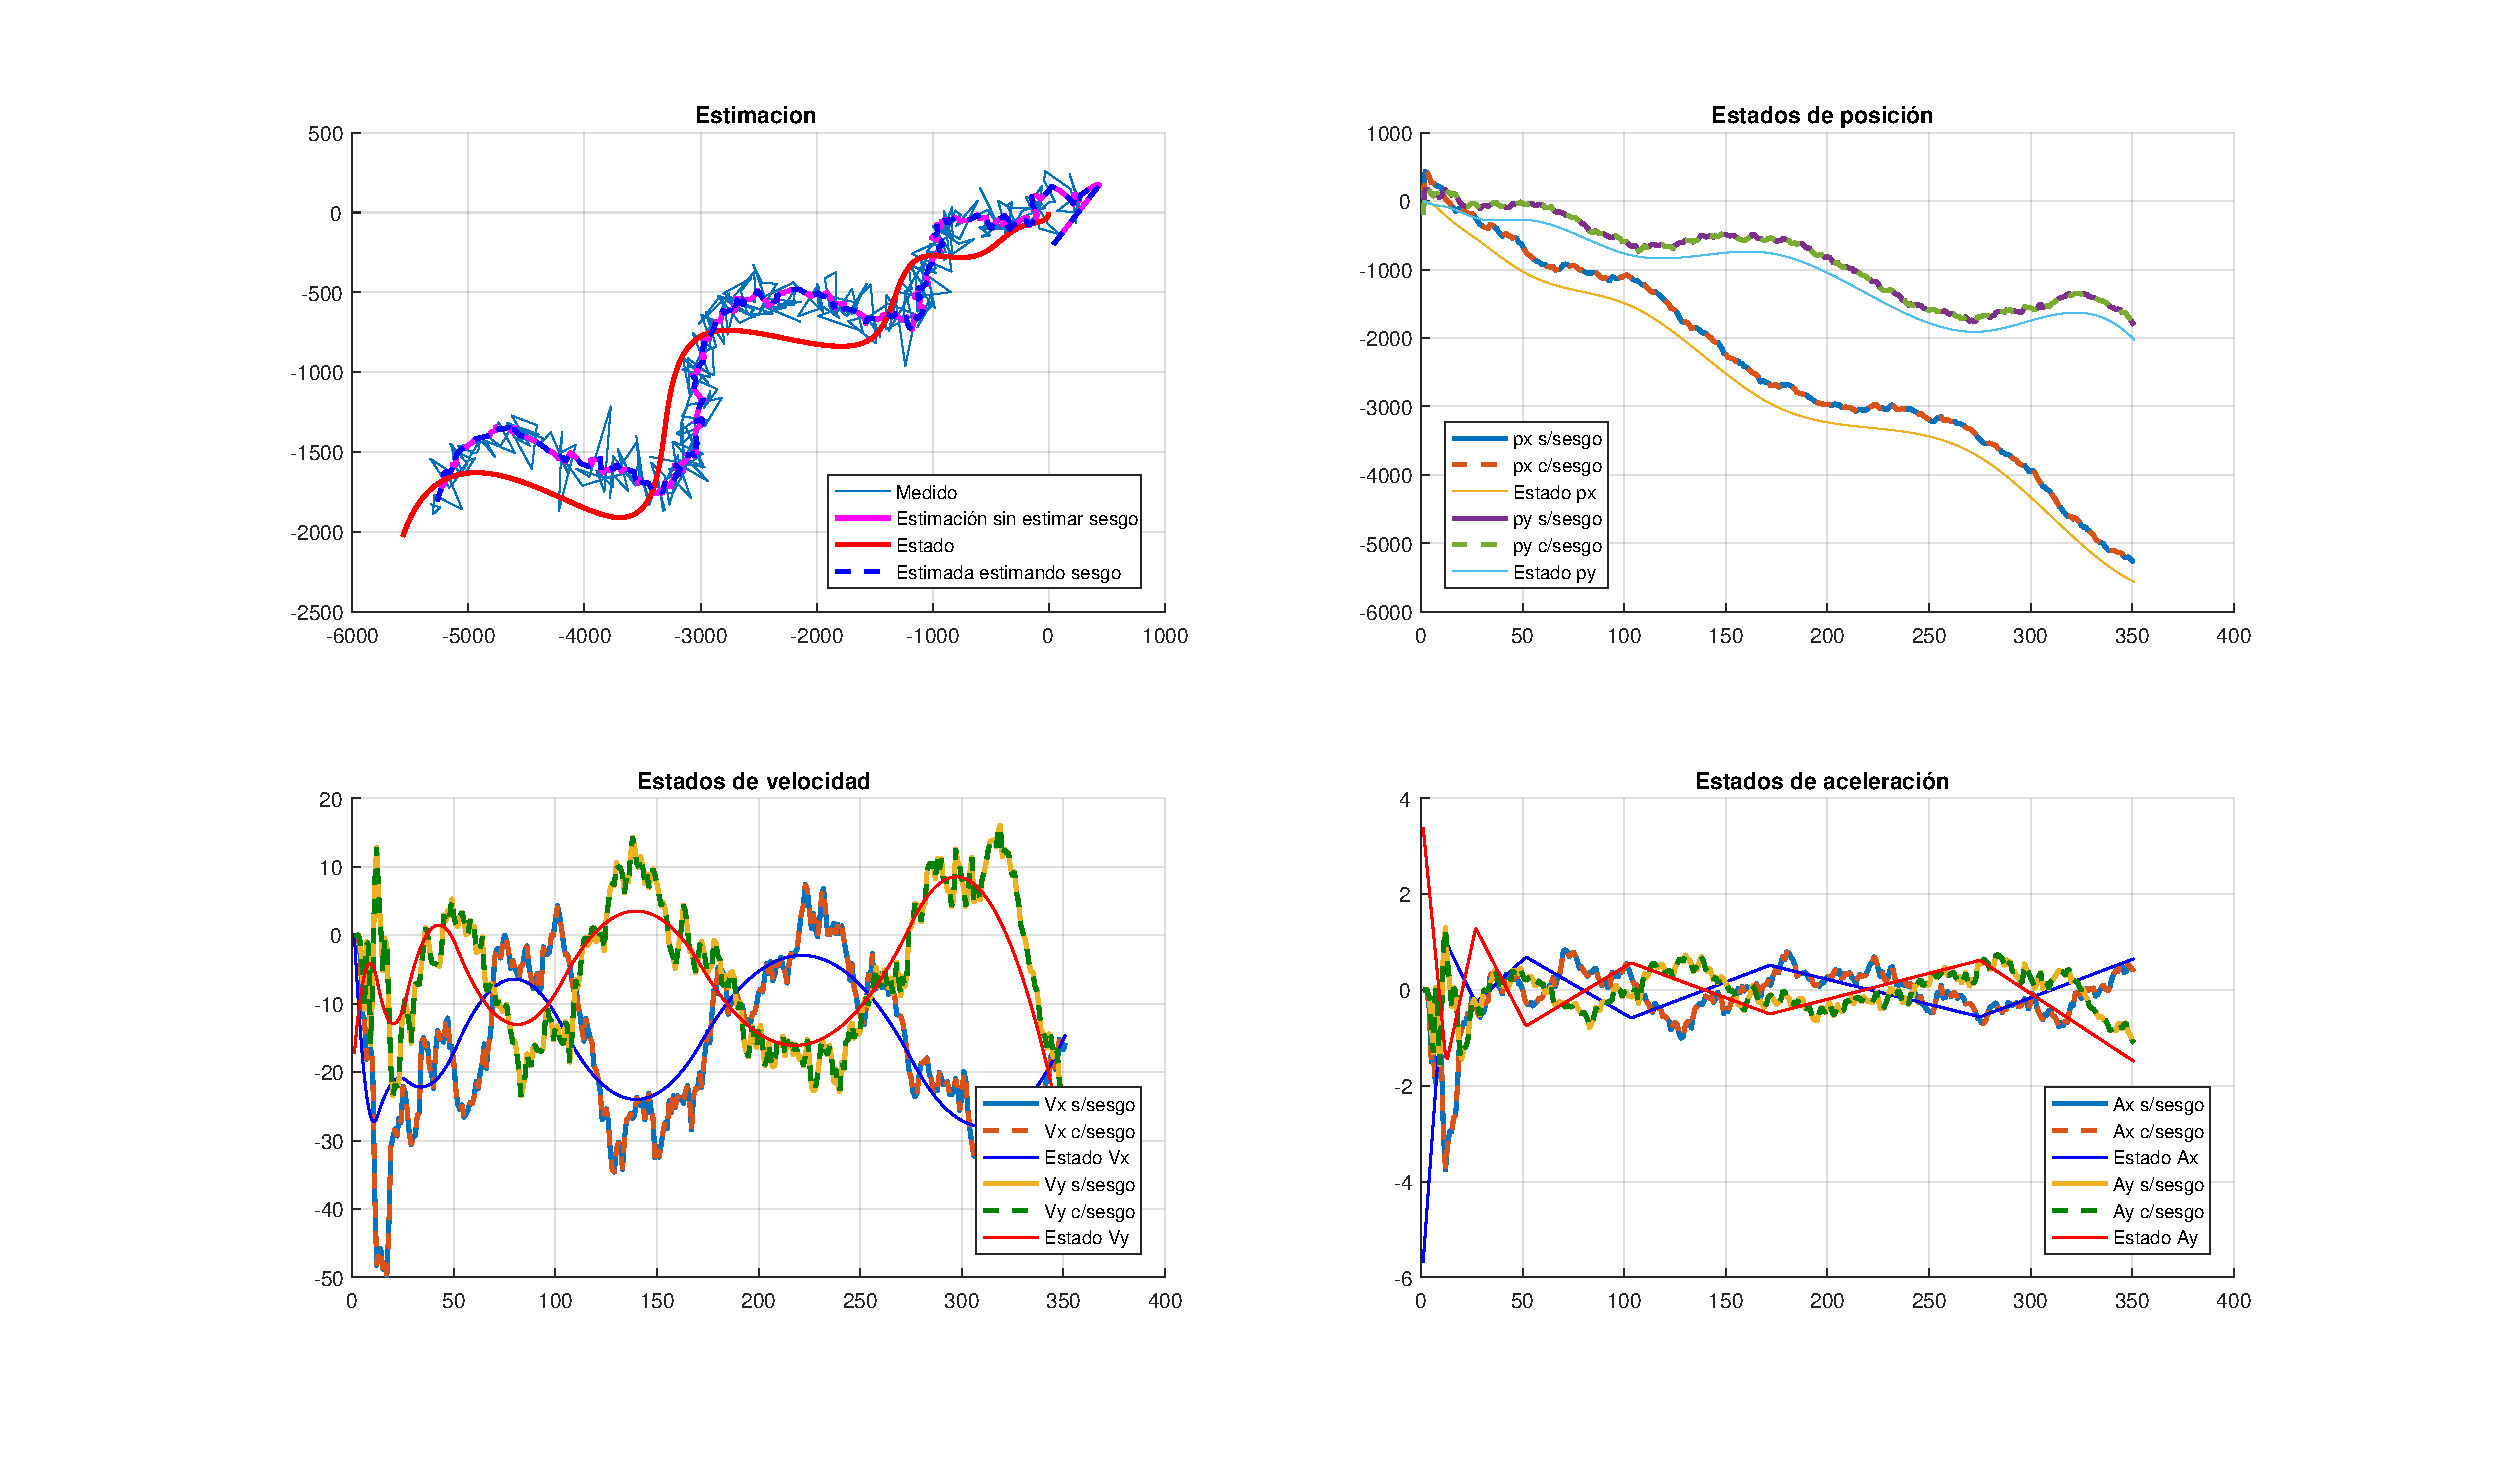
\includegraphics[scale=0.5,trim={6,5cm 0 0 0}]{Figuras/graf_ej4a.pdf}
		\caption{Estimación De Trayectoria}
		\label{fig:ej4a}
	\end{figure}
	
	En la Figura \ref{fig:ej4a_bias} se observa la convergencia de la estimación del sesgo. Es posible ver que no converge exactamente al valor deseado ($\vect{b}_p = [\SI{300}{\m}\; \SI{200}{\m}]^T$).
	
	\begin{figure}[H]
		\centering
		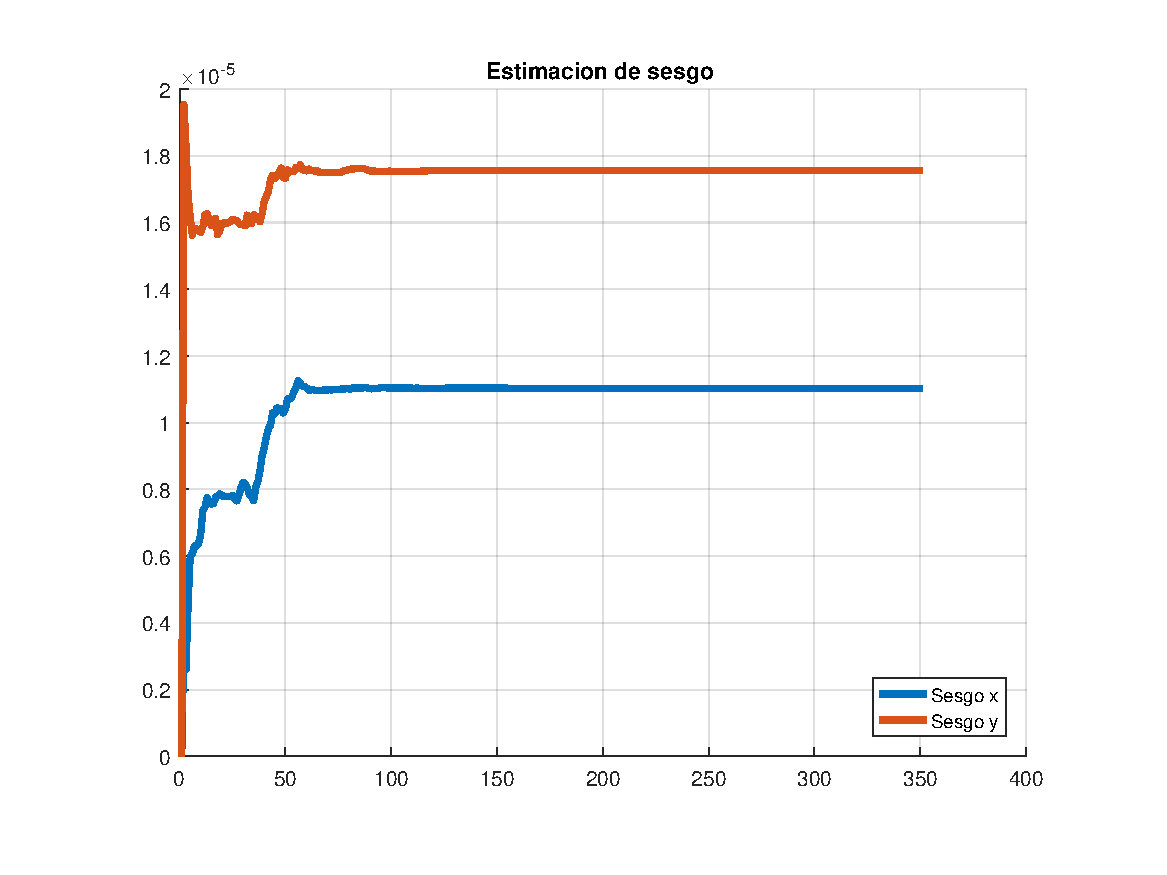
\includegraphics[width=0.7\textwidth,keepaspectratio]{Figuras/bias_ej4a.pdf}
		\caption{Estimación Del Sesgo}
		\label{fig:ej4a_bias}
	\end{figure}
	
	En la Figura \ref{fig:ej4a_cov} se observa la autocorrelación de las innovaciónes. Es posible ver que se trata de un proceso blanco.
	
	\begin{figure}[H]
		\centering
		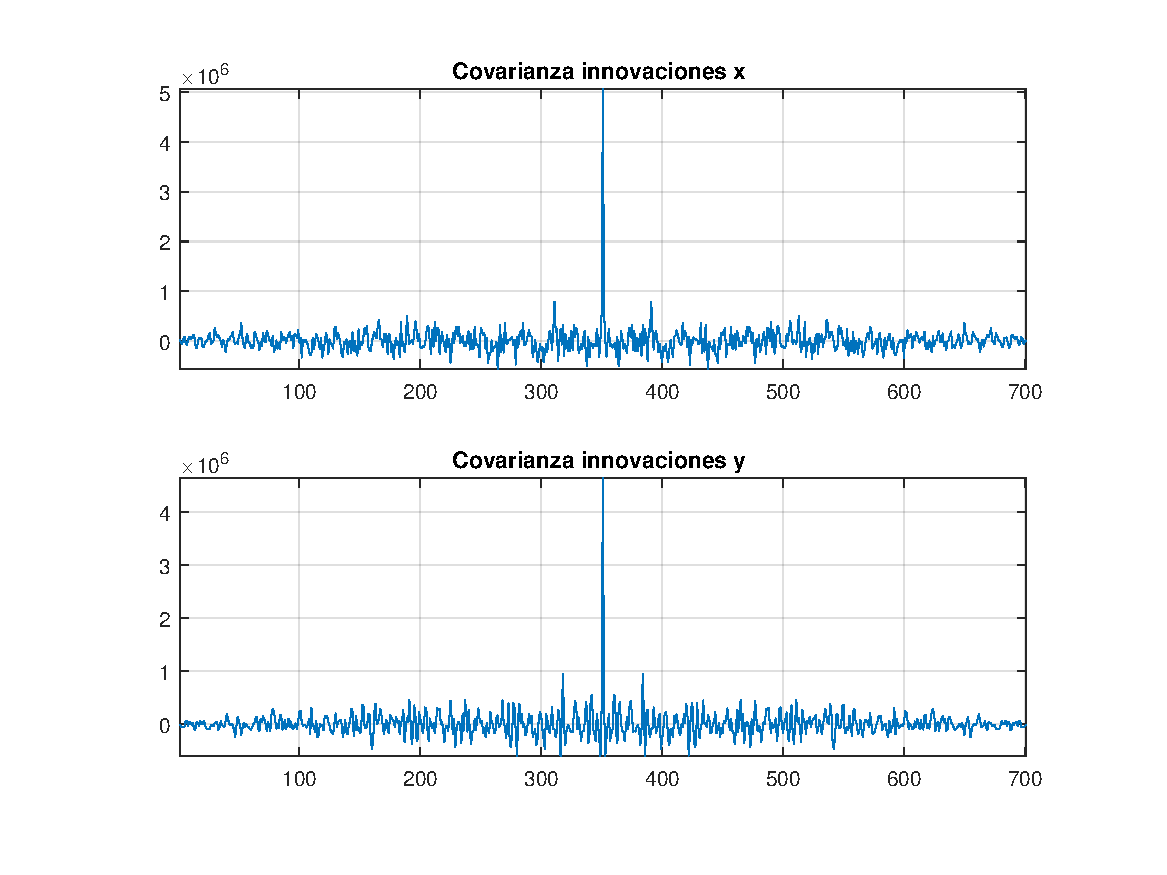
\includegraphics[width=1.0\textwidth,keepaspectratio]{Figuras/covinn_ej4a.pdf}
		\caption{Correlación De Innovaciones}
		\label{fig:ej4a_cov}
	\end{figure}
	
%--------------------------------------------------------------------------------------------------

\subsection{Medición de PVA - Sesgo en P}

	En la Figura \ref{fig:ej4b} se observa el resultado de la estimación de la trayectoria. Éste resulta similar al caso anterior, dado que tampoco se tiene observabilidad en el sesgo.

	\begin{figure}[H]
		\centering
		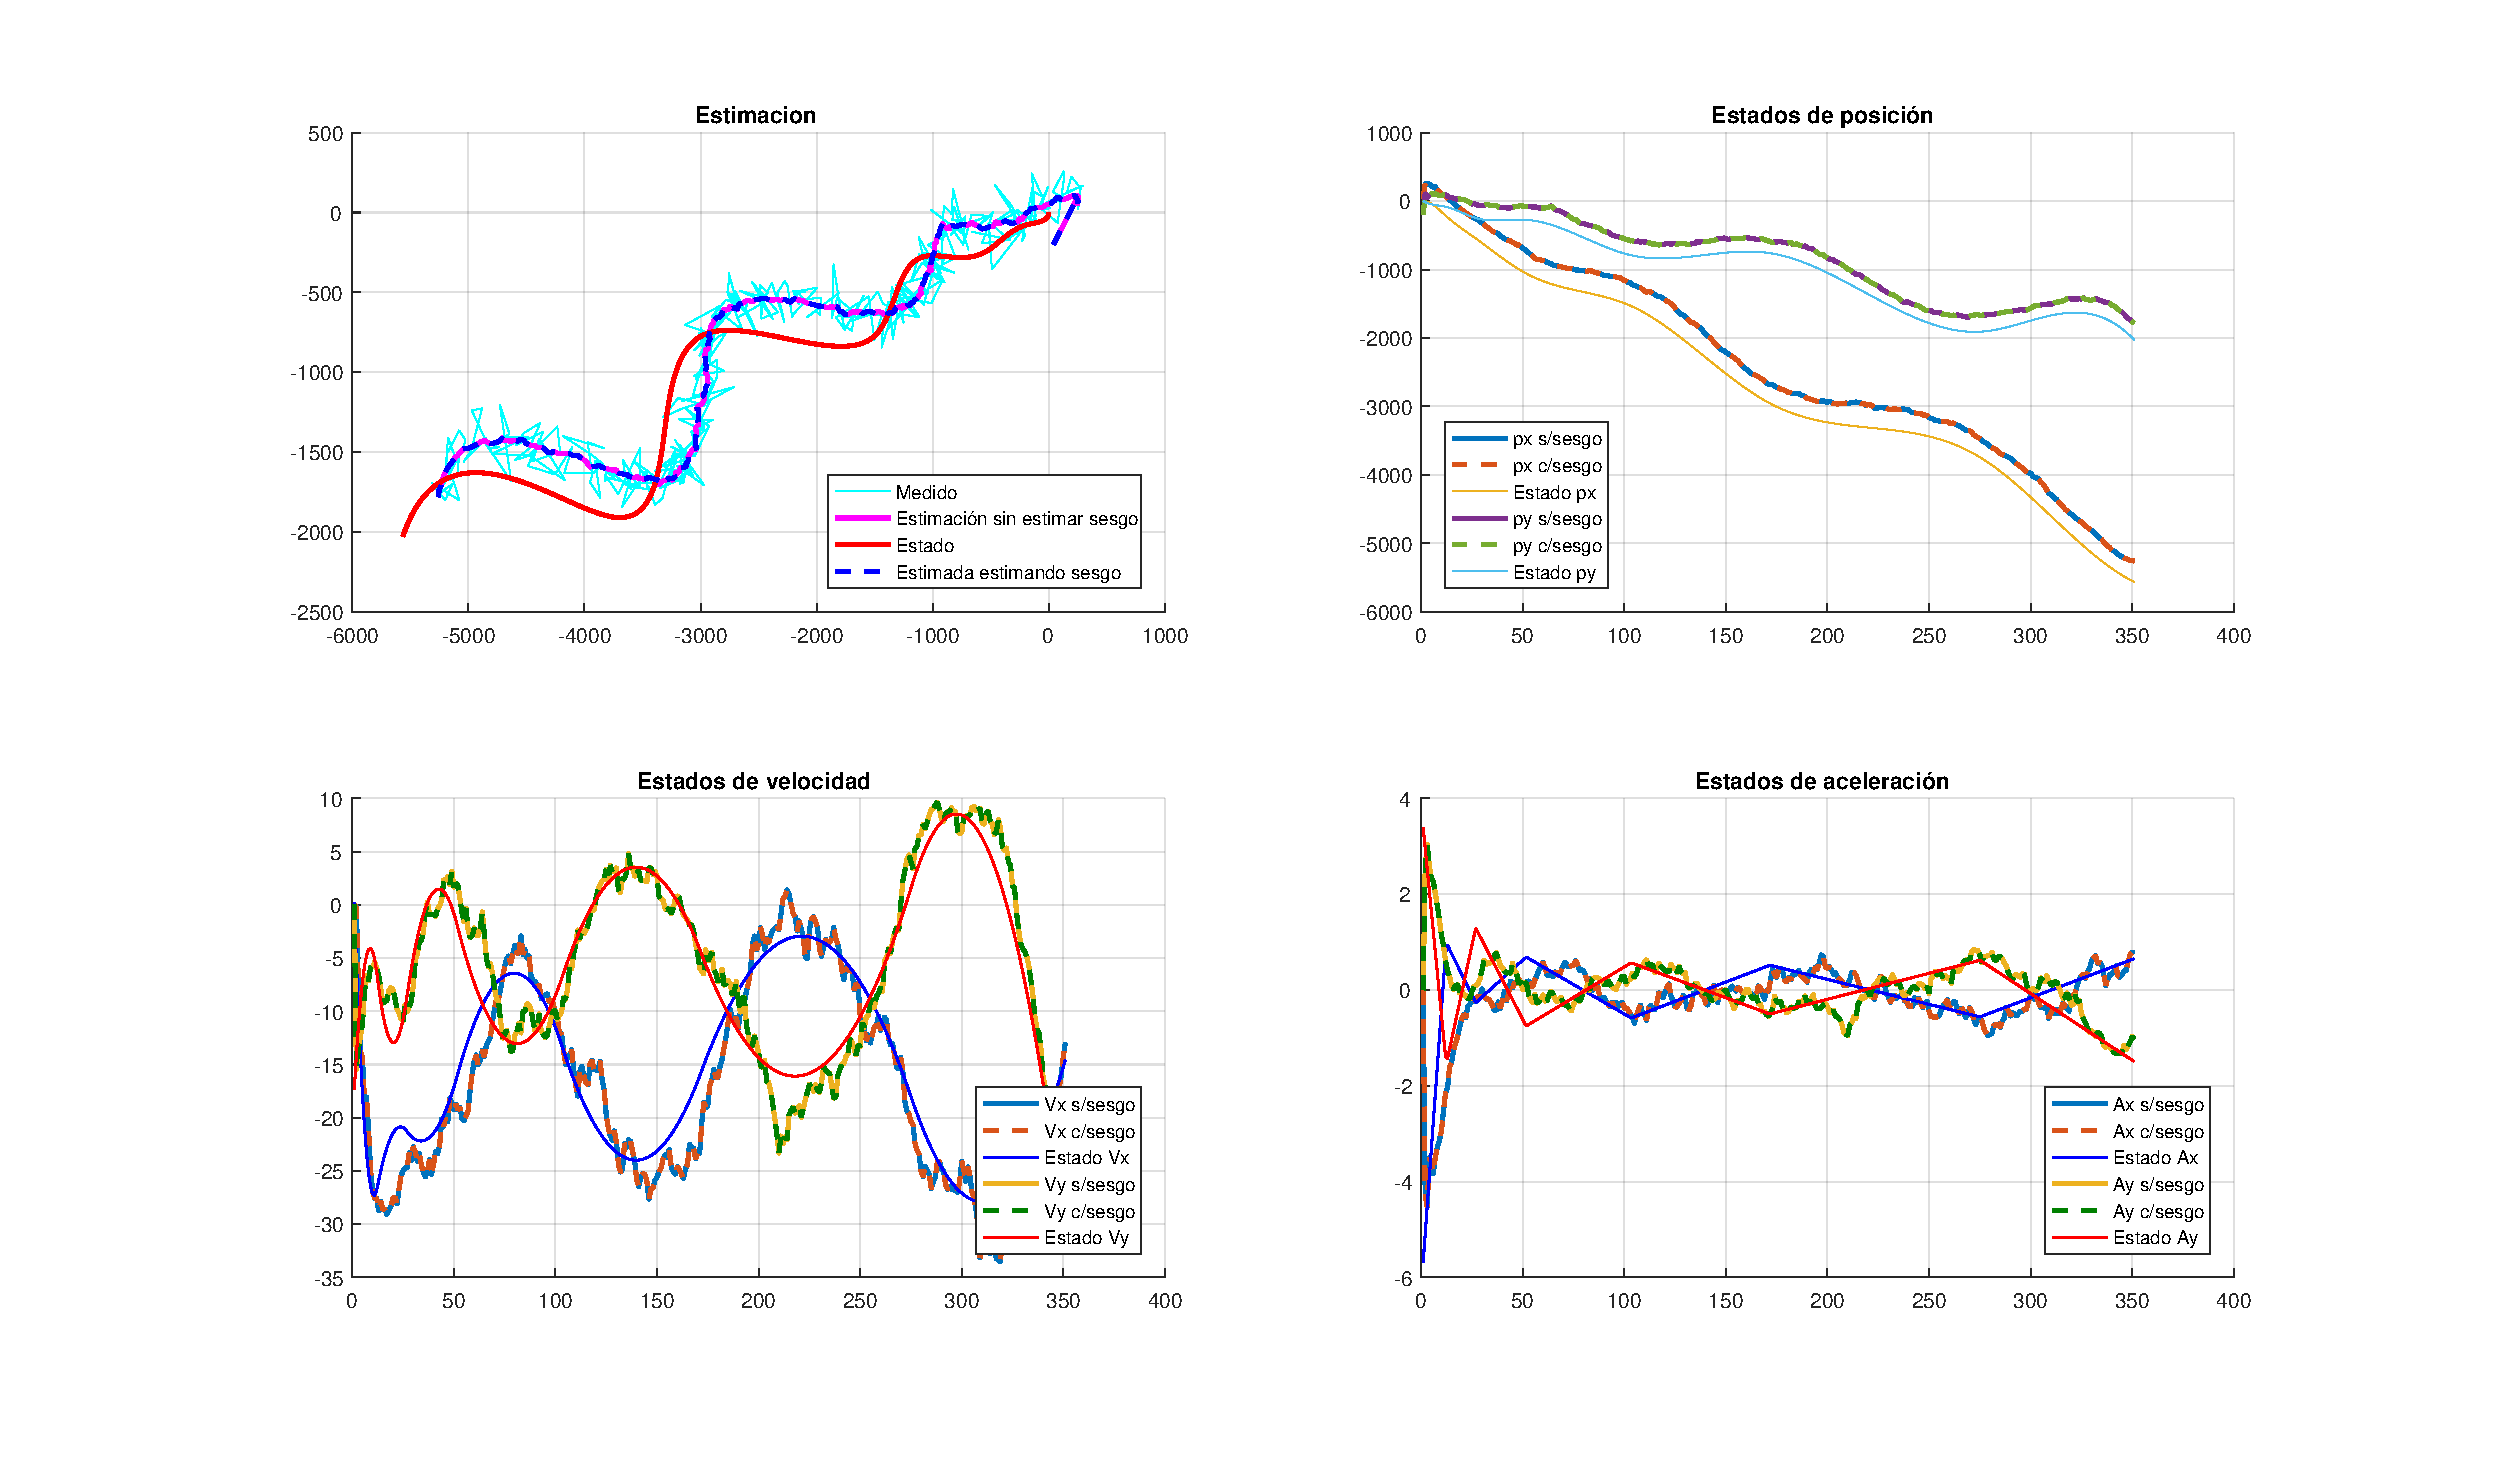
\includegraphics[scale=0.5,trim={6,5cm 0 0 0}]{Figuras/graf_ej4b.pdf}
		\caption{Estimación De Trayectoria}
		\label{fig:ej4b}
	\end{figure}
	
	En la Figura \ref{fig:ej4b_bias} se observa la convergencia de la estimación del sesgo. Es posible ver que no converge exactamente al valor deseado, al igual que en el caso anterior.
	
	\begin{figure}[H]
		\centering
		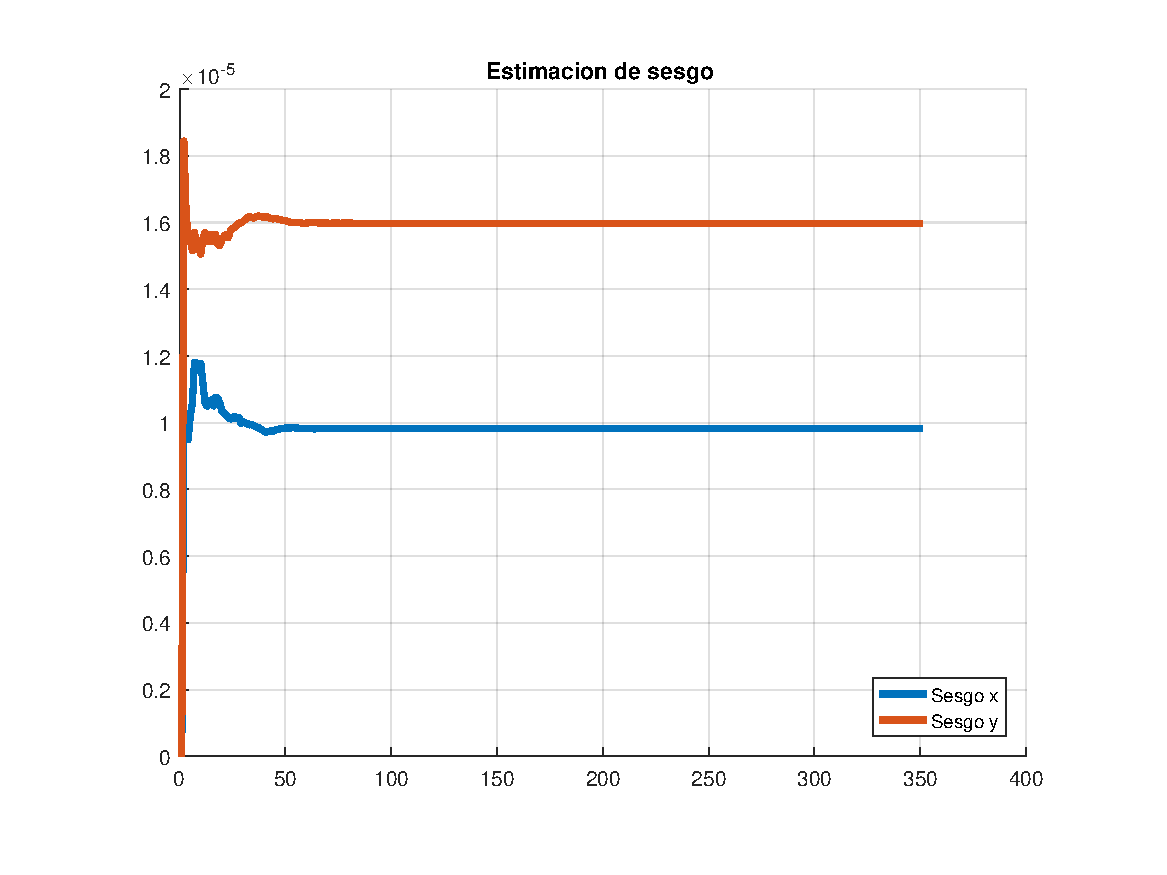
\includegraphics[width=0.7\textwidth,keepaspectratio]{Figuras/bias_ej4b.pdf}
		\caption{Estimación Del Sesgo}
		\label{fig:ej4b_bias}
	\end{figure}
	
	En la Figura \ref{fig:ej4b_cov} se observa la autocorrelación de las innovaciónes. Es posible ver que se trata de un proceso blanco.
	
	\begin{figure}[H]
		\centering
		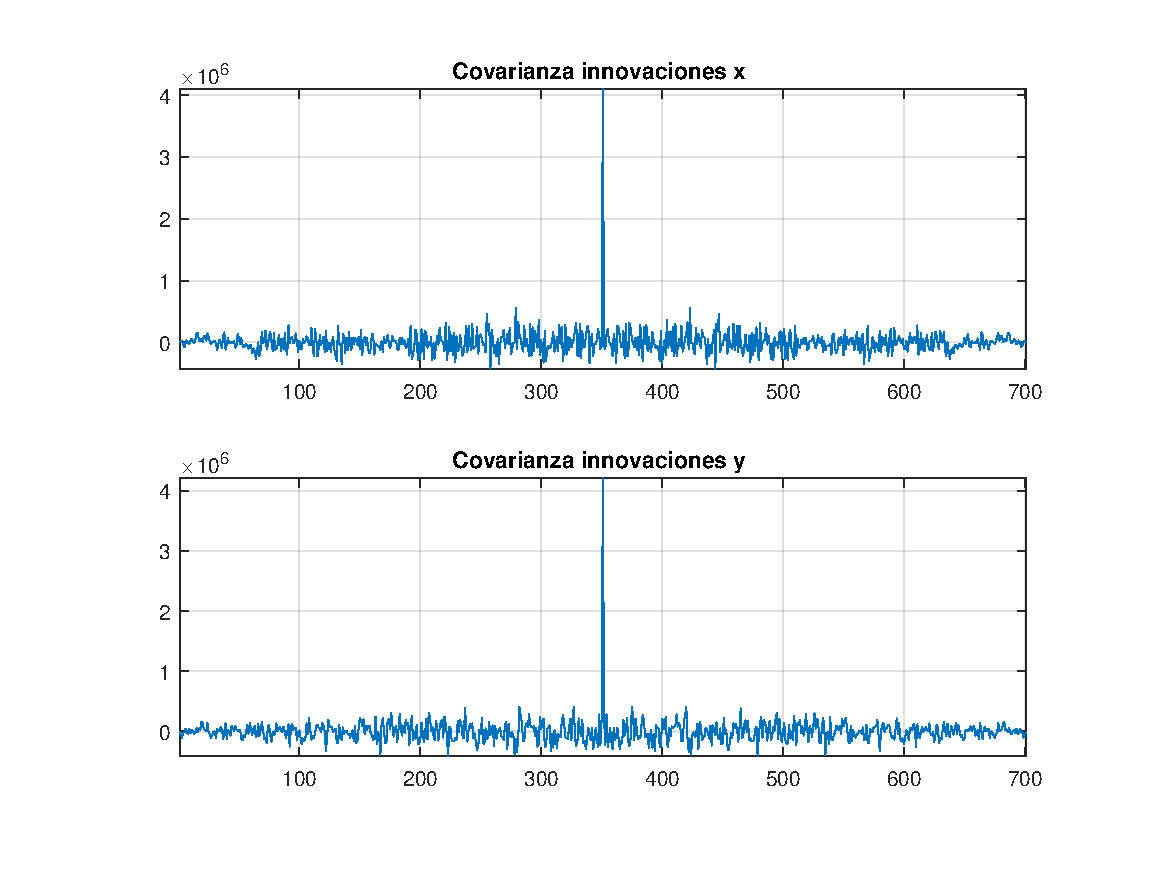
\includegraphics[width=1.0\textwidth,keepaspectratio]{Figuras/covinn_ej4b.pdf}
		\caption{Correlación De Innovaciones}
		\label{fig:ej4b_cov}
	\end{figure}
	
%--------------------------------------------------------------------------------------------------
	
\subsection{Medición de V - Sesgo en V}

	En la Figura \ref{fig:ej4c} se observa el resultado de la estimación. En la misma la estimación no sólo no sigue la trayectoria, sino que se aparta cada vez más de ella a medida que transcurre el tiempo, tanto si se ignora el sesgo, como si se trata de estimarlo (problemas de observabilidad).

	\begin{figure}[H]
		\centering
		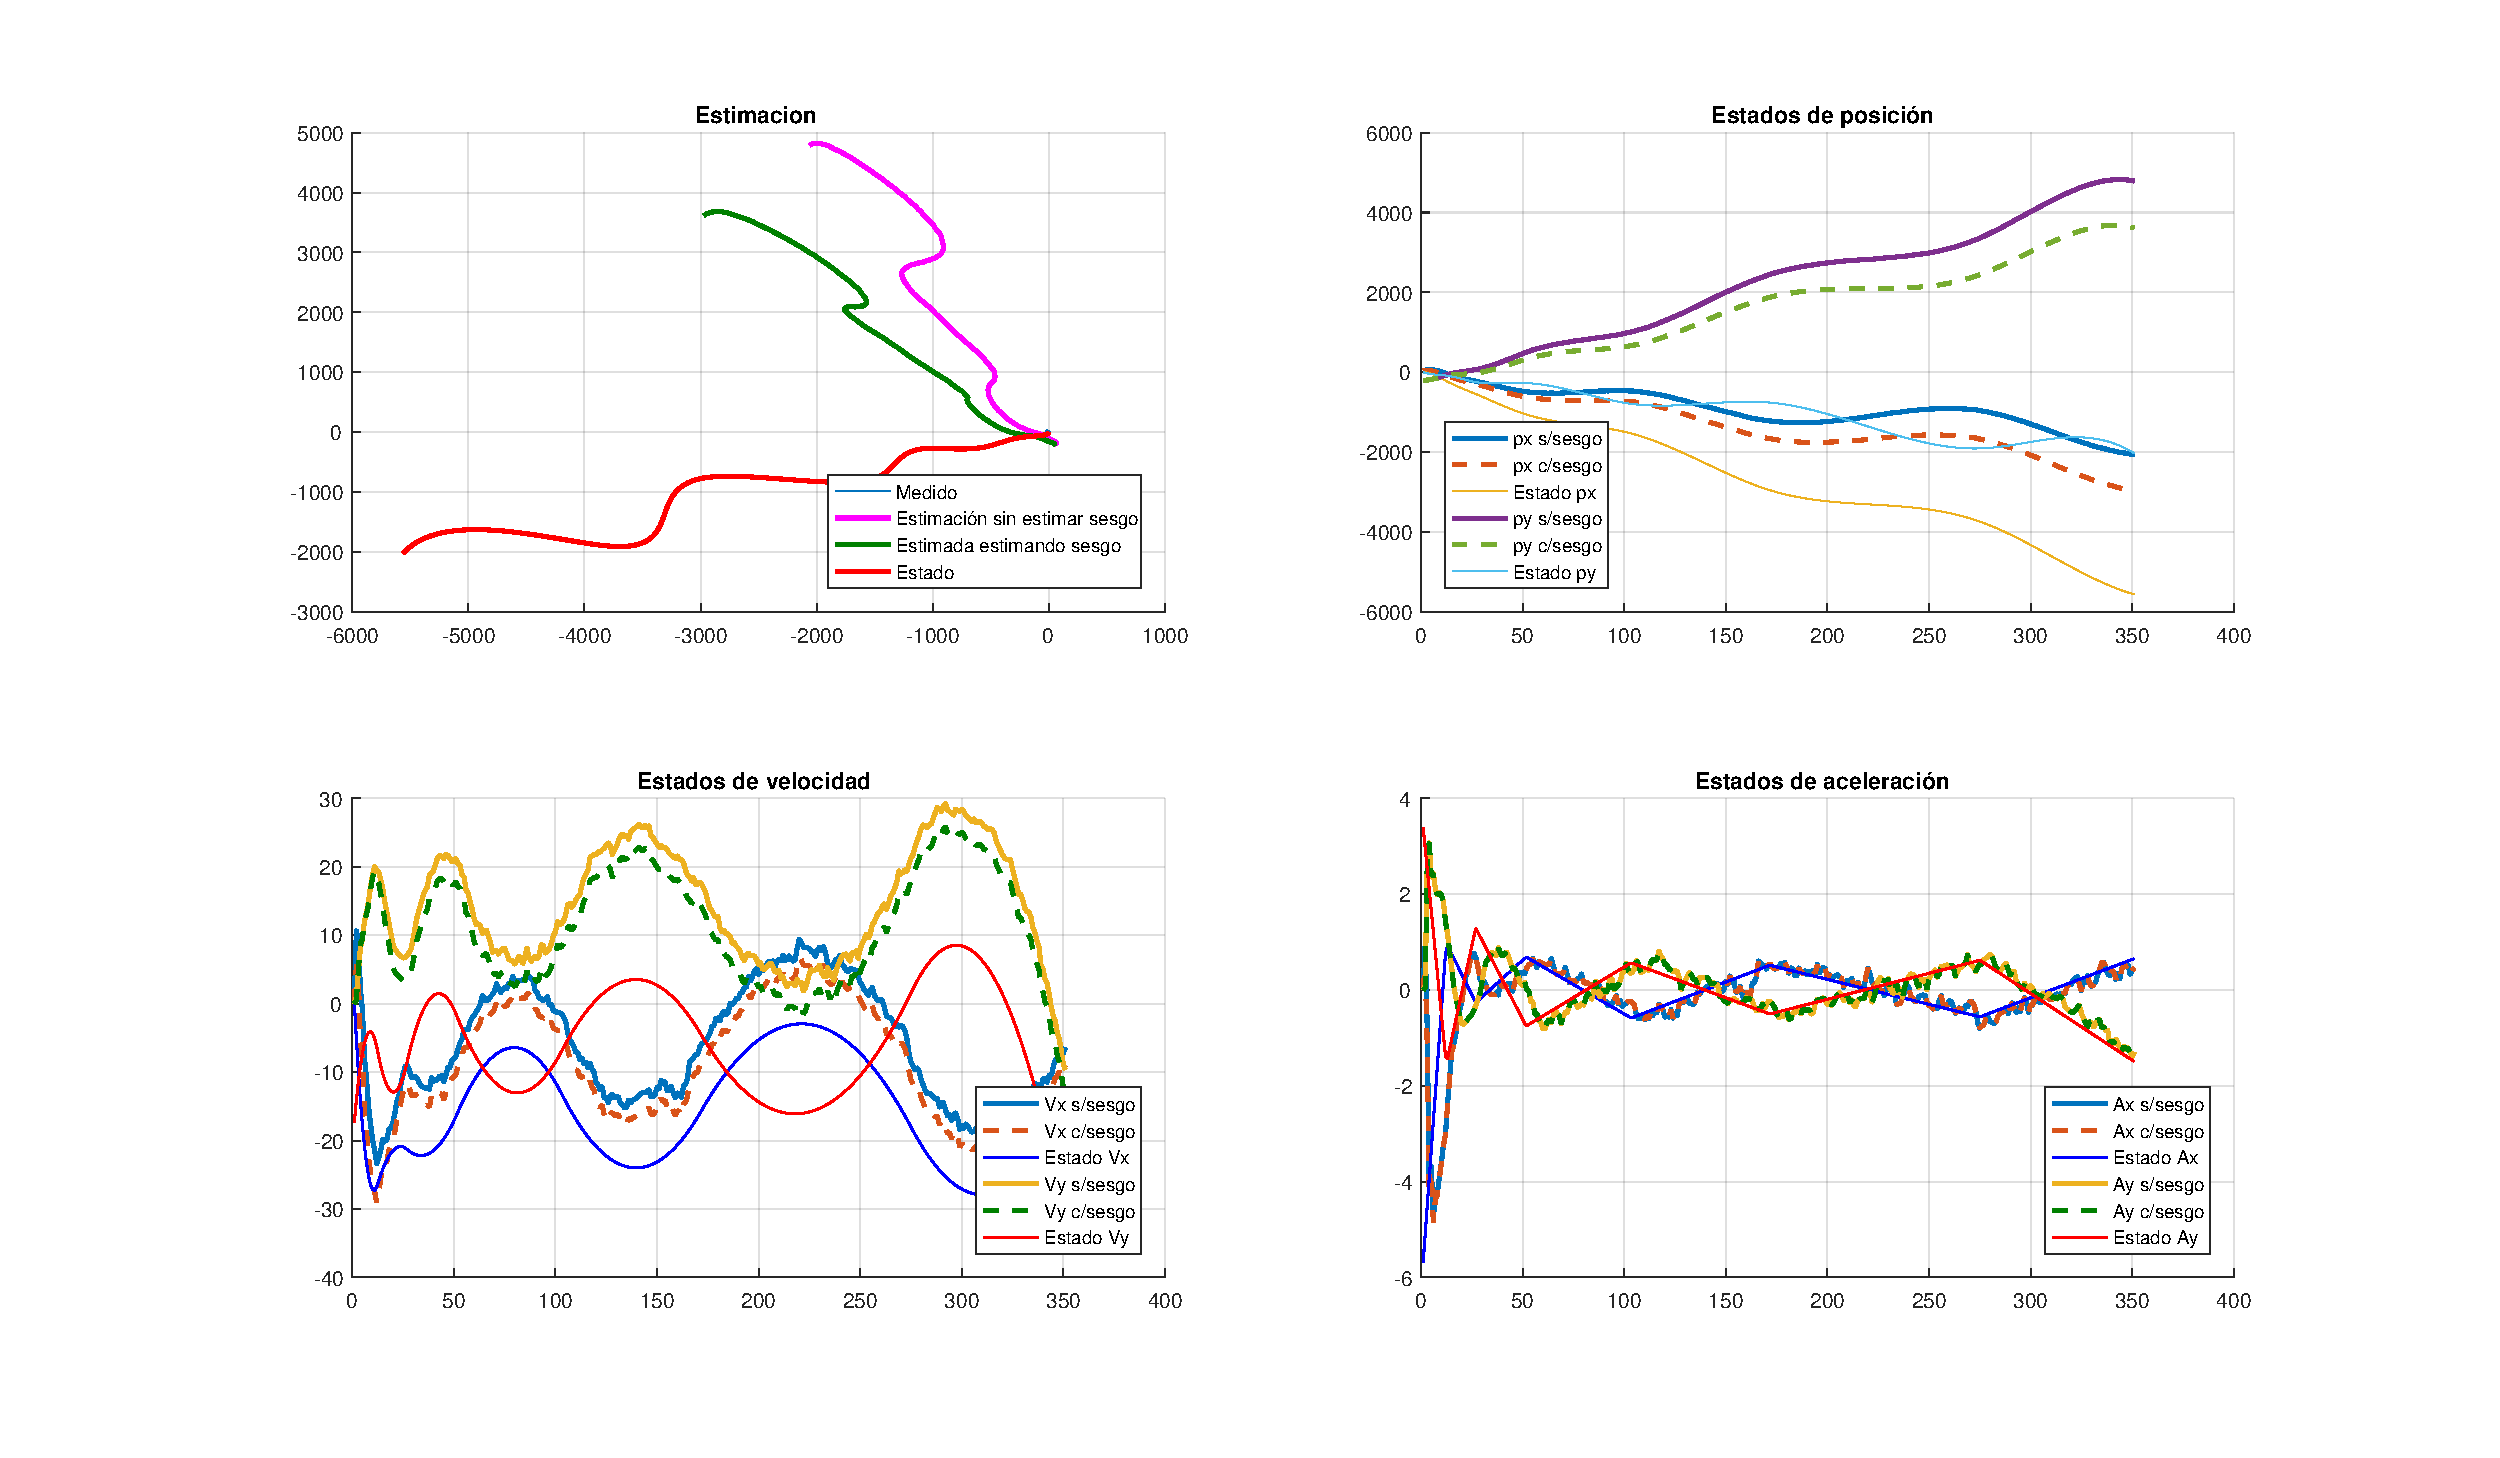
\includegraphics[scale=0.5,trim={6,5cm 0 0 0}]{Figuras/graf_ej4c.pdf}
		\caption{Estimación De Trayectoria}
		\label{fig:ej4c}
	\end{figure}
	
	En la Figura \ref{fig:ej4c_bias} se observa que la estimación del sesgo converge, pero no a los valores correctos como es de esperar.
	
	\begin{figure}[H]
		\centering
		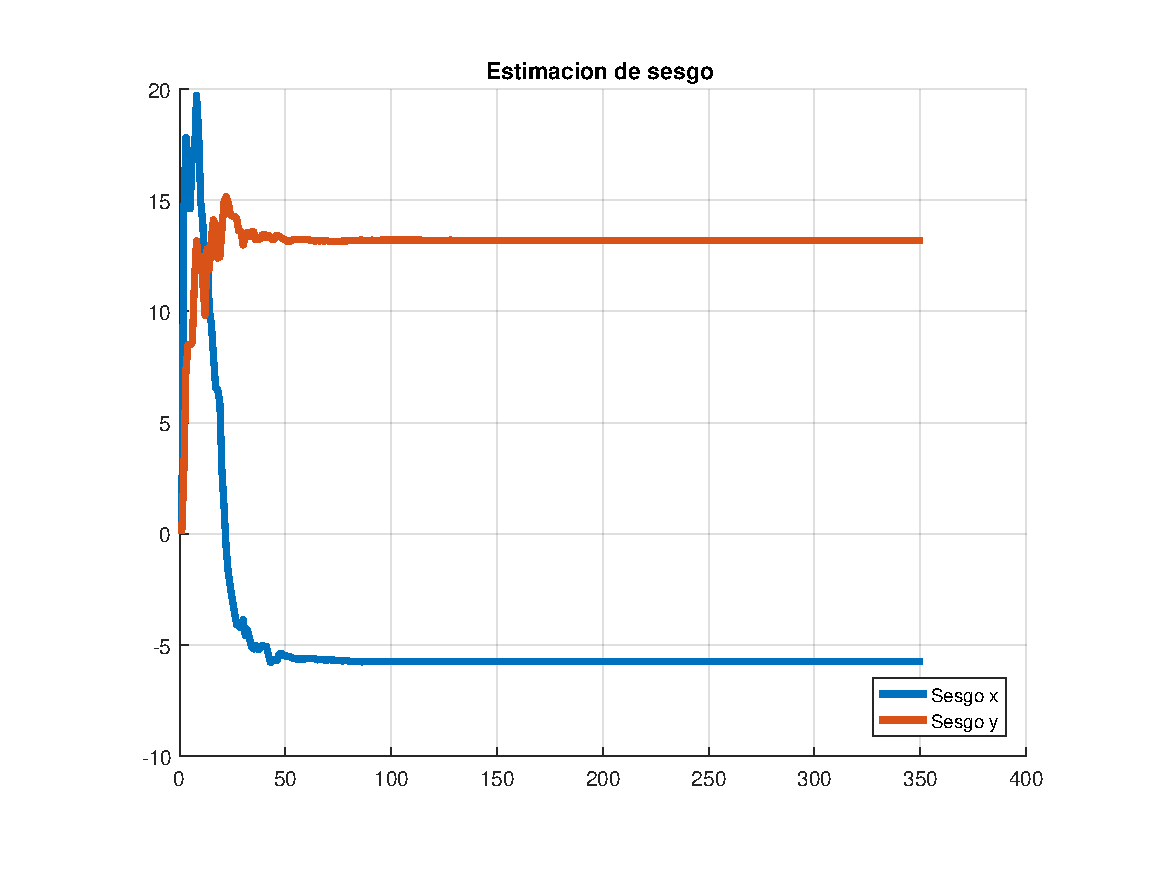
\includegraphics[width=0.7\textwidth,keepaspectratio]{Figuras/bias_ej4c.pdf}
		\caption{Estimación Del Sesgo}
		\label{fig:ej4c_bias}
	\end{figure}
	
	En la Figura \ref{fig:ej4c_cov} se observa la autocorrelación innovaciónes. Es posible ver que el proceso ya no es del todo blanco.
	
	\begin{figure}[H]
		\centering
		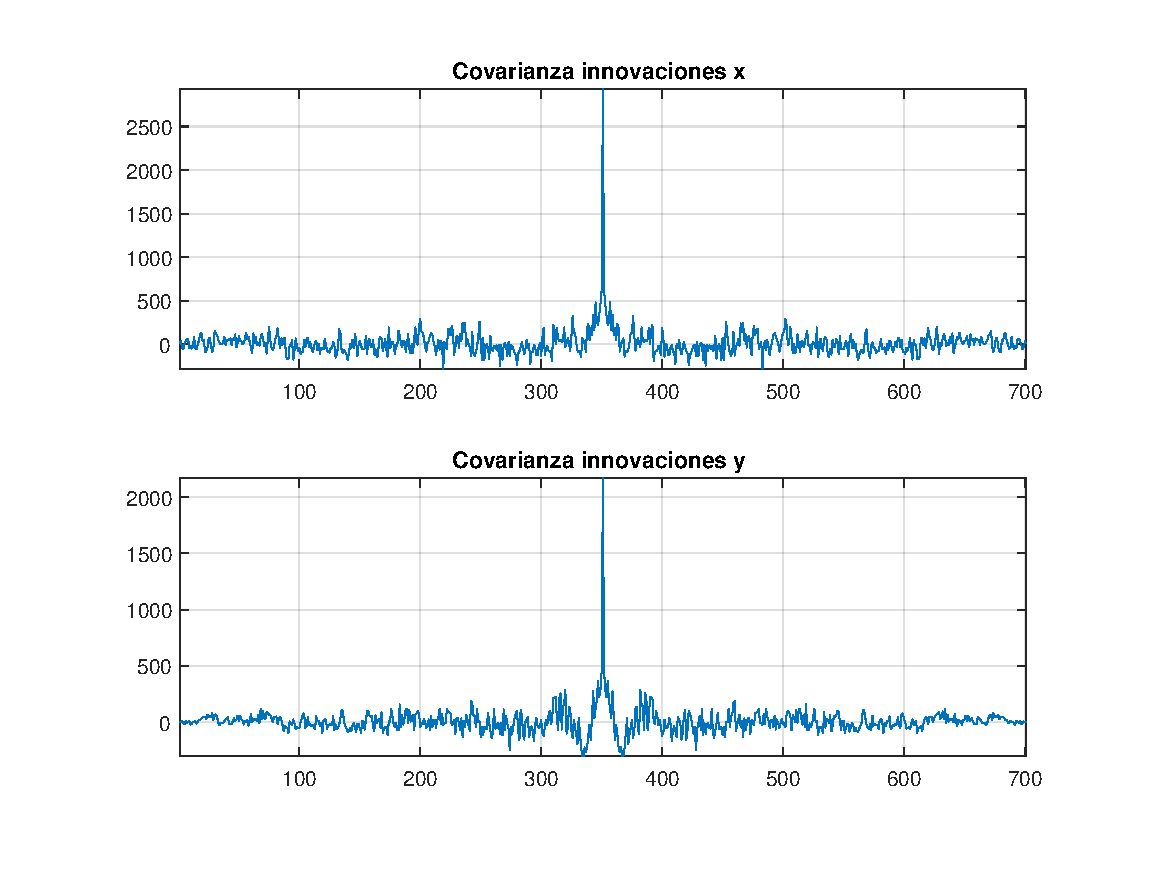
\includegraphics[width=1.0\textwidth,keepaspectratio]{Figuras/covinn_ej4c.pdf}
		\caption{Correlación De Innovaciones}
		\label{fig:ej4c_cov}
	\end{figure}
	
%--------------------------------------------------------------------------------------------------

\subsection{Medición de PVA - Sesgo en V}

	En la Figura \ref{fig:ej4d} puede observarse el resultado de la estimación. En este caso no se tienen problemas de observabilidad, por lo que la estimación sigue la trayectoria y además sigue los valores de velocidad reales.

	\begin{figure}[H]
		\centering
		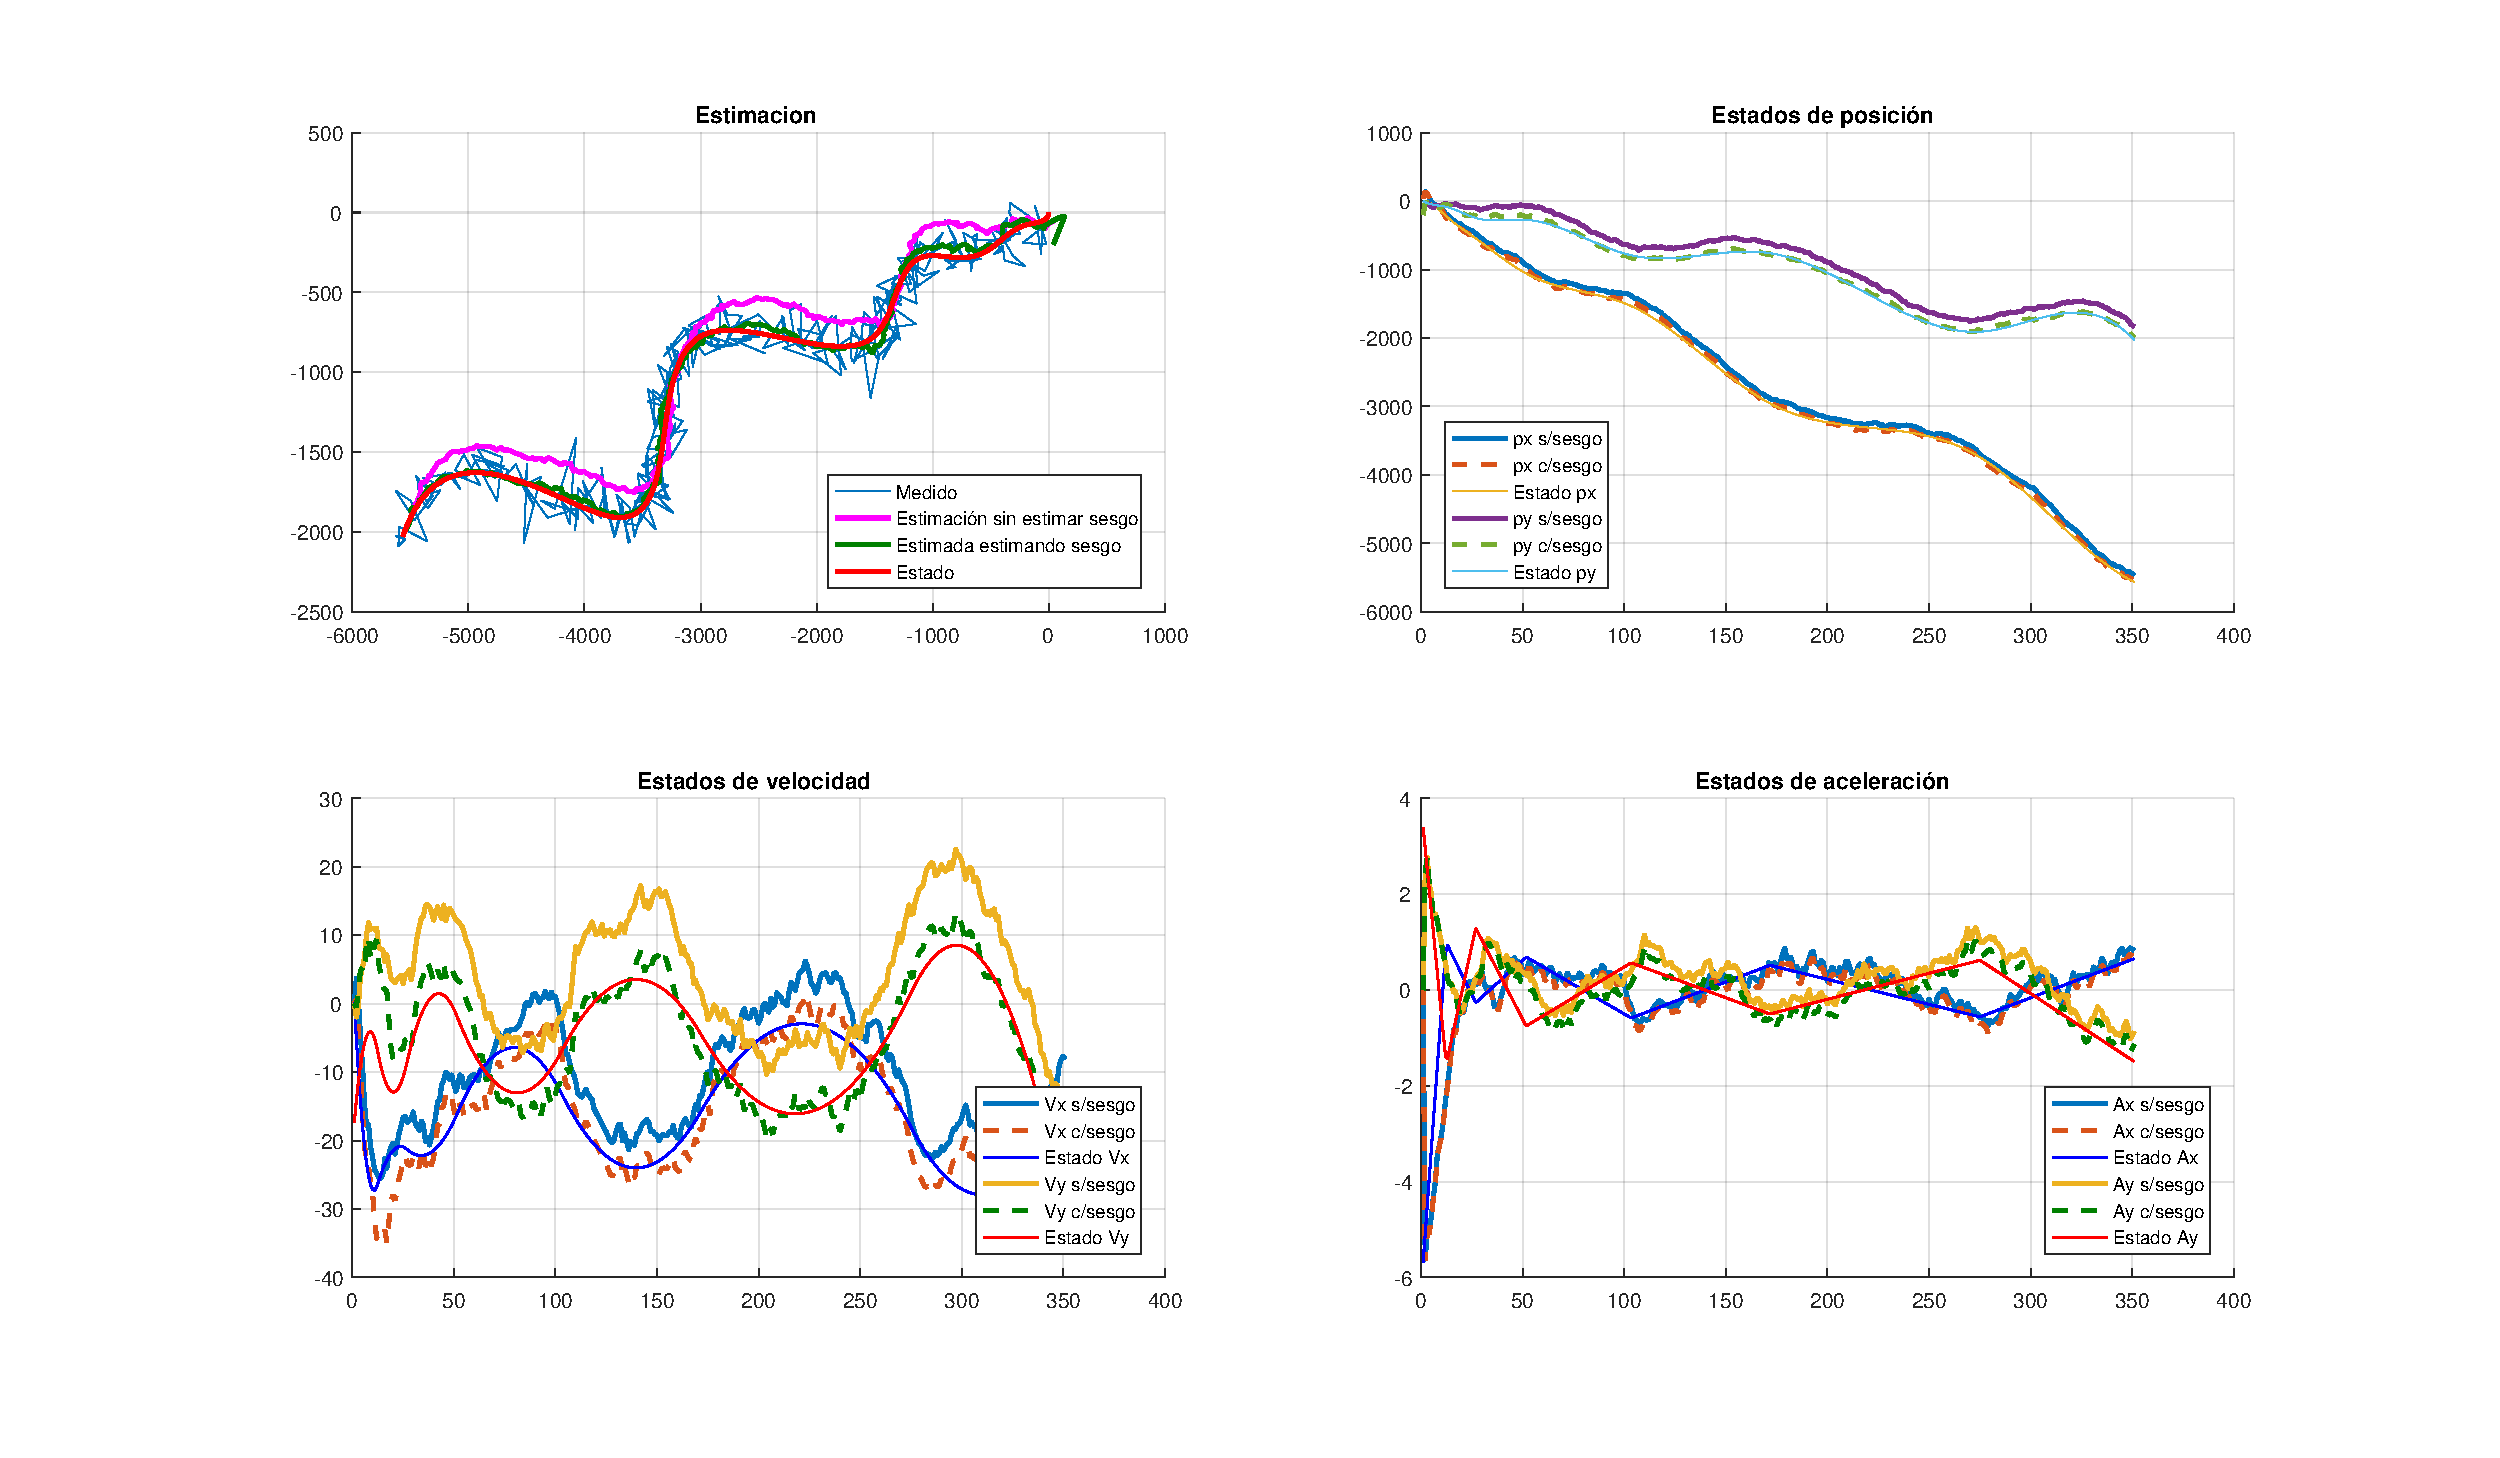
\includegraphics[scale=0.5,trim={6,5cm 0 0 0}]{Figuras/graf_ej4d.pdf}
		\caption{Estimación De Trayectoria}
		\label{fig:ej4d}
	\end{figure}
	
	En la Figura \ref{fig:ej4d_bias} se observa la convergencia de la estimación del sesgo. Al no tener problemas de observabilidad, puede comprobarse que converge a los valores correctos ($\vect{b}_v = [\SI{10}{\m\per\s} \; \SI{20}{\m\per\s}]^T$).
	
	\begin{figure}[H]
		\centering
		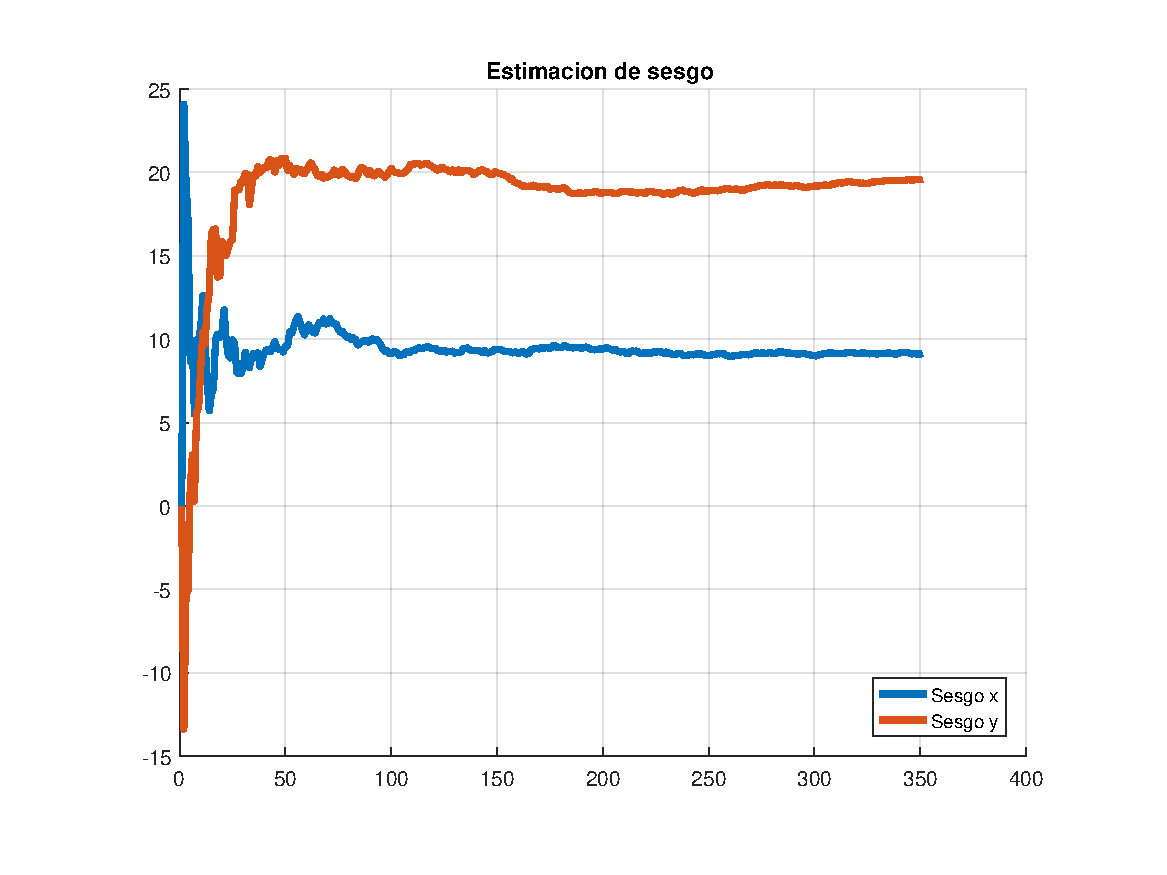
\includegraphics[width=0.7\textwidth,keepaspectratio]{Figuras/bias_ej4d.pdf}
		\caption{Estimación Del Sesgo}
		\label{fig:ej4d_bias}
	\end{figure}
	
	En la Figura \ref{fig:ej4d_cov} se observa la autocorrelación de las innovaciones. Allí puede notarse que ya no es un proceso blanco, a pesar de que se estiman bien los estados.
	
	\begin{figure}[H]
		\centering
		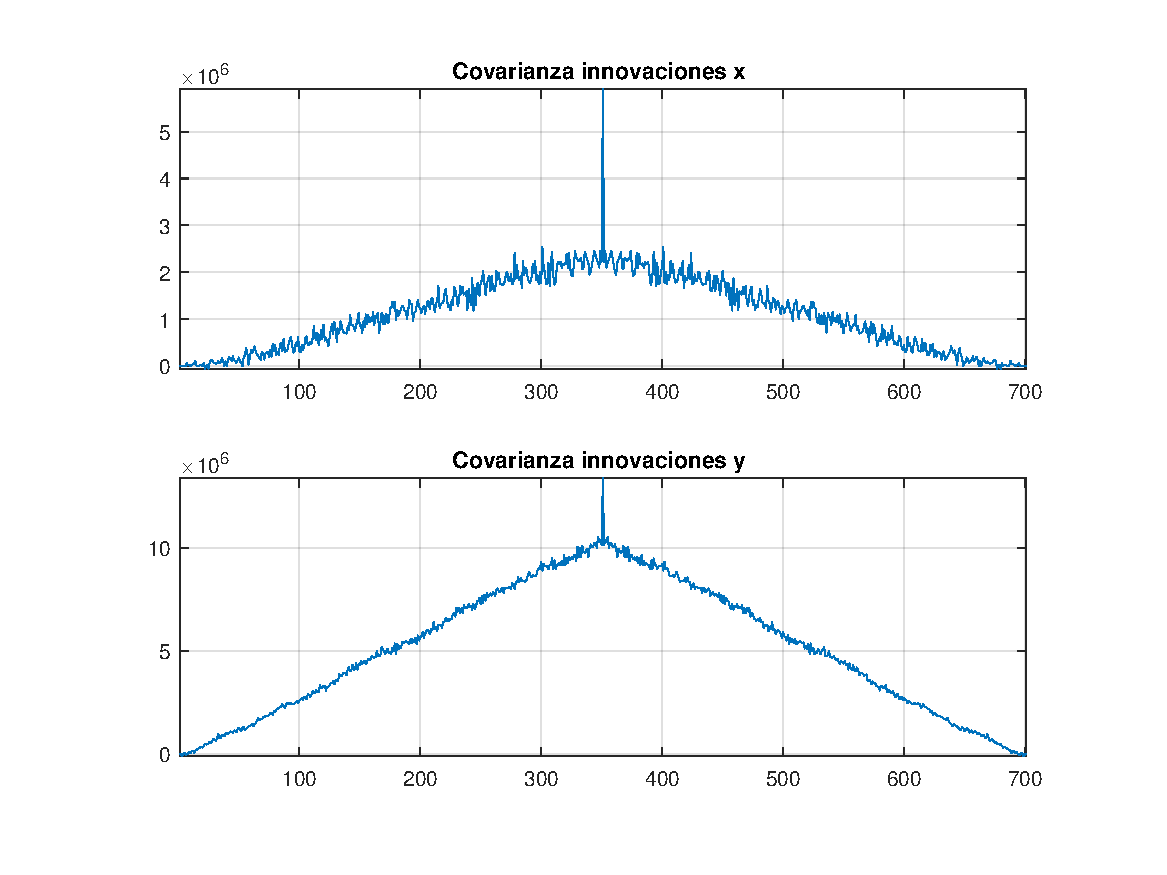
\includegraphics[width=1.0\textwidth,keepaspectratio]{Figuras/covinn_ej4d.pdf}
		\caption{Correlación De Innovaciones}
		\label{fig:ej4d_cov}
	\end{figure}

%--------------------------------------------------------------------------------------------------

\subsection{Medición de A - Sesgo en A}

	En la Figura \ref{fig:ej4e} podemos observar el resultado de la estimación. En este caso no se tiene observabilidad, por lo que el resultado empeora cada vez más a medida que pasa el tiempo.

	\begin{figure}[H]
		\centering
		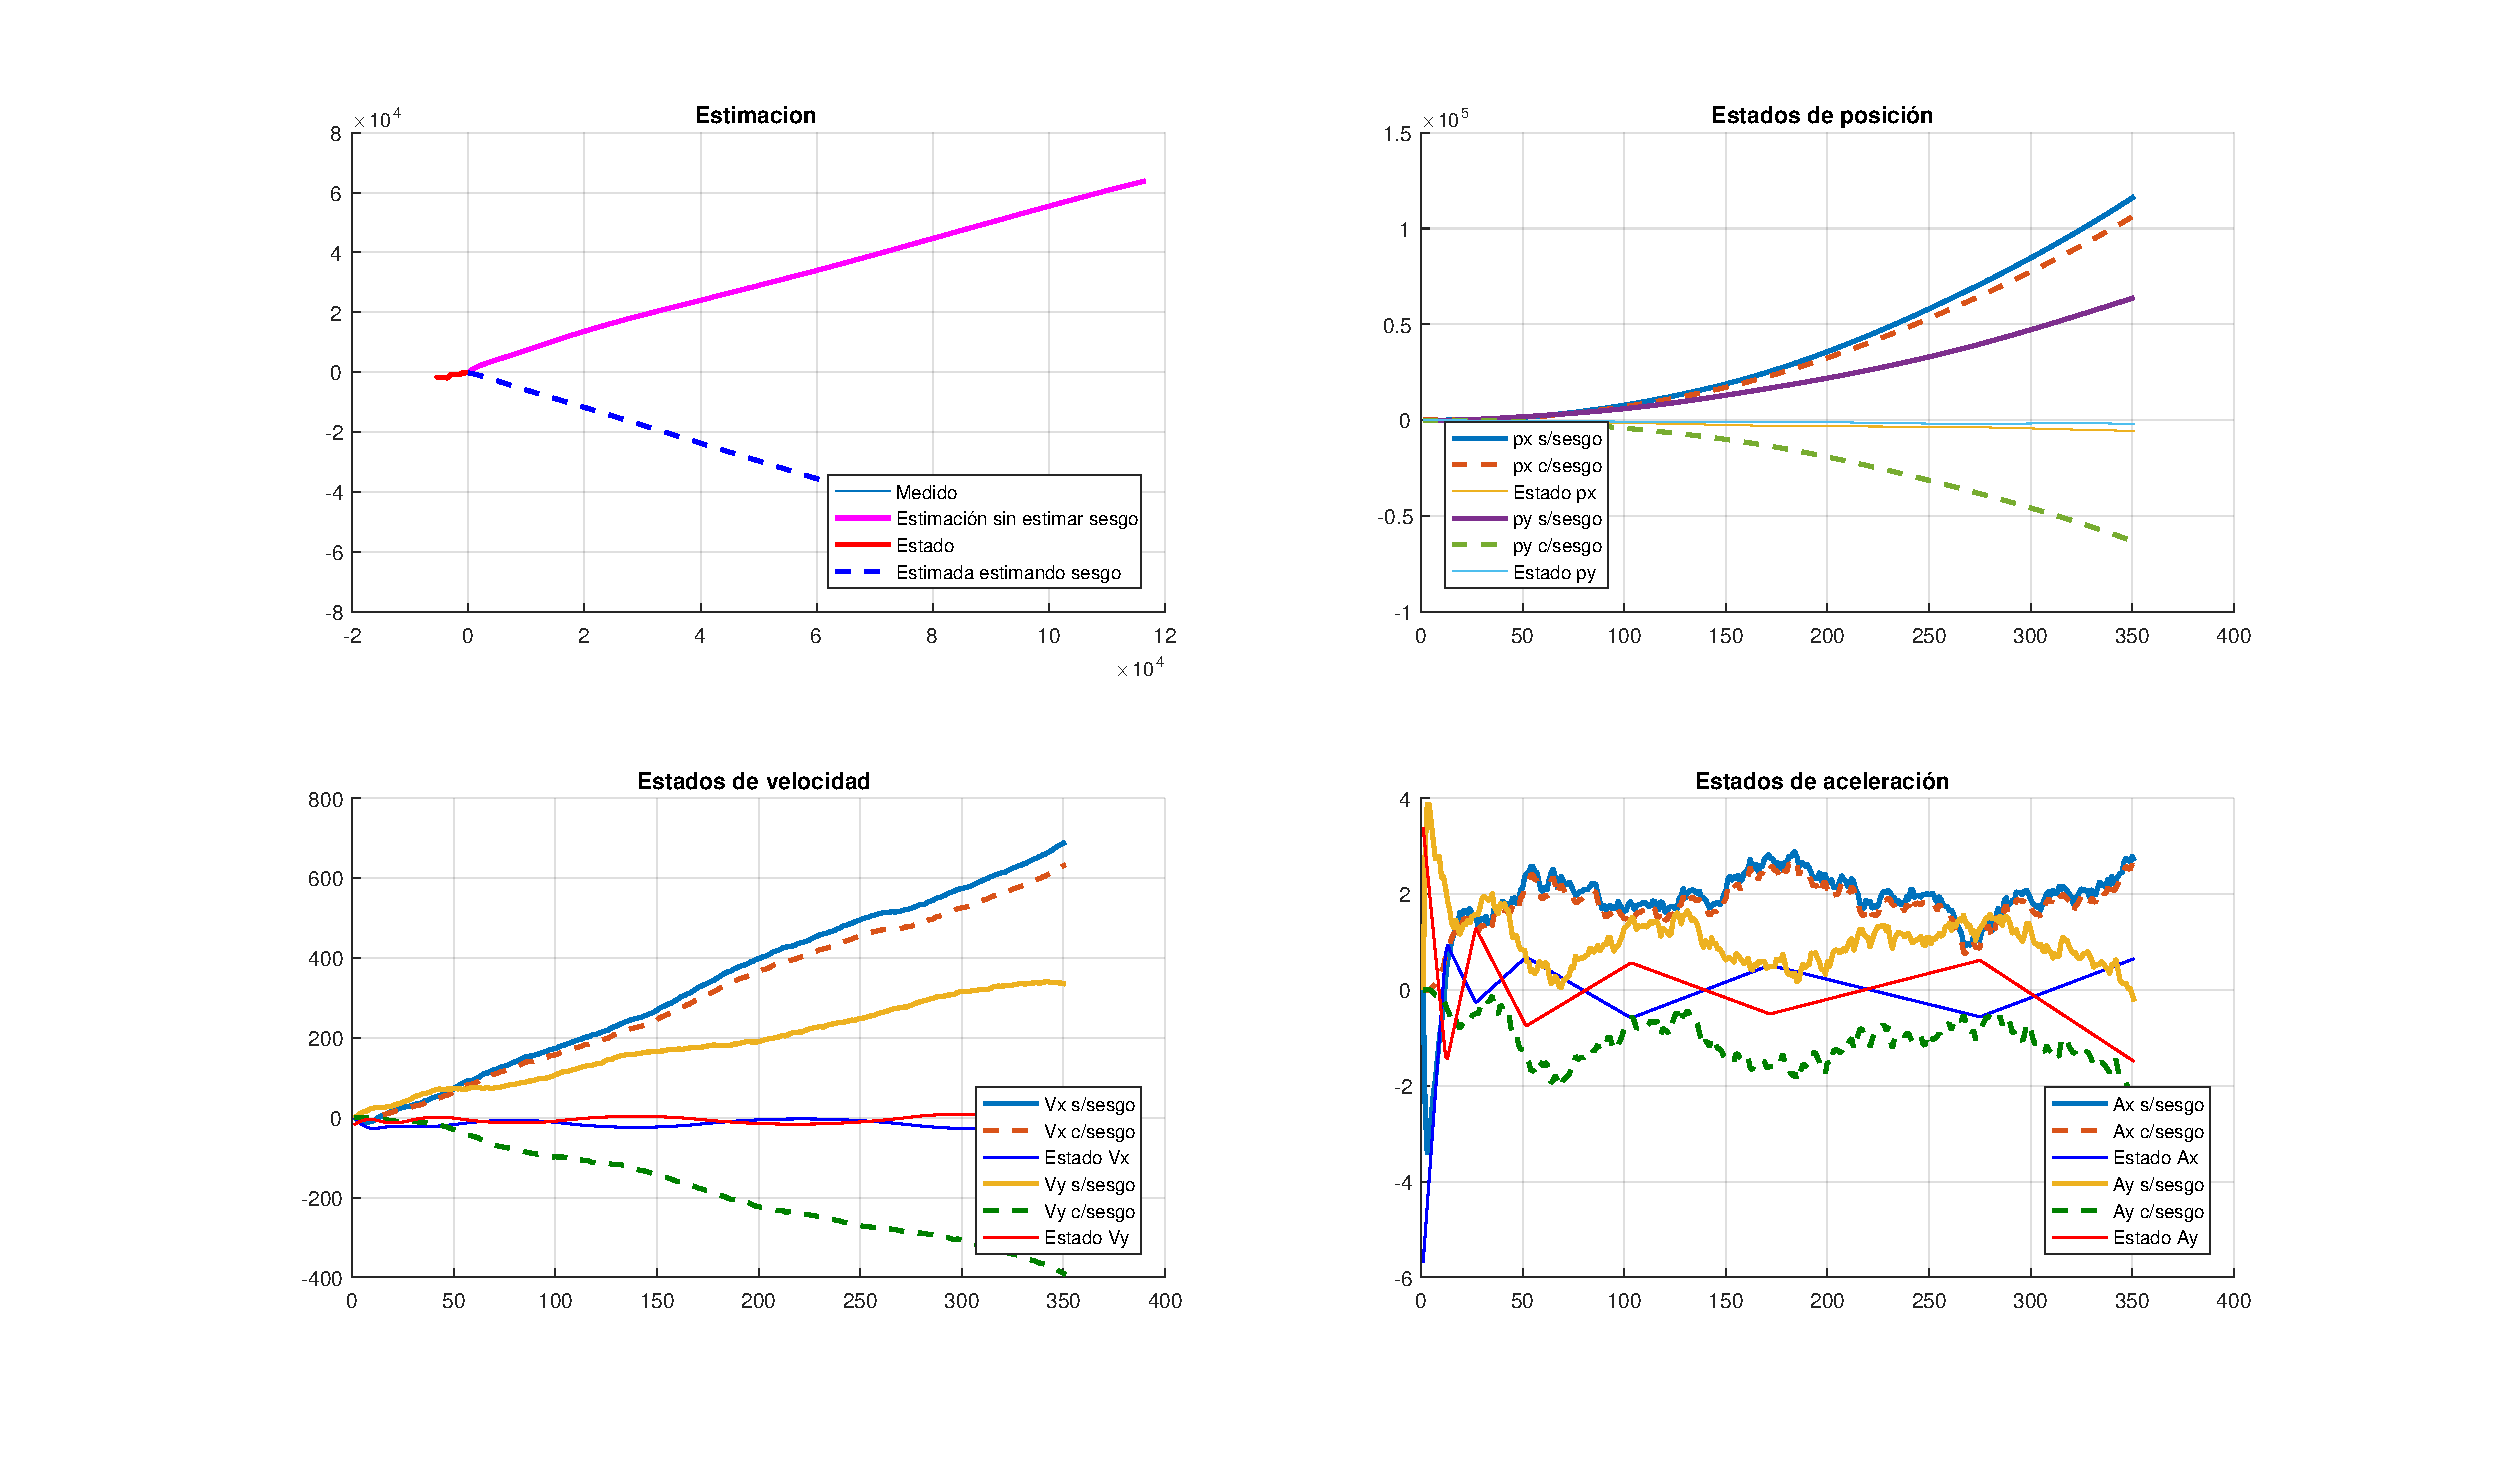
\includegraphics[scale=0.5,trim={6,5cm 0 0 0}]{Figuras/graf_ej4e.pdf}
		\caption{Estimación De Trayectoria}
		\label{fig:ej4e}
	\end{figure}
	
	En la Figura \ref{fig:ej4e_bias} podemos observar la convergencia de la estimación. Si bien la misma converge, al no tener observabilidad no lo hace a los valores correctos.
	
	\begin{figure}[H]
		\centering
		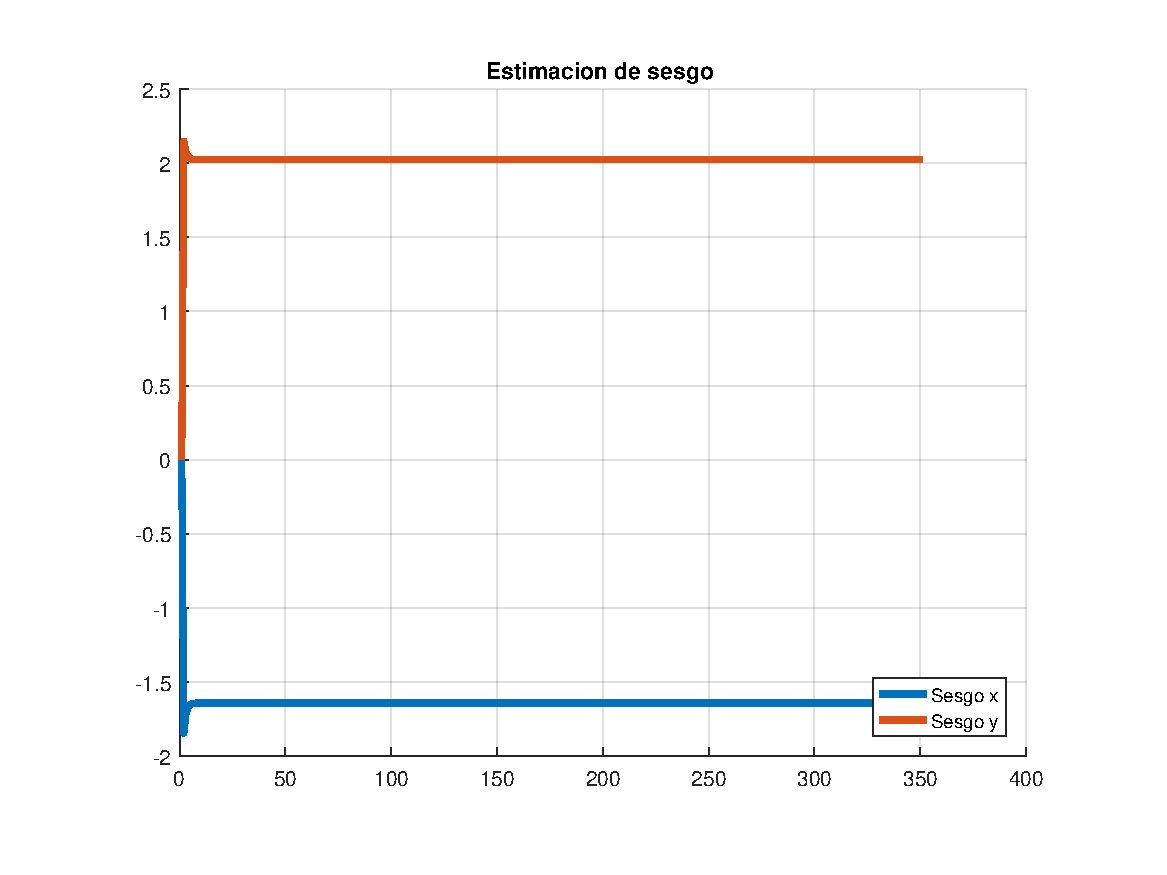
\includegraphics[width=0.7\textwidth,keepaspectratio]{Figuras/bias_ej4e.pdf}
		\caption{Estimación Del Sesgo}
		\label{fig:ej4e_bias}
	\end{figure}
	
	En la Figura \ref{fig:ej4e_cov} observamos la autocorrelación de las innovaciones. Puede verse que no se trata de un proceso totalmente blanco.
	
	\begin{figure}[H]
		\centering
		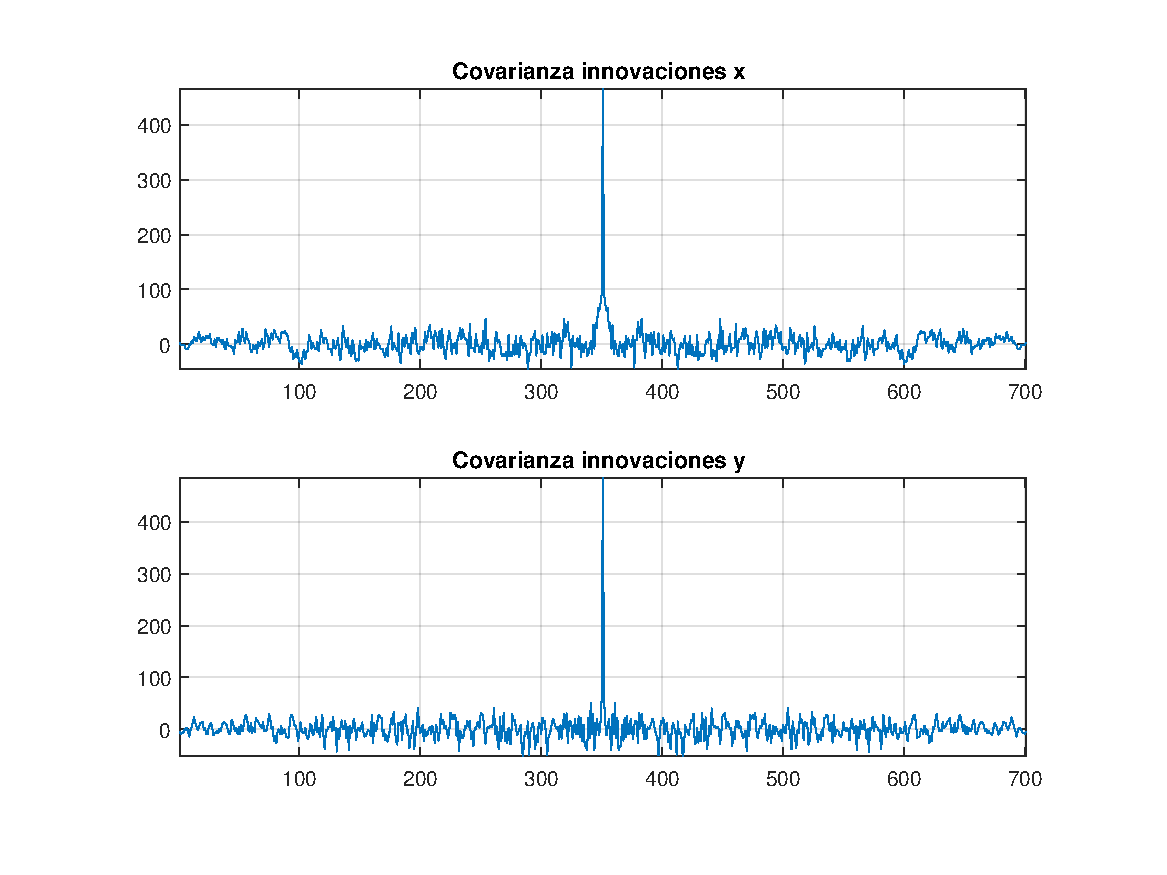
\includegraphics[width=1.0\textwidth,keepaspectratio]{Figuras/covinn_ej4e.pdf}
		\caption{Correlación De Innovaciones}
		\label{fig:ej4e_cov}
	\end{figure}

%--------------------------------------------------------------------------------------------------

\subsection{Medición de PVA - Sesgo en A}

	En la Figura \ref{fig:ej3f} se observa el resultado de la estimación. Nuevamente no se tienen problemas de observabilidad, por lo que la estimación sigue la trayectoria y, además, sigue la aceleración de forma correcta.

	\begin{figure}[H]
		\centering
		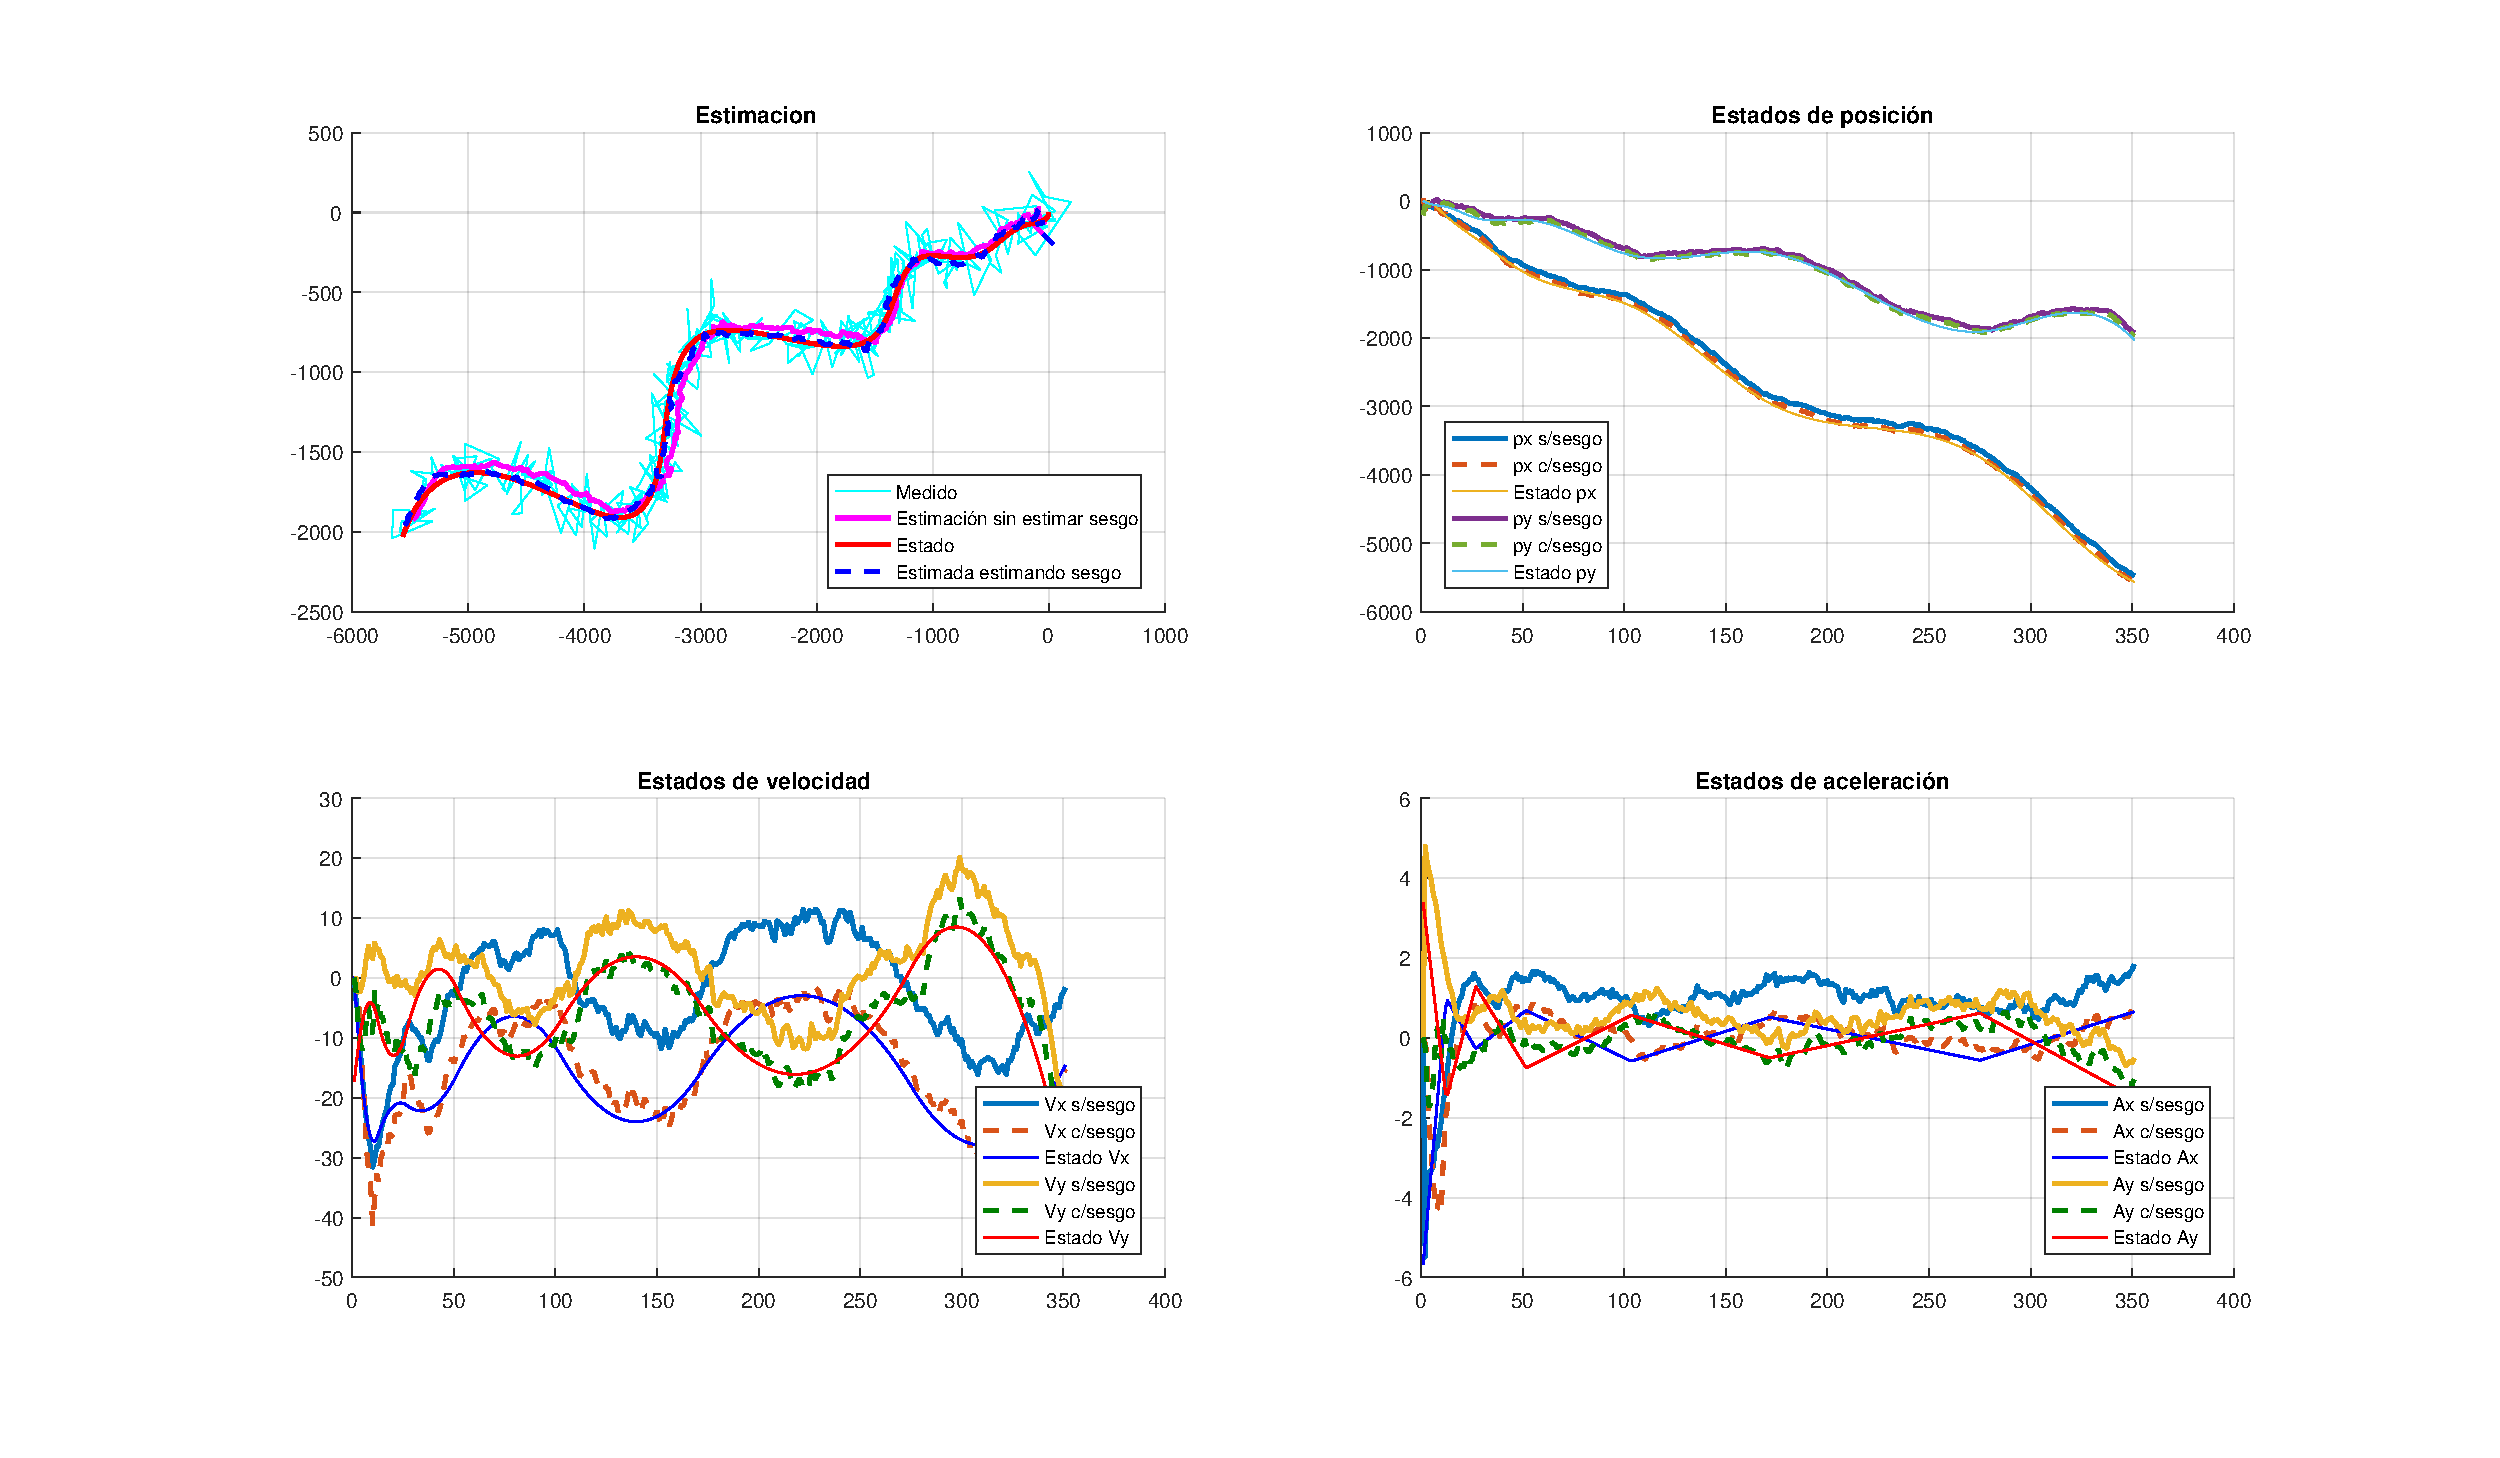
\includegraphics[scale=0.5,trim={6,5cm 0 0 0}]{Figuras/graf_ej4f.pdf}
		\caption{Estimación De Trayectoria}
		\label{fig:ej3f}
	\end{figure}
	
	En la Figura \ref{fig:ej3f_bias} se observa la convergencia de la estimación del sesgo. Al tener observabilidad, puede comprobarse que converge a los valores correctos ($\vect{b}_a = [\SI{1}{\m\per\s\squared} \; \SI{2}{\m\per\s\squared}]^T$).
	
	\begin{figure}[H]
		\centering
		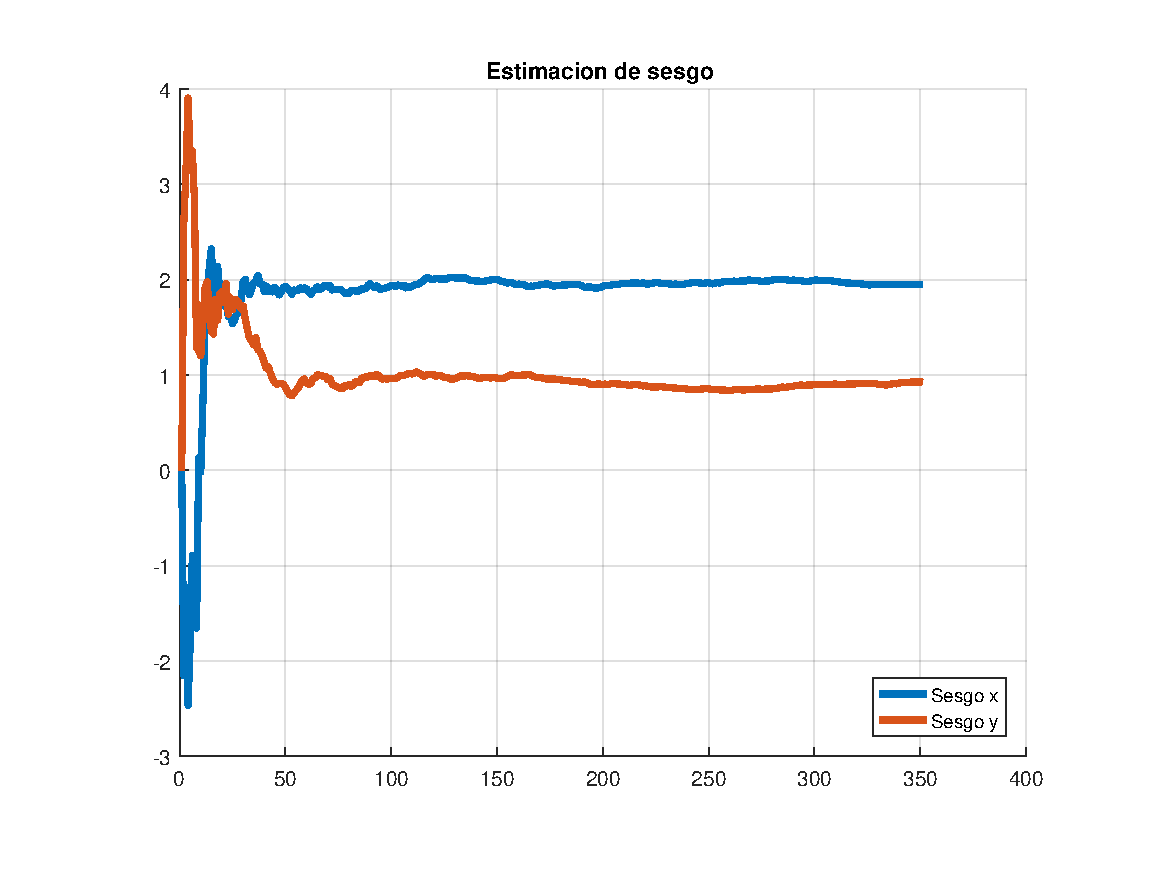
\includegraphics[width=0.7\textwidth,keepaspectratio]{Figuras/bias_ej4f.pdf}
		\caption{Estimación Del Sesgo}
		\label{fig:ej3f_bias}
	\end{figure}
	
	En la Figura \ref{fig:ej3f_cov} se observa la autocorrelación de las innovaciones. Puede verse que no se trata de un proceso blanco.

	\begin{figure}[H]
		\centering
		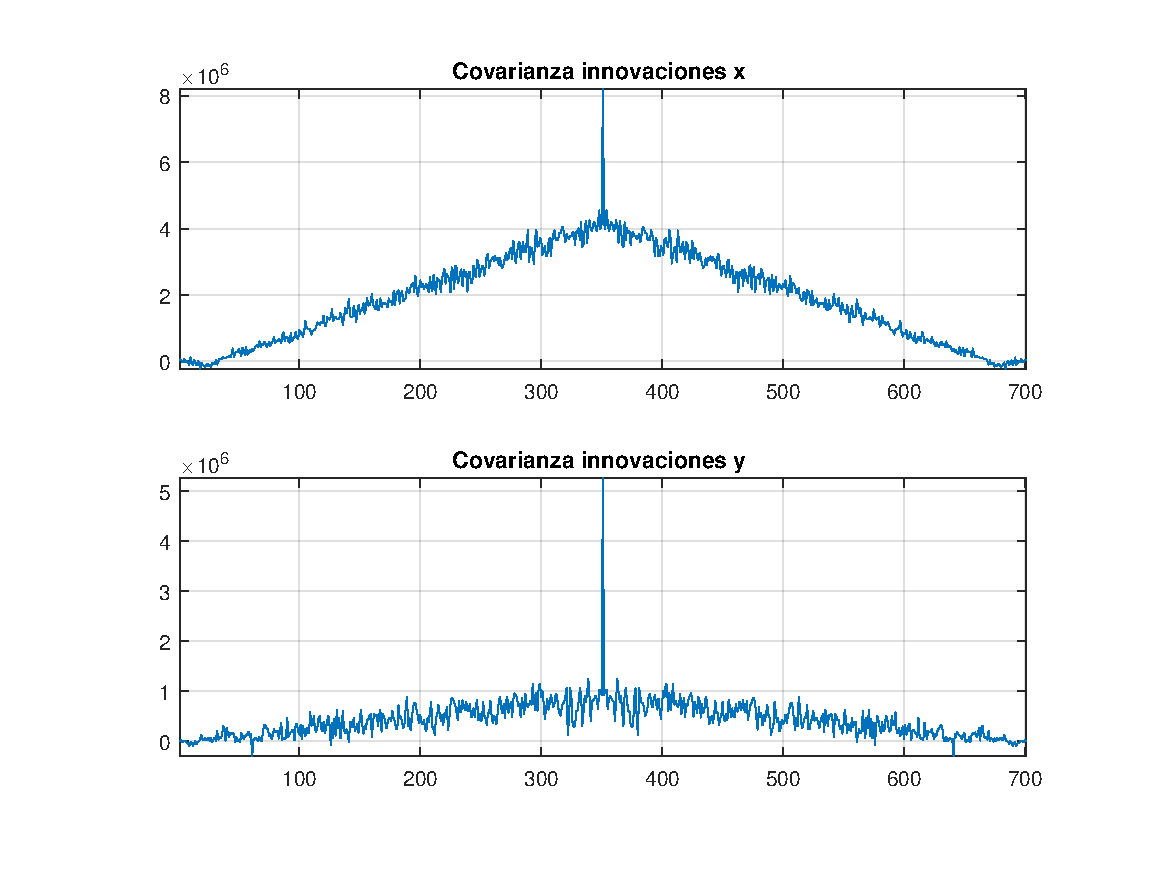
\includegraphics[width=1.0\textwidth,keepaspectratio]{Figuras/covinn_ej4f.pdf}
		\caption{Correlación De Innovaciones}
		\label{fig:ej3f_cov}
	\end{figure}
	
%--------------------------------------------------------------------------------------------------

	\subsection{Test de observabilidad}

	Al realizar el test de observabilidad a los 6 casos anteriores se obtiene la siguiente tabla que lo resume:

		\begin{table}[h!]
			\centering
			\begin{tabular}{cccc}
				\toprule
				Medición	& Sesgo		& Cantidad no observables	& Observables\\
				\midrule
				$\vect{p}$	& $\vect{b}_p$	& 2				& $\vect{p}$ $\vect{v}$ $\vect{a}$\\
				$\vect{p}$ $\vect{v}$ $\vect{a}$	& $\vect{b}_p$	& 2				& $\vect{p}$ $\vect{v}$ $\vect{a}$\\
				$\vect{v}$	& $\vect{b}_v$	& 4				& $\vect{v}$ $\vect{a}$ \\
			$\vect{p}$ $\vect{v}$ $\vect{a}$	& $\vect{b}_v$	& 0				& $\vect{p}$ $\vect{v}$ $\vect{a}$ $\vect{b}_v$ \\
				$\vect{a}$	& $\vect{b}_a$	& 6				& $\vect{a}$\\
			$\vect{p}$ $\vect{v}$ $\vect{a}$	& $\vect{b}_a$	& 0				& $\vect{p}$ $\vect{v}$ $\vect{a}$ $\vect{b}_a$ \\

				\bottomrule
			\end{tabular}
				\caption{Test de observabilidad para el ejercicio 4.}
				\label{tab:obs_ej2}
		\end{table}



\subsection{Script}

A continuación se incluye el script que realiza la estimación. Puede seleccionarse mediante las variables \texttt{bool\_p}, \texttt{bool\_v}, \texttt{bool\_a}, en 1 o en 0, qué se va a medir. Por otro lado puede seleccionarse mediante las variables \texttt{bool\_pb}, \texttt{bool\_vb}, \texttt{bool\_ab}, en 1 o en 0, en qué variables se desea tener sesgo.
	
	\lstinputlisting[firstline=20, firstnumber=20, lastline=28]{EJ4a.m}
	\lstinputlisting[firstline=130, firstnumber=130, lastline=180]{EJ4a.m}

%--------------------------------------------------------------------------------------------------


	\section{Ejercicio 5 \\ Diferencias Entre Las Estimaciones Según Magnitud De $R$}\label{sec:ej5}
		
	El filtro de Kalman obtiene la mejor estimación en el sentido del error cuadrático medio. Esto quiere decir que cuanto mayor sea la varianza de el ruido de proceso, mas importancia le dará a las mediciones. De la misma manera, cuanto mayor sea la varianza del ruido de medición, mayor importancia le dará al modelo en el espacio de estados para poder realizar la estimación. El objetivo de este punto es ver como se modifica la estimación modificando la magnitud de la matriz de covarianza del ruido de proceso.
	
	En las figuras \ref{fig:ej5r1} y \ref{fig:ej5r2} se observan las estimaciones de las trayectoras para una matriz de covarianza del ruido de proceso $100$ veces mayor y $100$ veces menor a la original, respectivamente. Puede observarse que en el caso de la matriz mayor, el algoritmo le da menos importancia al modelo, y mas a las mediciones. De esta manera, se deja llevar mas por las mediciones y la variabilidad de la trayectoria respecto de la real es mayor que en el caso en que se usa una matriz menor.
	
	\begin{figure}[H]
		\centering
		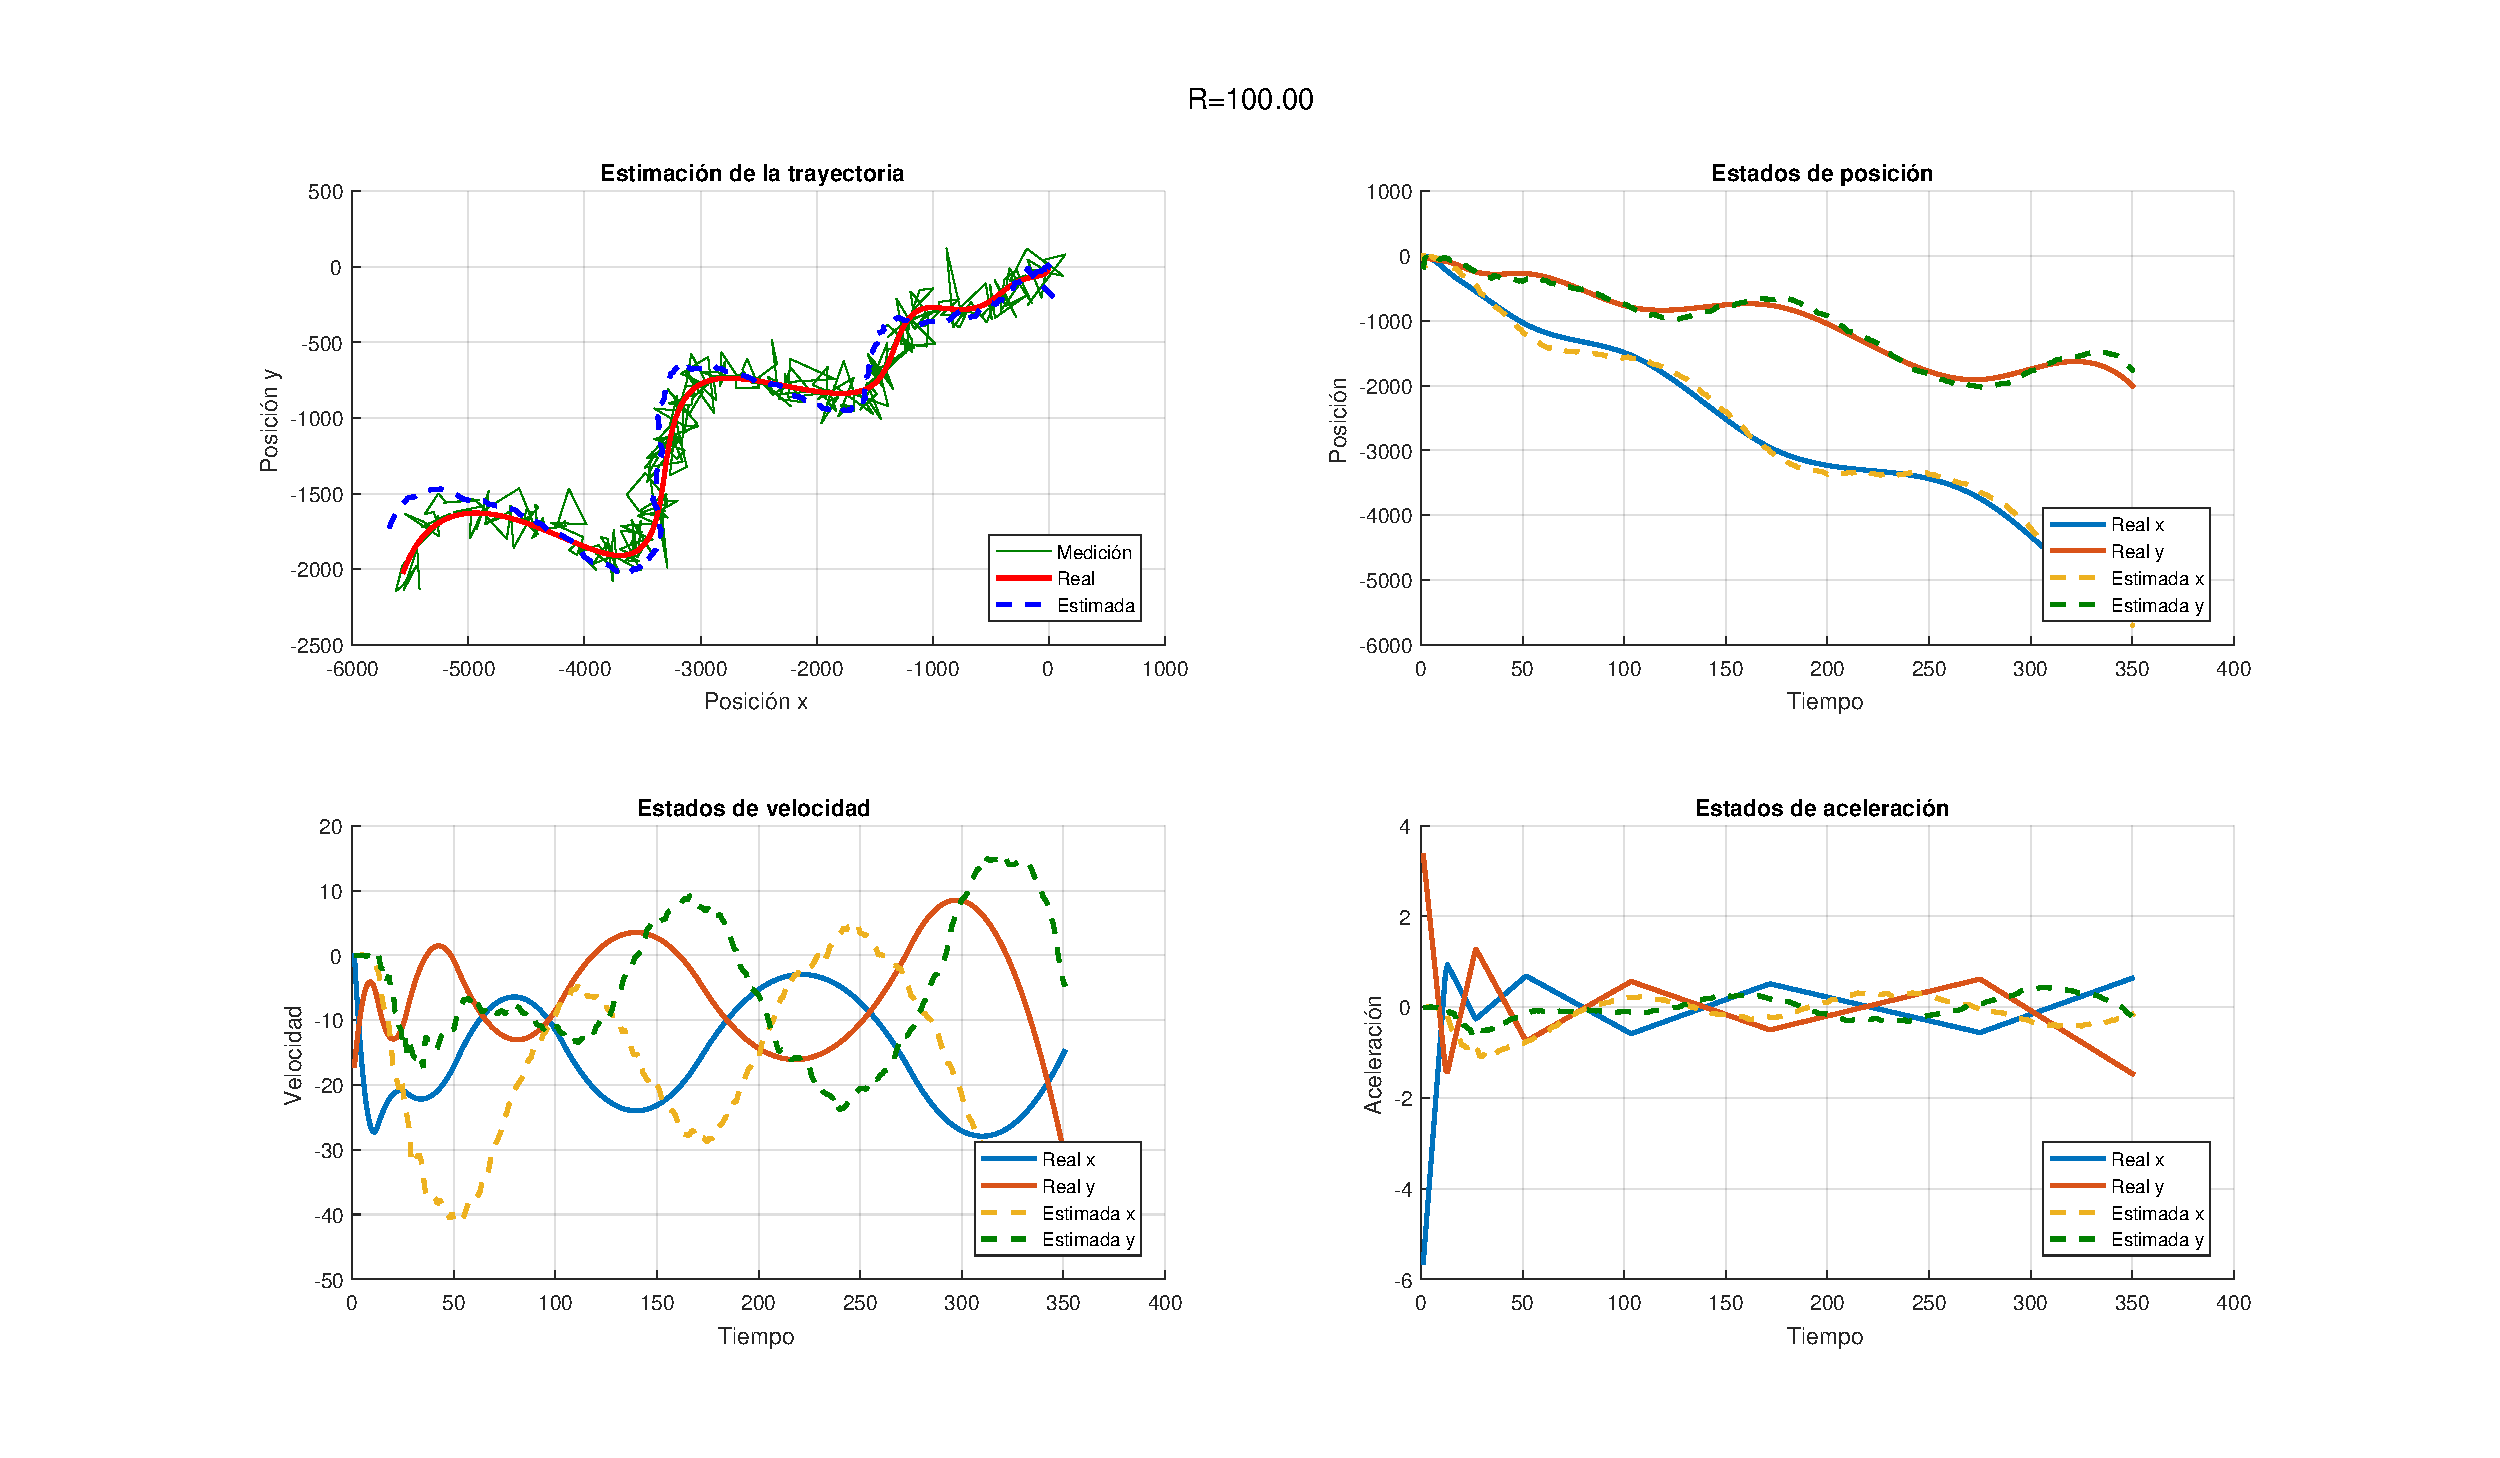
\includegraphics[width=1.0\textwidth,keepaspectratio]{Figuras/graf_ej6_R1.pdf}
		\caption{Estimación de Trayectoria - Matriz de Covarianza Mayor}
		\label{fig:ej5r1}
	\end{figure}
	
	\begin{figure}[H]
		\centering
		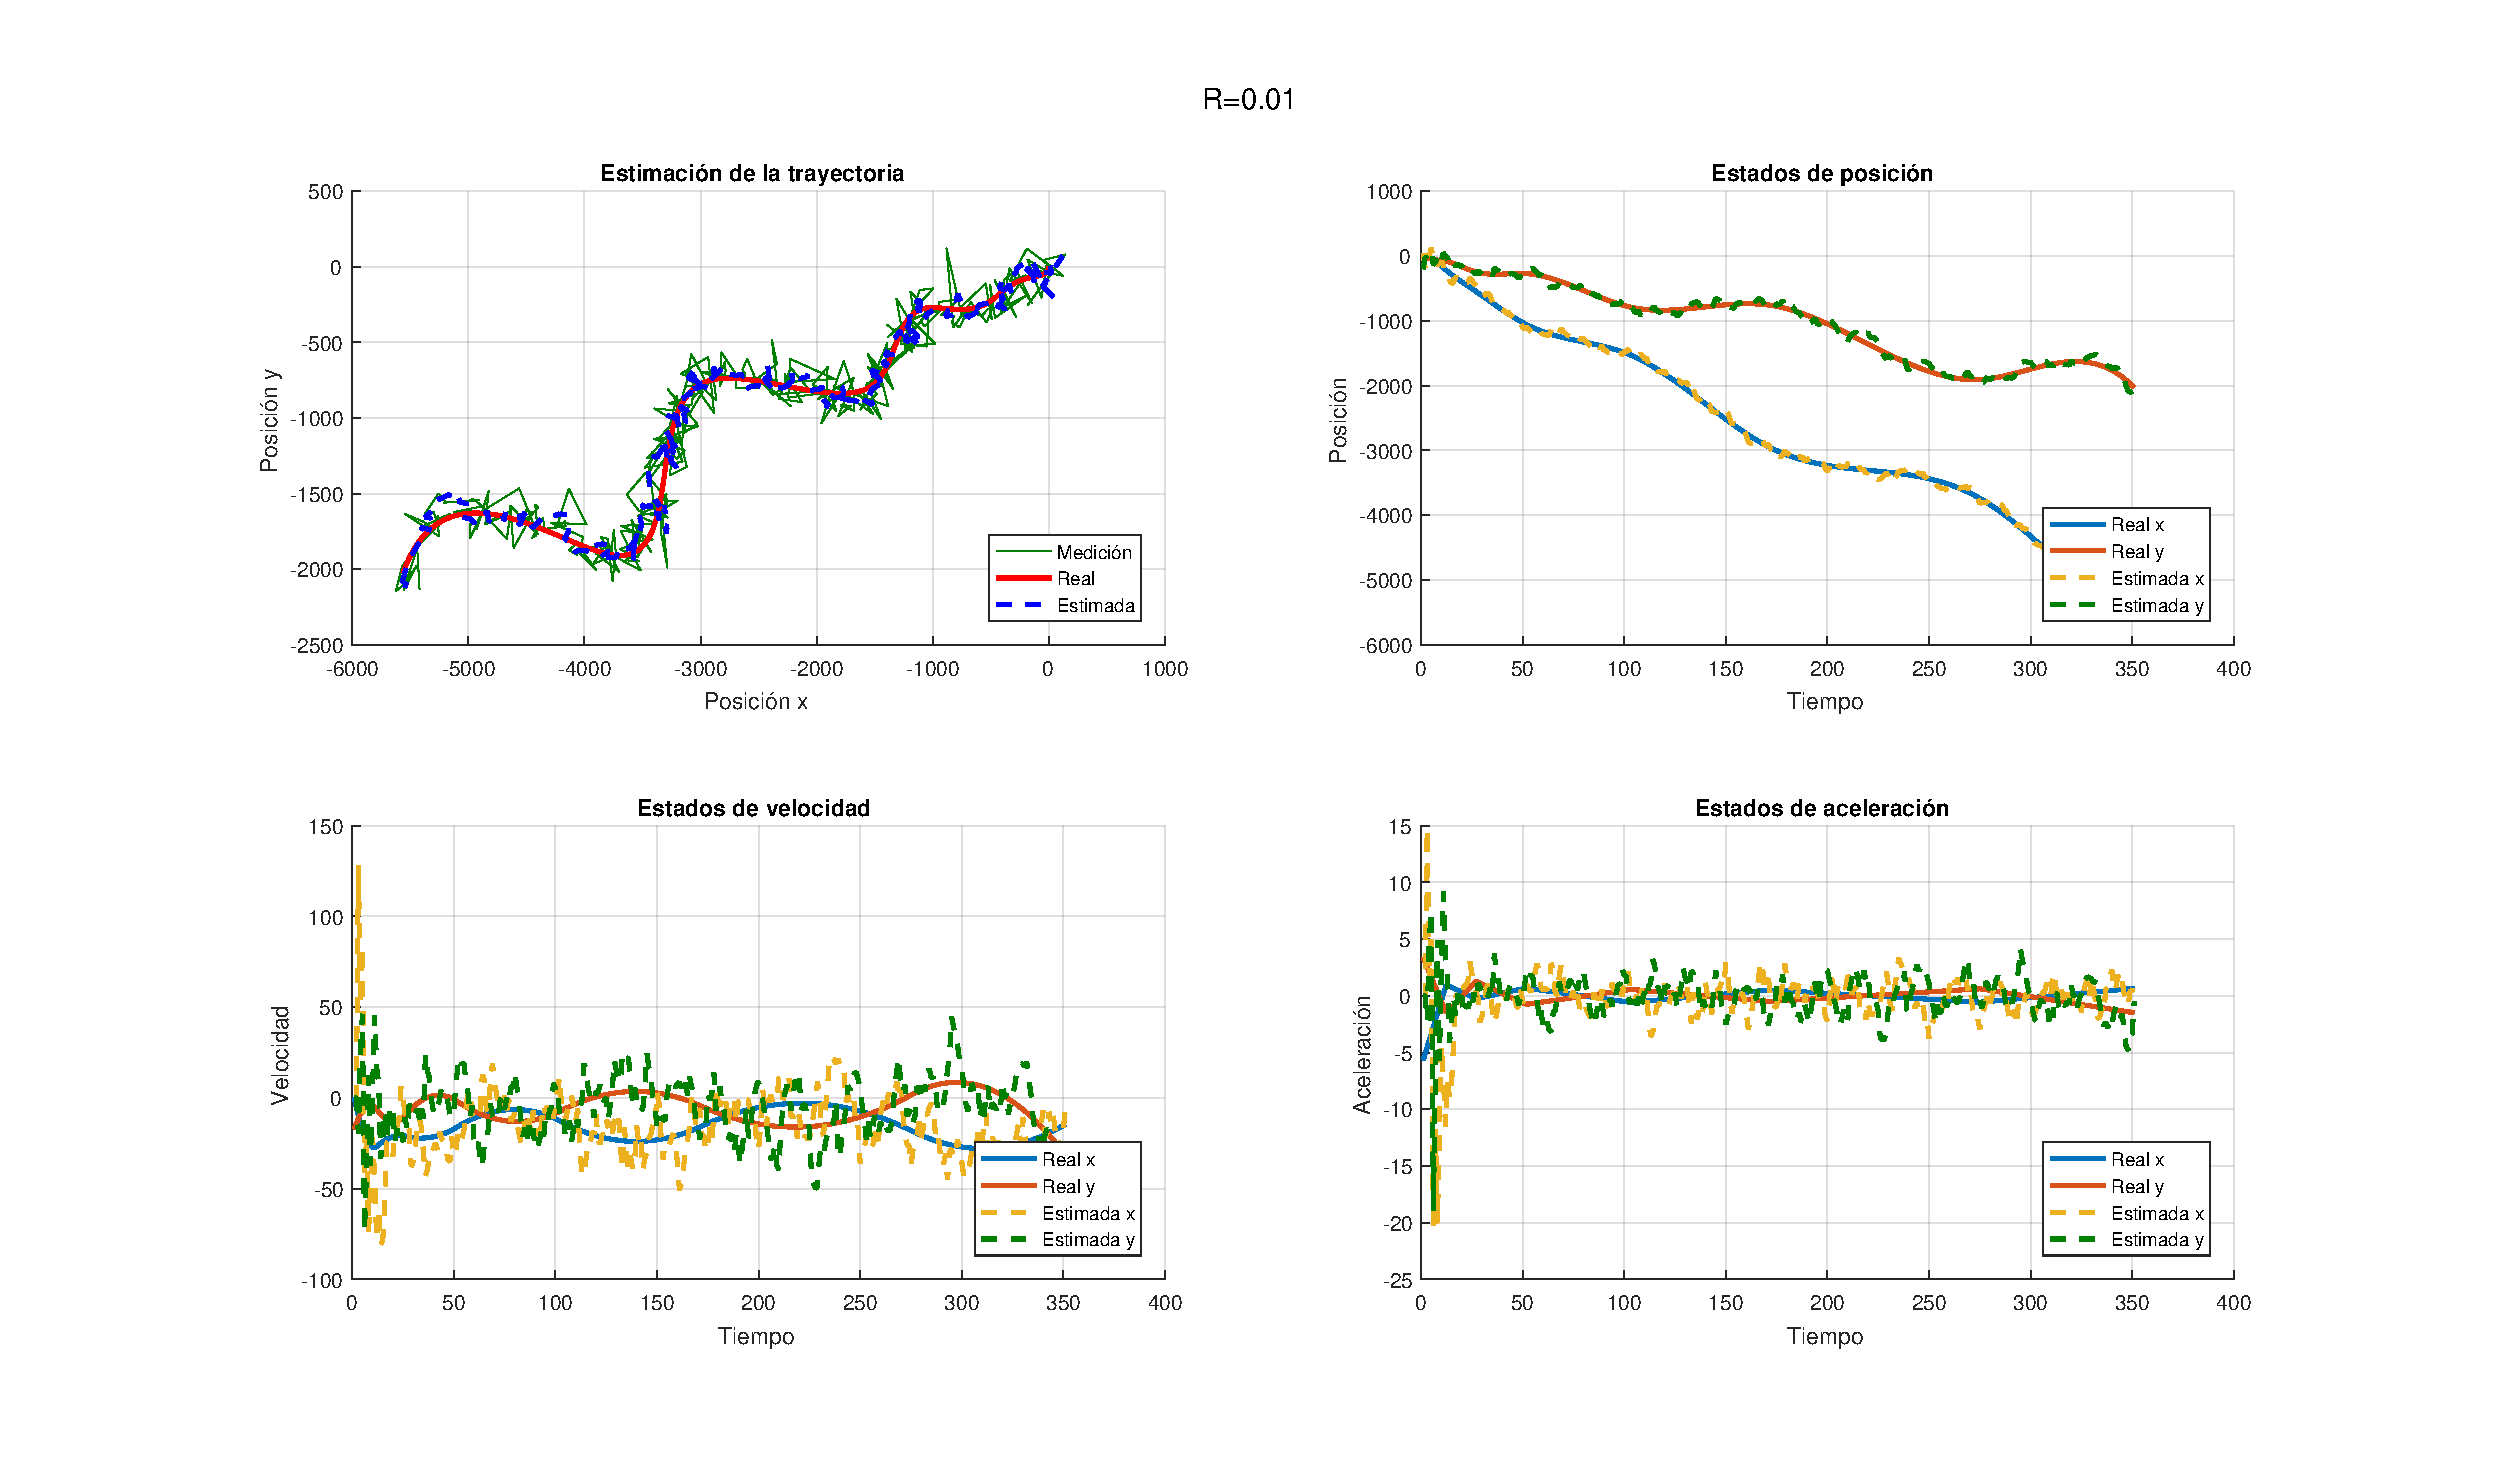
\includegraphics[width=1.0\textwidth,keepaspectratio]{Figuras/graf_ej6_R2.pdf}
		\caption{Estimación de Trayectoria - Matriz de Covarianza Menor}
		\label{fig:ej5r2}
	\end{figure}
	
	En las figuras \ref{fig:ej5r1_innov} y \ref{fig:ej5r2_innov} se observan las autocorrelaciones de las innovaciones. Puede observarse que cuanto mayor sea la matriz de ruido de proceso, el proceso es menos blanco, y por consiguente, se concluye que la estimación es peor.
	
	\begin{figure}[H]
		\centering
		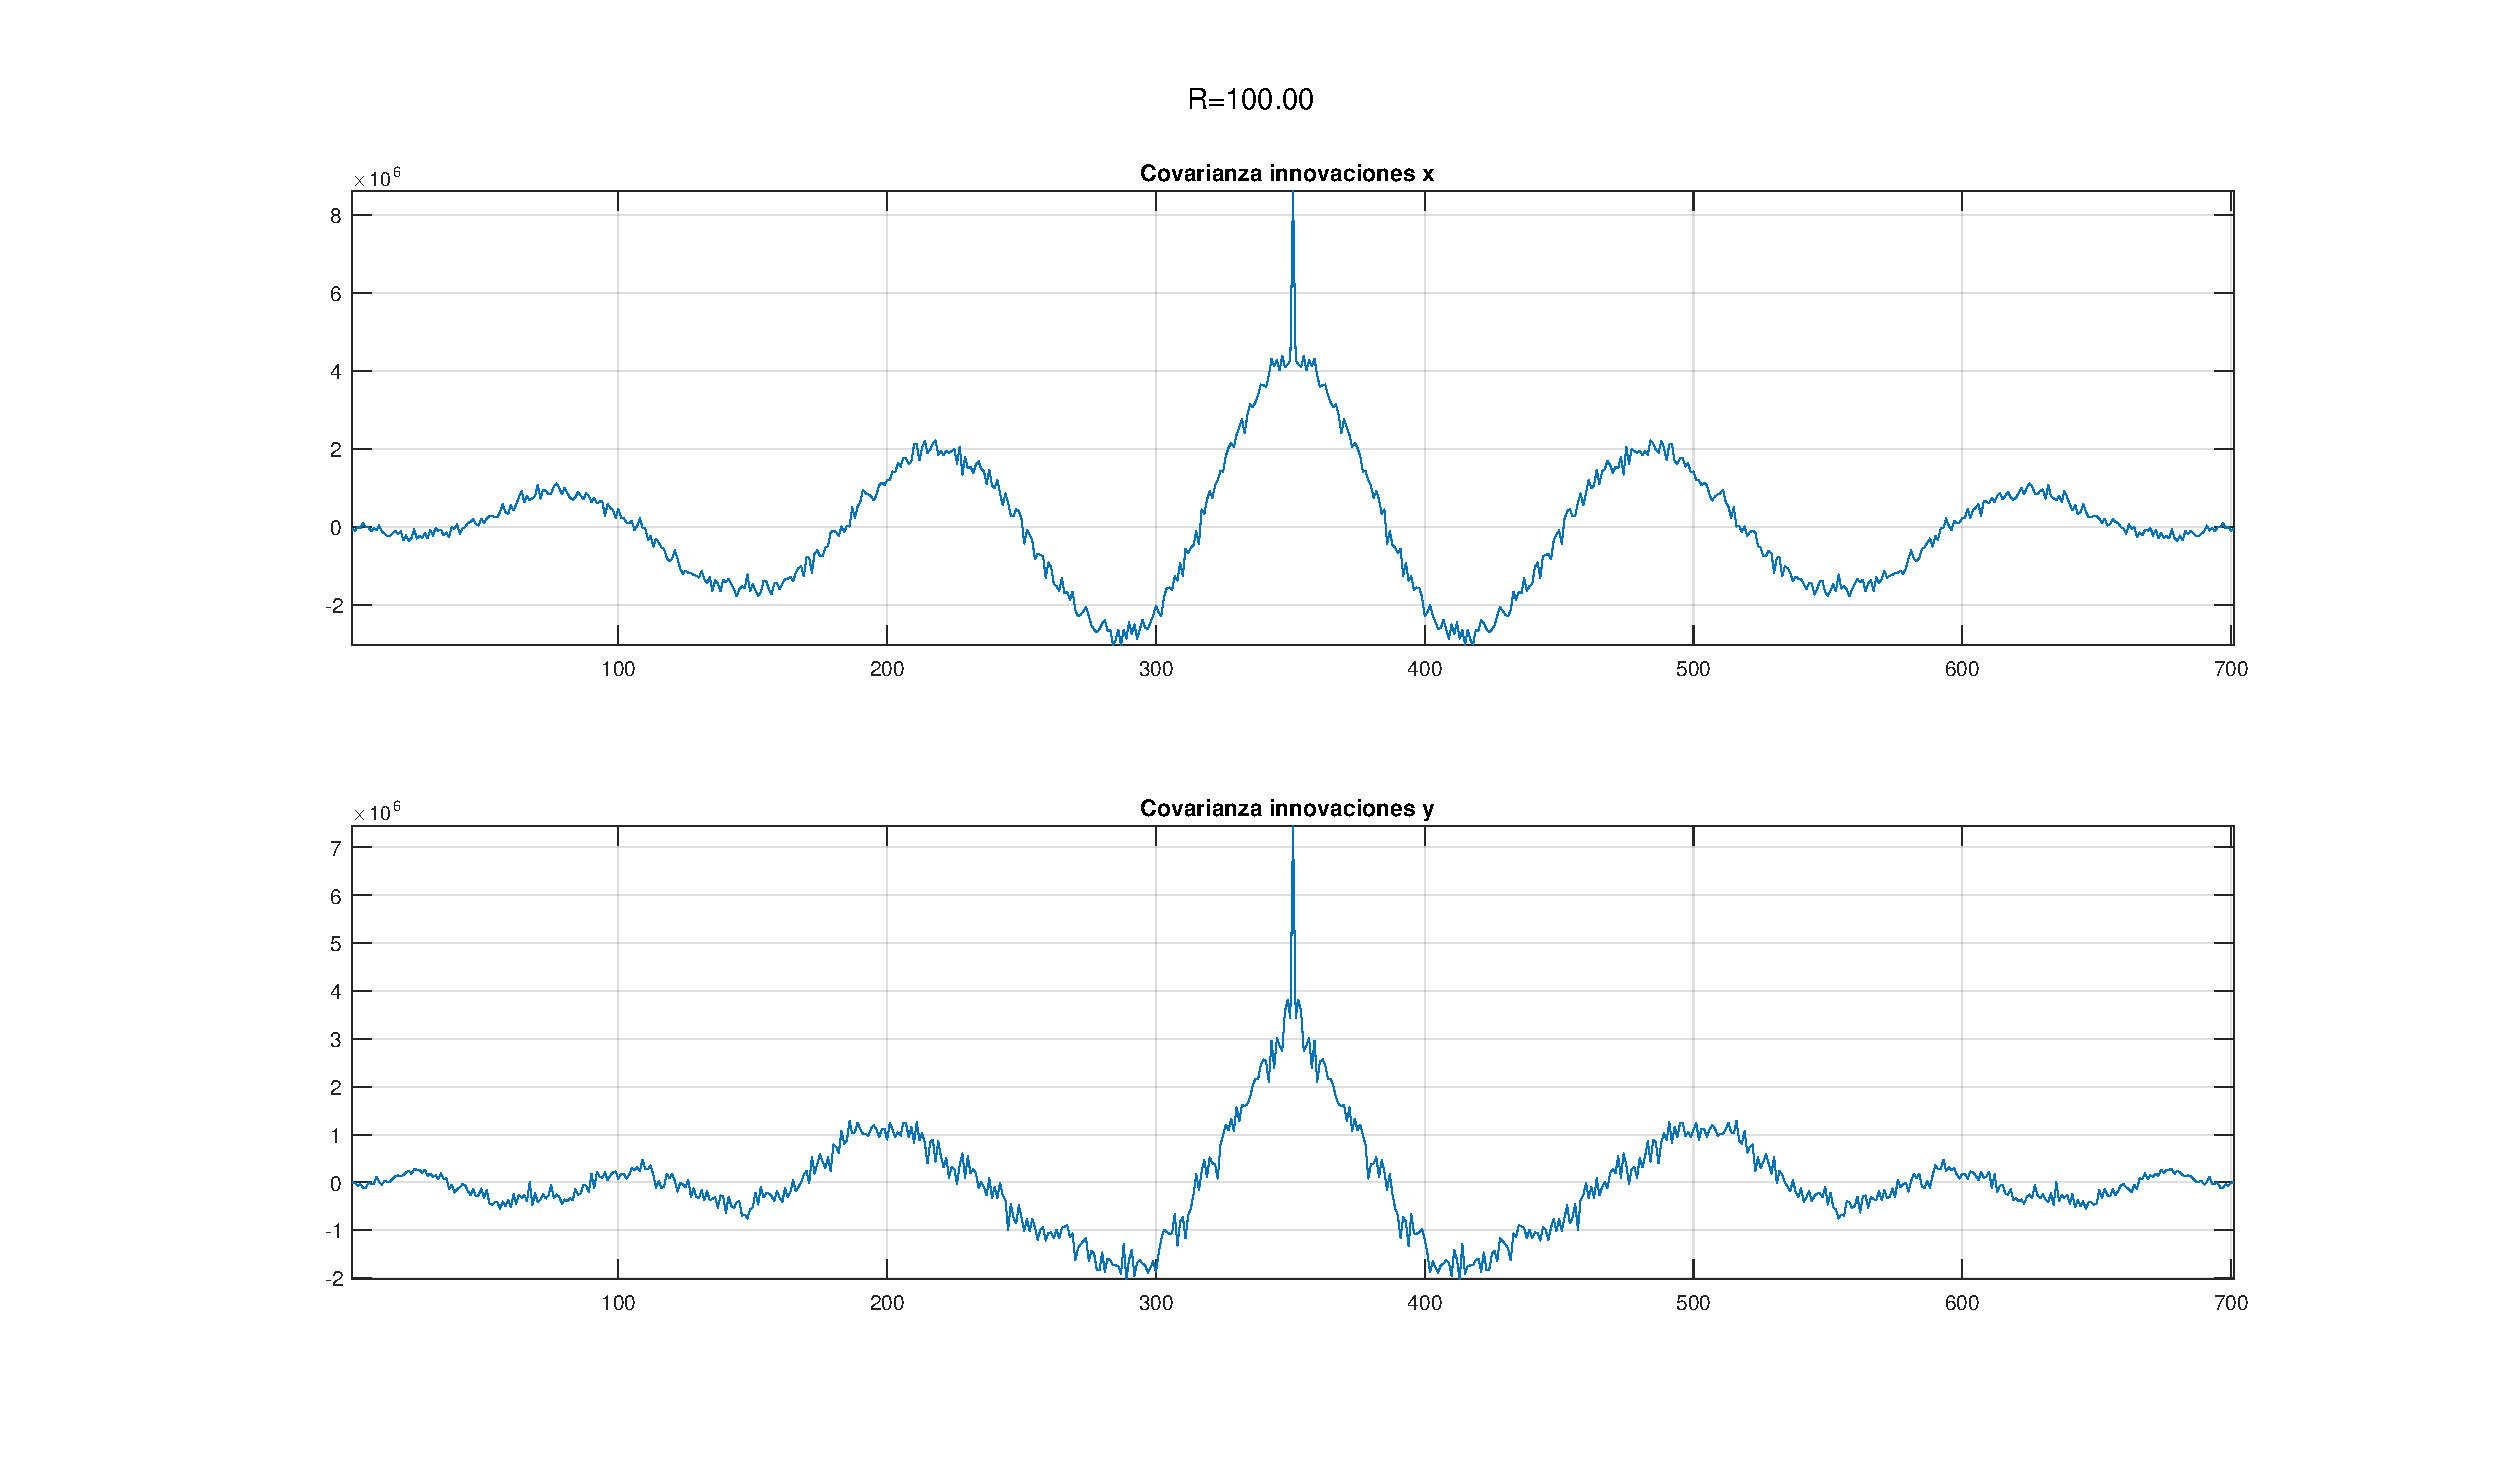
\includegraphics[width=1.0\textwidth,keepaspectratio]{Figuras/covinn_ej6_R1.pdf}
		\caption{Autocorrelación de Innovaciones - Matriz de Covarianza Mayor}
		\label{fig:ej5r1_innov}
	\end{figure}
	
	\begin{figure}[H]
		\centering
		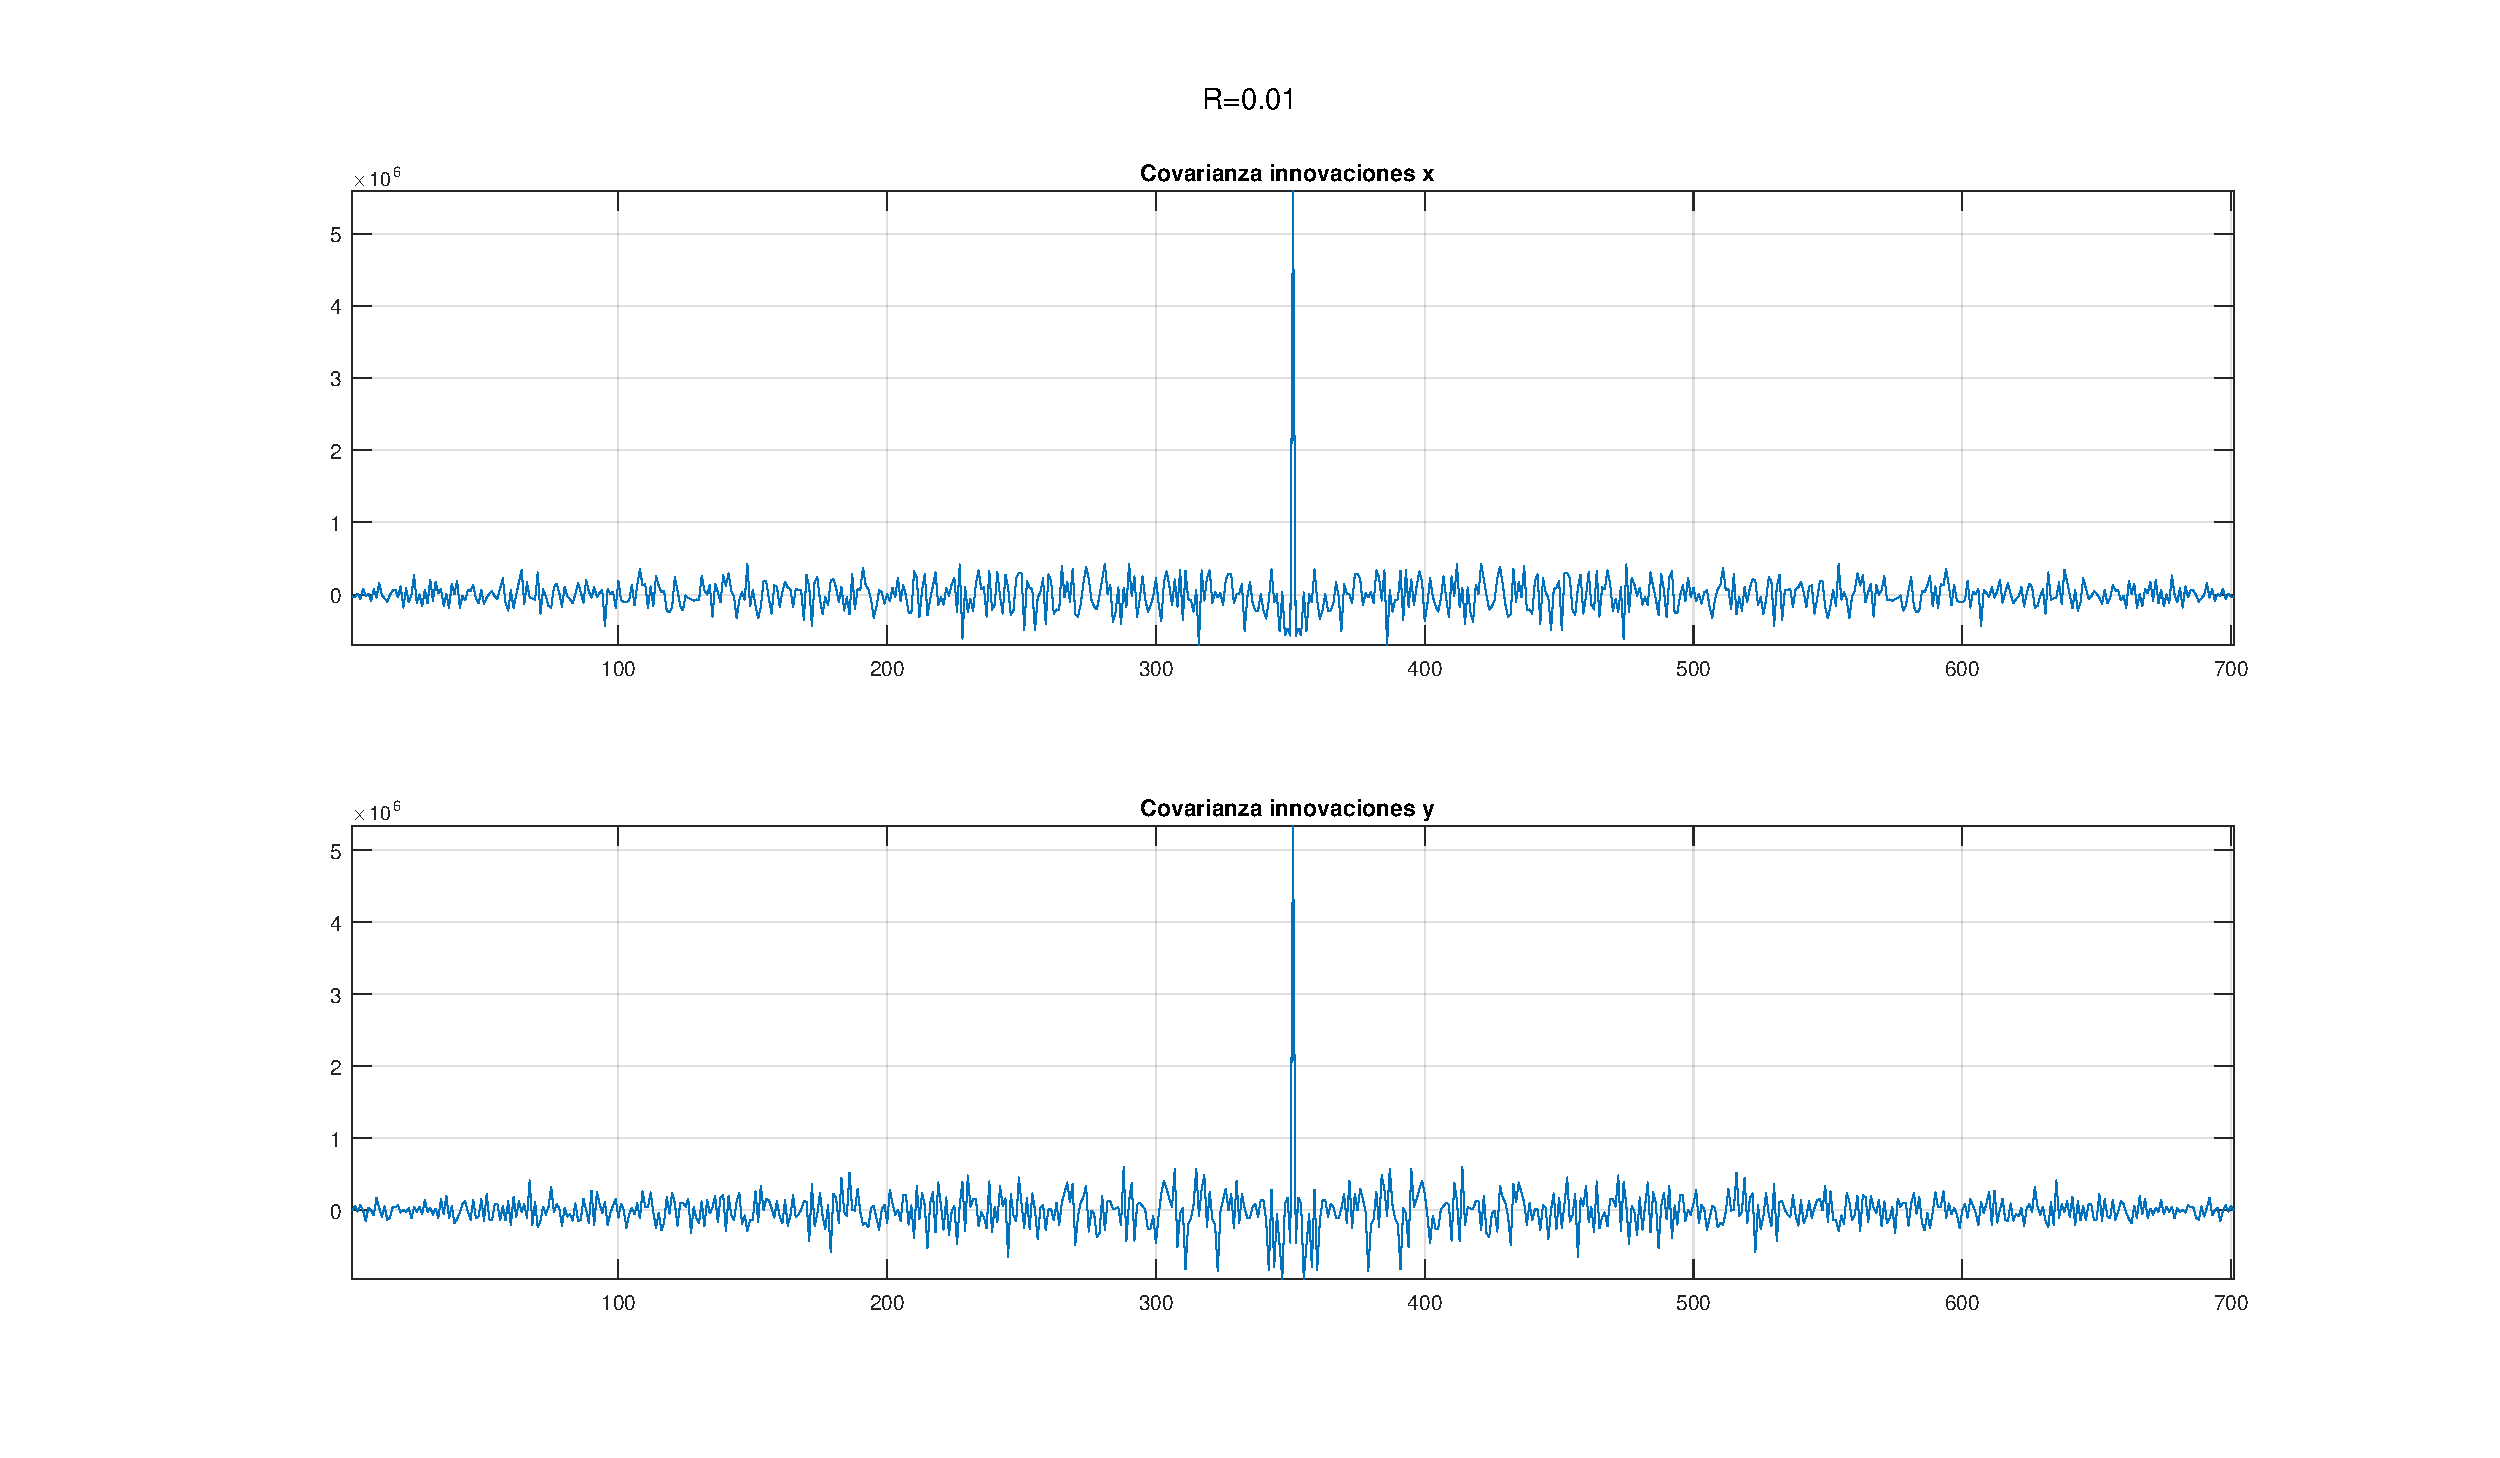
\includegraphics[width=1.0\textwidth,keepaspectratio]{Figuras/covinn_ej6_R2.pdf}
		\caption{Autocorrelación de Innovaciones - Matriz de Covarianza Menor}
		\label{fig:ej5r2_innov}
	\end{figure}
	
%--------------------------------------------------------------------------------------------------

\subsection{Script}

	A continuación incluimos el script que realiza la estimación.
	
	%\lstinputlisting[]{../Octave/EJ6.m}


	\section{Ejercicio 6 \\ Kalman En Estado Estacionario}\label{sec:ej6}
		
	Es importante recalcar, que la ganancia de Kalman $K_k$ es distinta para cada instante $k$. Cuando el sistema es variante en el tiempo, el filtro se adapta a las condiciones de dinámica y ruido instante a instante. Por otro lado cuando el sistema es invariante en el tiempo, puede demostrarse que tanto la matriz $K_k$, como la matriz $P_k$, convergen para tiempo infinito. Es decir:
	
	\begin{equation*}
		K_k \longrightarrow K
	\end{equation*}
	
	\begin{equation*}
		P_k \longrightarrow P
	\end{equation*}
	
	para $k \rightarrow \infty$. Dichas matrices pueden computarse mediante ecuaciones aritméticas discretas de Riccati (DARE). Es decir, $P$ debe cumplir:
	
	\begin{equation*}
		P = A P A^{*} - A P C^{*} (R + C P C^{*})^{-1} C P A + B Q B^{*}
	\end{equation*}
	
	Por otro lado la ganancia de Kalman puede calcularse:
	
	\begin{equation*}
		K = P C^{*} (R + C P C^{*})^{-1}
	\end{equation*}
	
	Dadas estas matrices, surge la posibilidad de implementar una modificación al algoritmo de Kalman, para que en lugar de utilizar las matrices calculadas instante a instante, siempre utilice las matrices a las que va a converger, suponiendo por supuesto que el sistema es invariante en el tiempo. Dicho algoritmo tiene la ventaja de que posee menos procesamiento en tiempo real, dado a que las matrices $K$ y $P$ pueden computarse en tiempo de compilación y guardarse fijas en la memoria. Dicho algoritmo no será óptimo, pero puede demostrarse que la versión modificada convergerá a la versión original con rapidez exponencial, siendo más los beneficios que trae, que los inconvenientes. El objetivo de este punto es comparar las dos variantes y demostrar esto. En la figura \ref{fig:ej3f_cov} podemos ver el resultado de la estimación. En linea punteada azul puede verse la estimación del algoritmo modificado. Puede verse que comienza desviado de la trayectoria, pero rapidamente converge a la misma. 

	\begin{figure}[H]
		\centering
		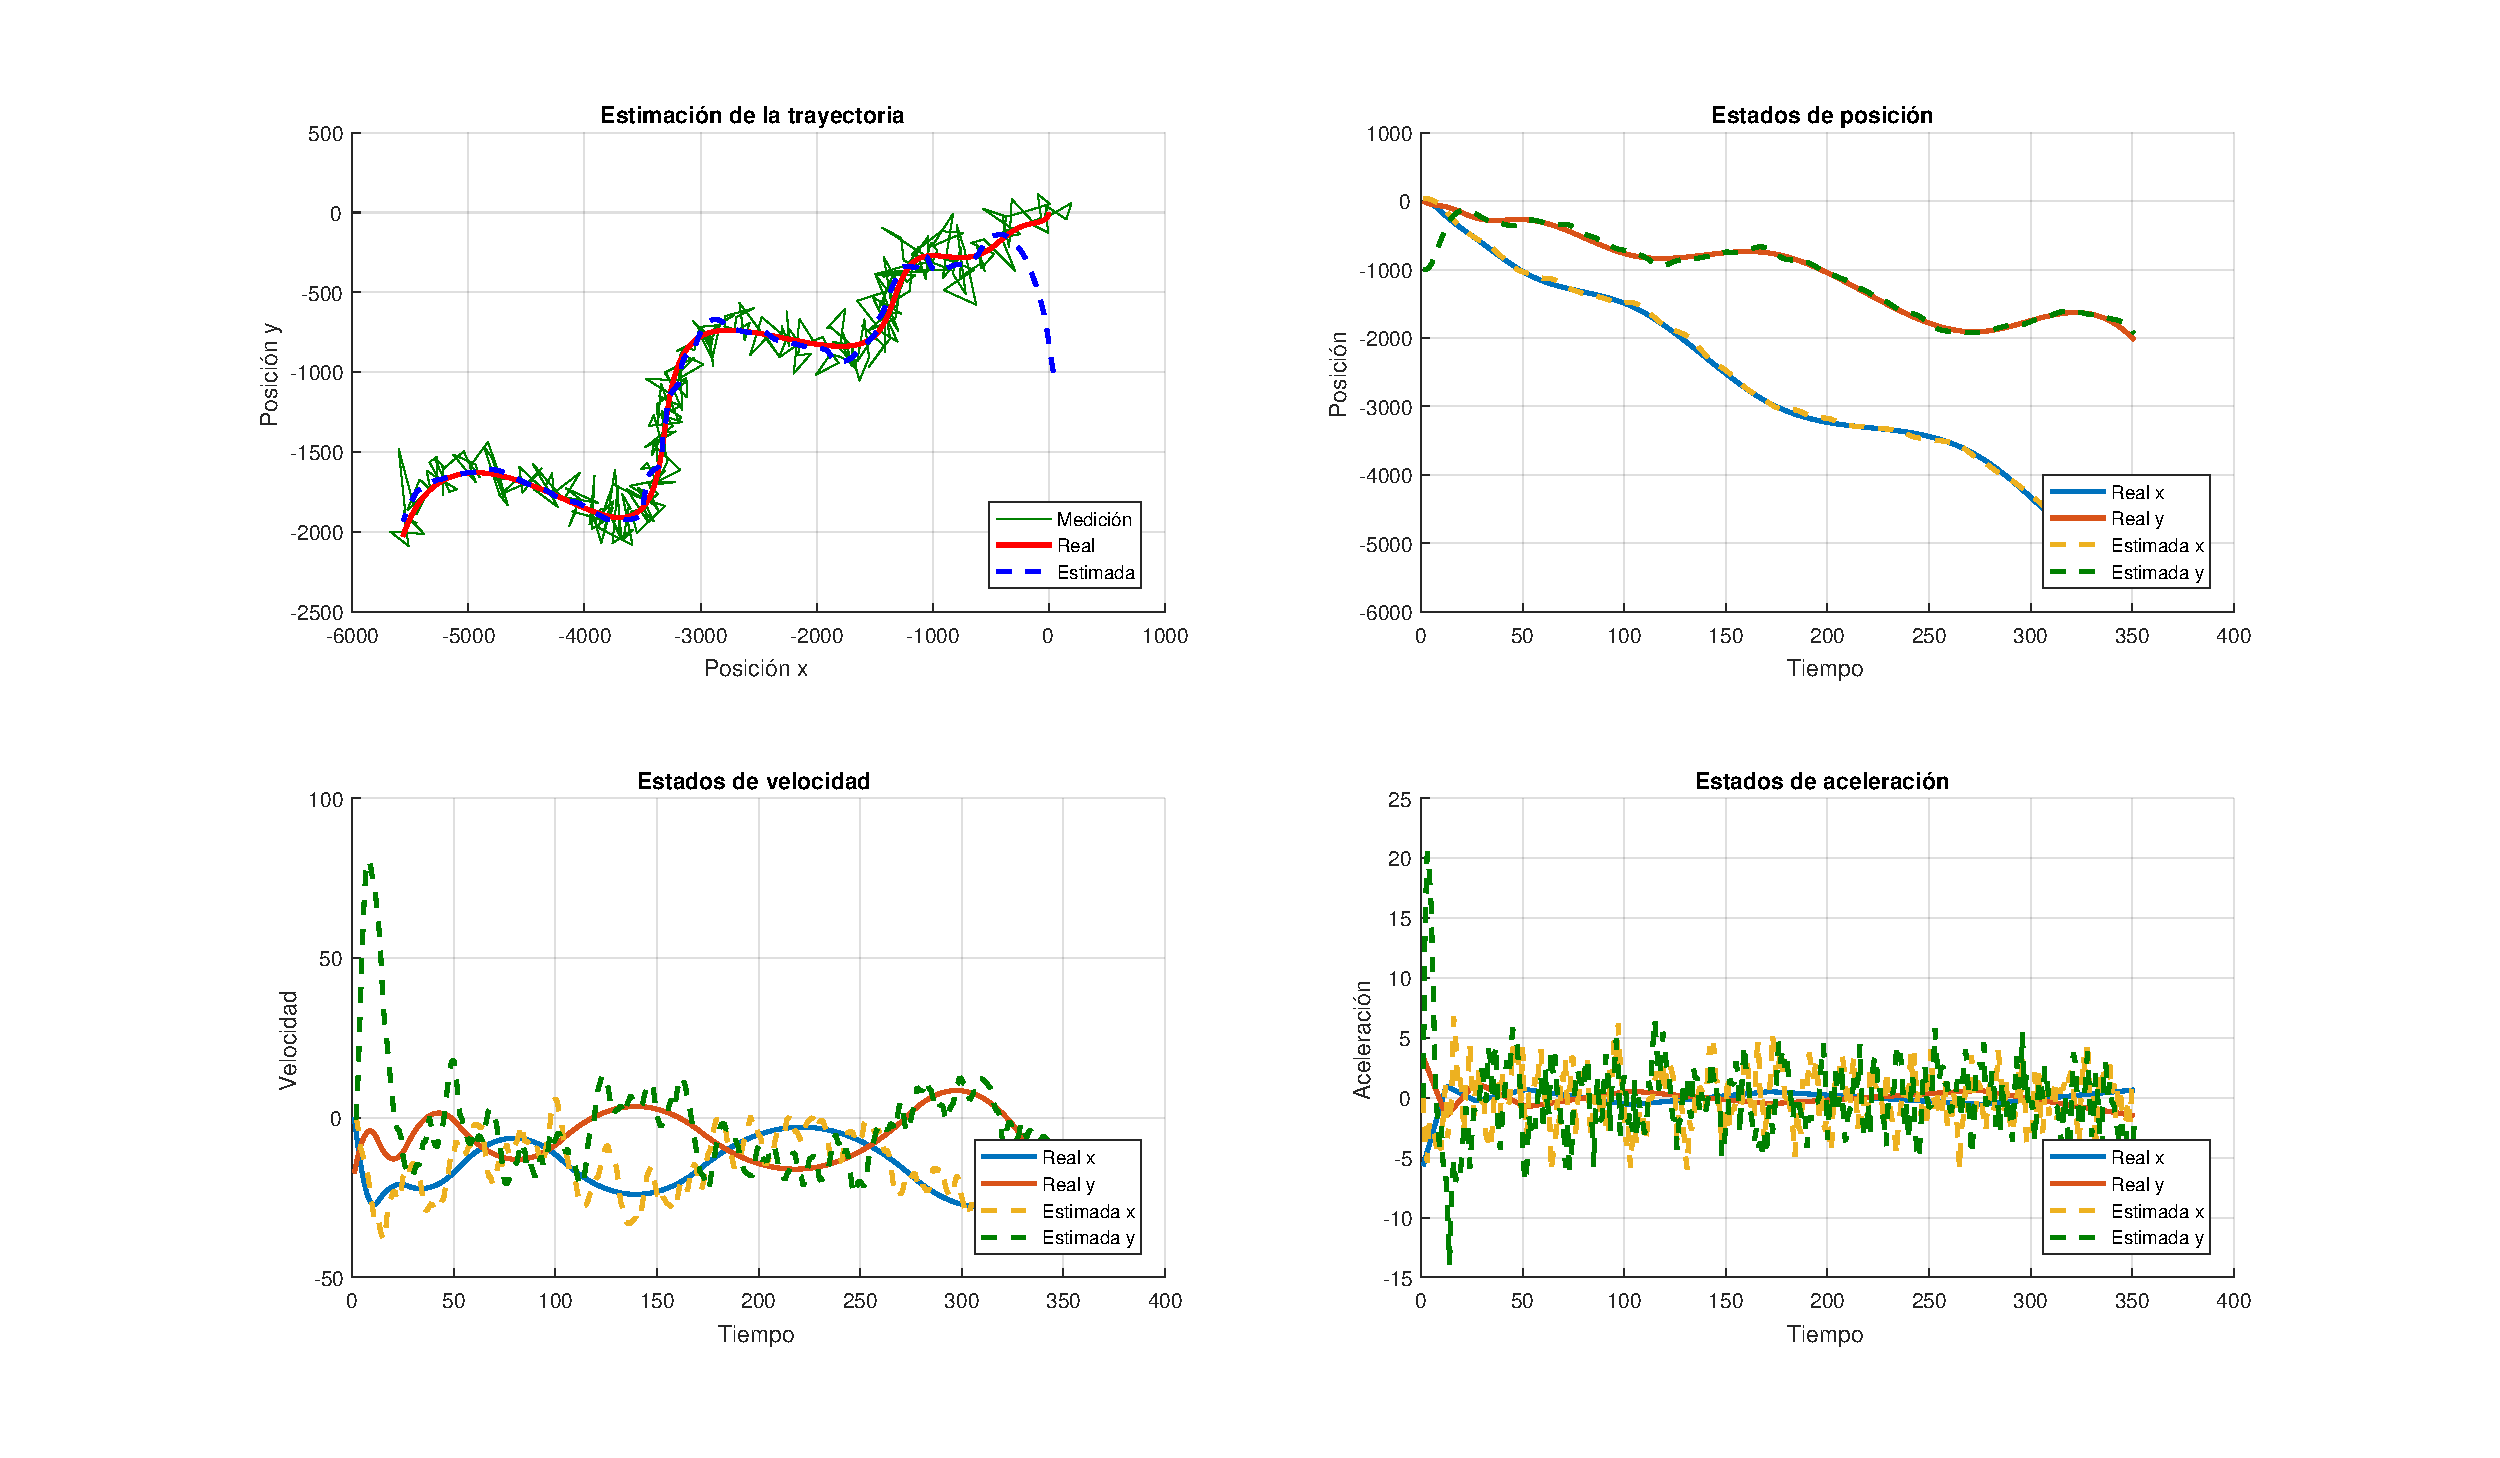
\includegraphics[width=1.0\textwidth,keepaspectratio]{Figuras/graf_ej5.pdf}
		\caption{Estimación de Trayectoria}
		\label{fig:ej6_cov}
	\end{figure}
	
	%Esta otra figura no se a que corresponde.
	%\begin{figure}[H]
	%	\centering
	%	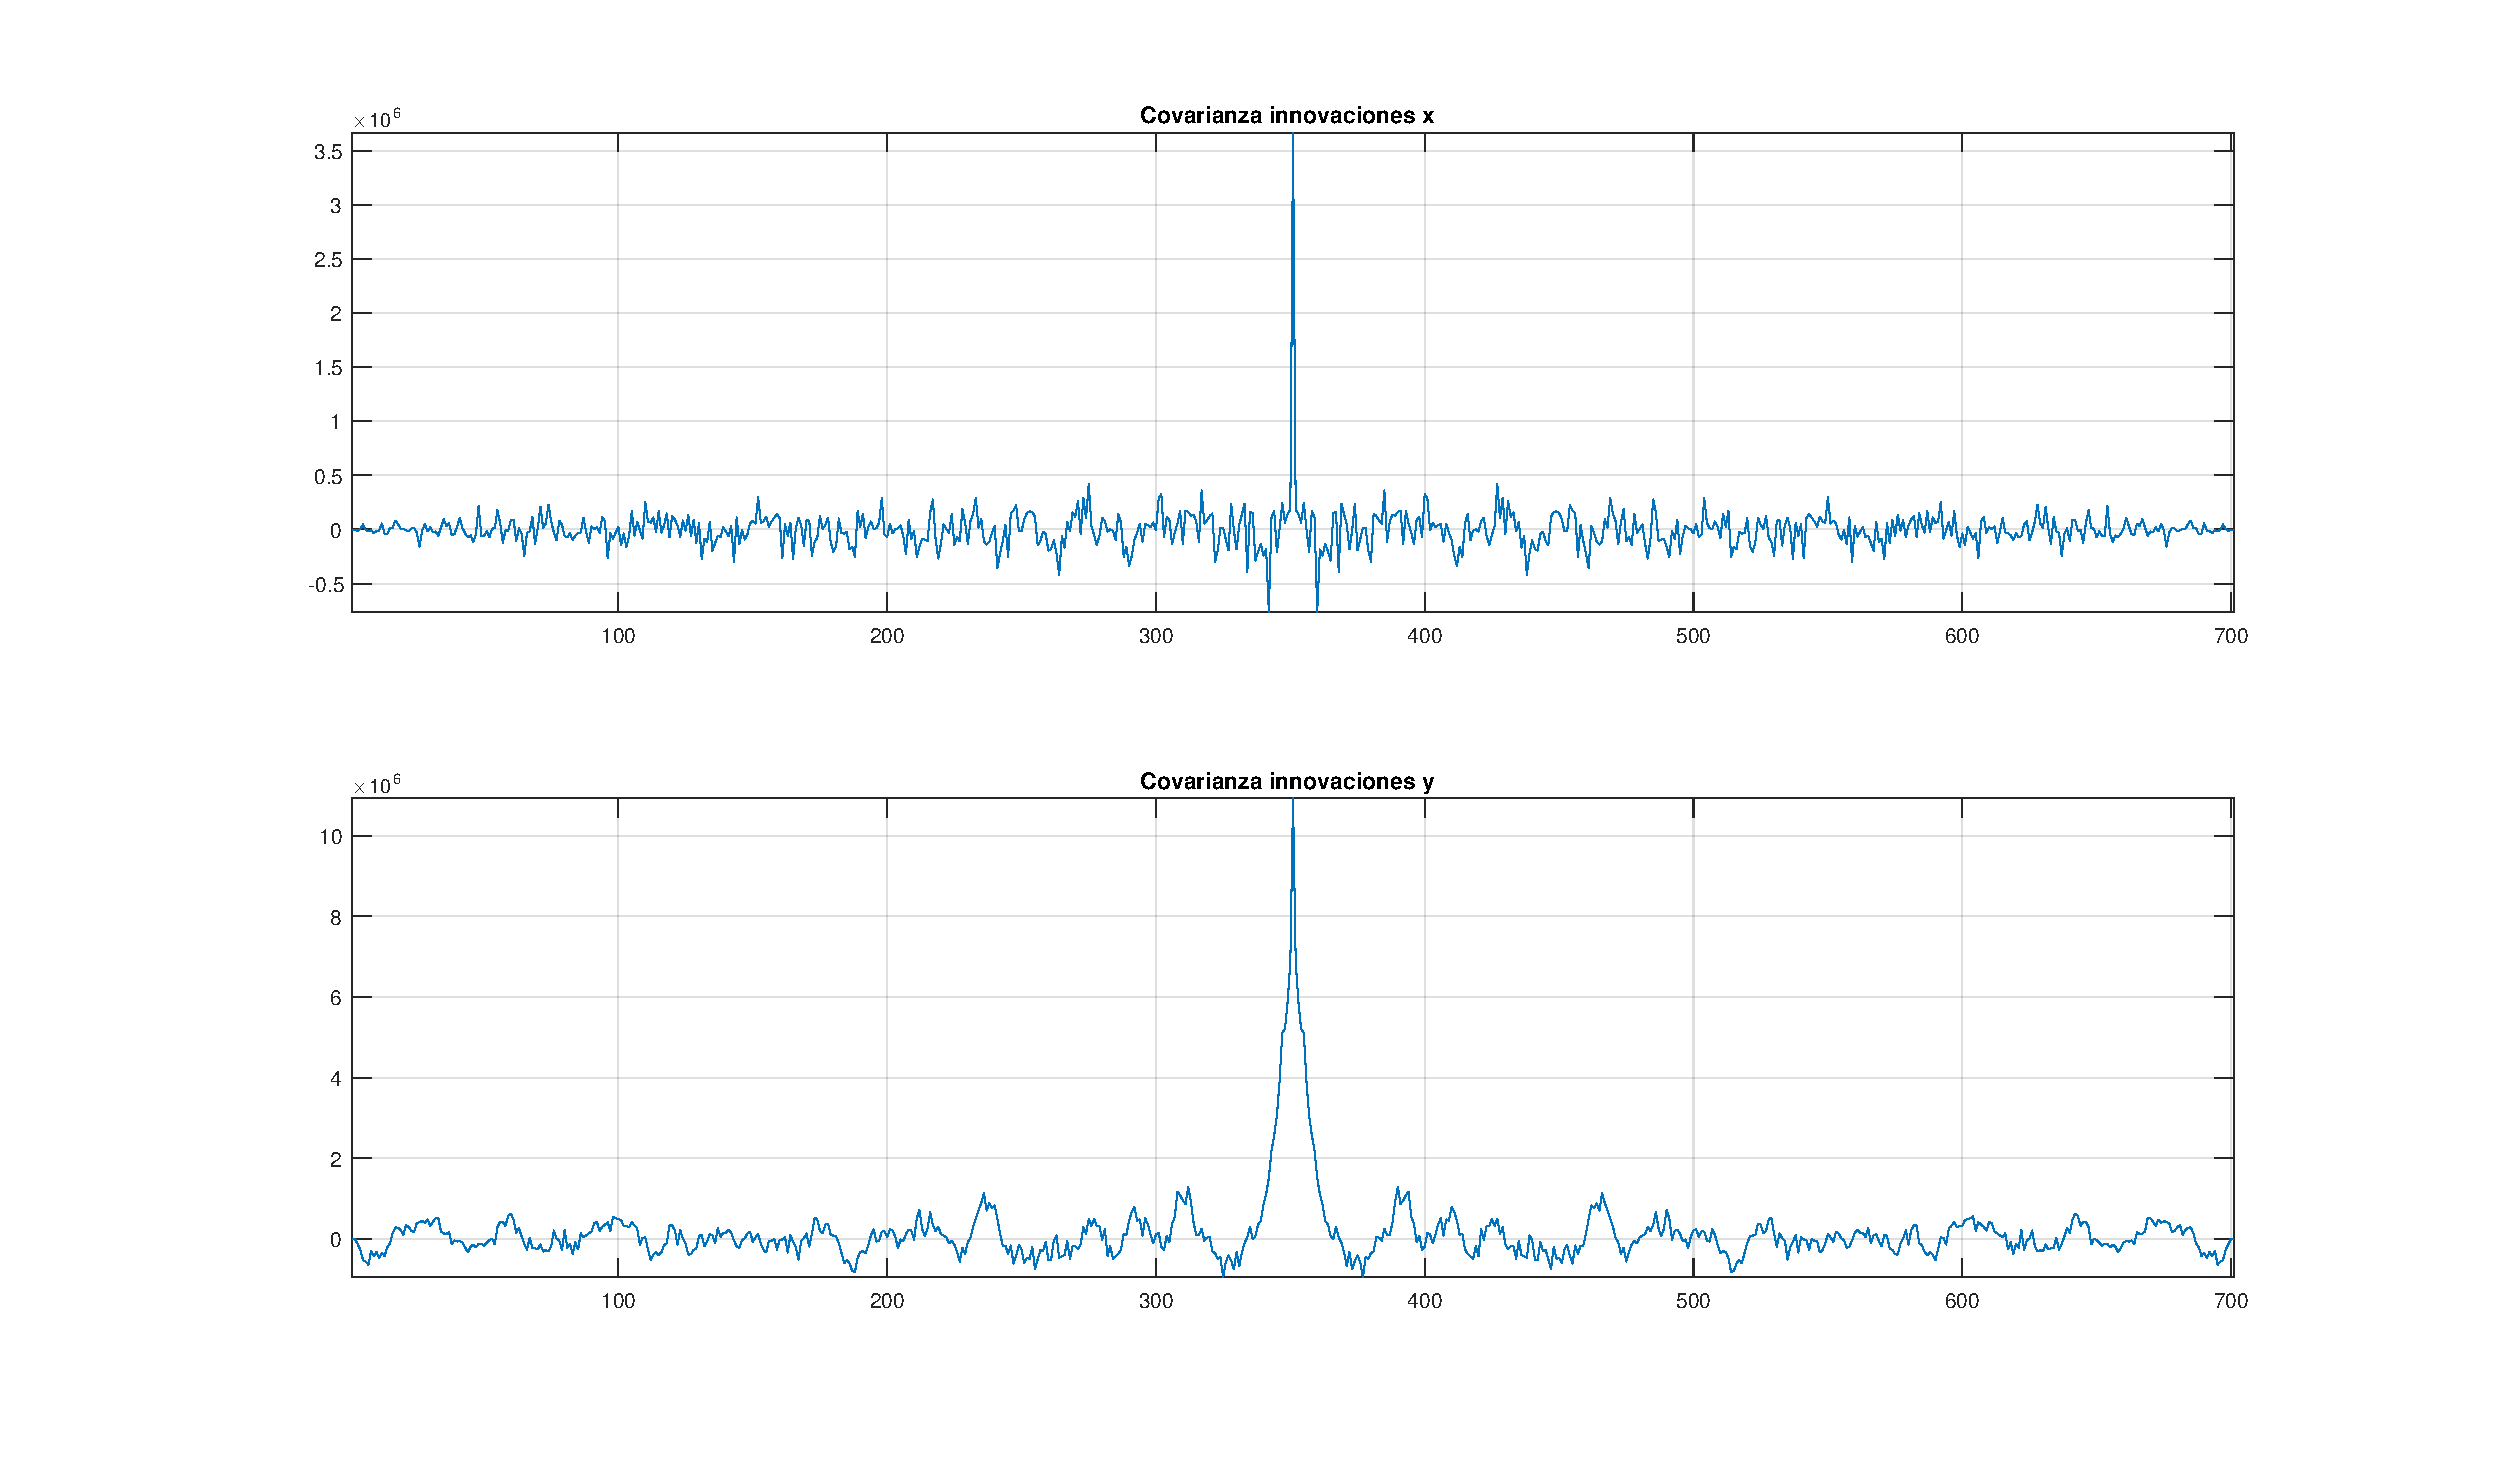
\includegraphics[width=1.0\textwidth,keepaspectratio]{Figuras/covinn_ej5.pdf}
	%	\caption{Correlación De Innovaciones}
	%	\label{fig:ej6_cov}
	%\end{figure}
	
	\subsection{Script}

	A continuación incluimos el script que realiza la estimación.
	
	%\lstinputlisting[]{../Octave/EJ5.m}


	\section{Ejercicio 7 \\ Perdida De Datos}\label{sec:ej7}
		
	Si bien hasta ahora en la simulación se han utilizado datos de las mediciones en forma equiespaciada, en las aplicaciones prácticas muchas veces no se sabe en qué momento se recibirá la próxima medición, o incluso puede darse que se reciba información de distintos sensores con distinta frecuencia. El objetivo de este punto es ver cómo se comporta el filtro de Kalman ante la falta o pérdida de datos en algunos instantes. Para poder simular ésto se dispone de dos mecanismos distintos: el primer método para simularlo es utilizando una matriz de salida $C_d$ dinámica que se modifique en función de los datos de los sensores disponibles en un determinado instante. La segunda variante es utilizar una matriz $C_d$ de tamaño fijo, e insertar ceros en lugar de las matrices de identidad por cada vez que se pierde un dato o no se dispone de una medición de ese sensor. Dado que disponer de memoria dinámica para la matriz $C_d$ es un poco mas costoso en los sistemas reales, se ha optado por la segunda alternativa.
	
	\subsection{10\% de pérdida}
	
	\begin{figure}[H]
		\centering
		%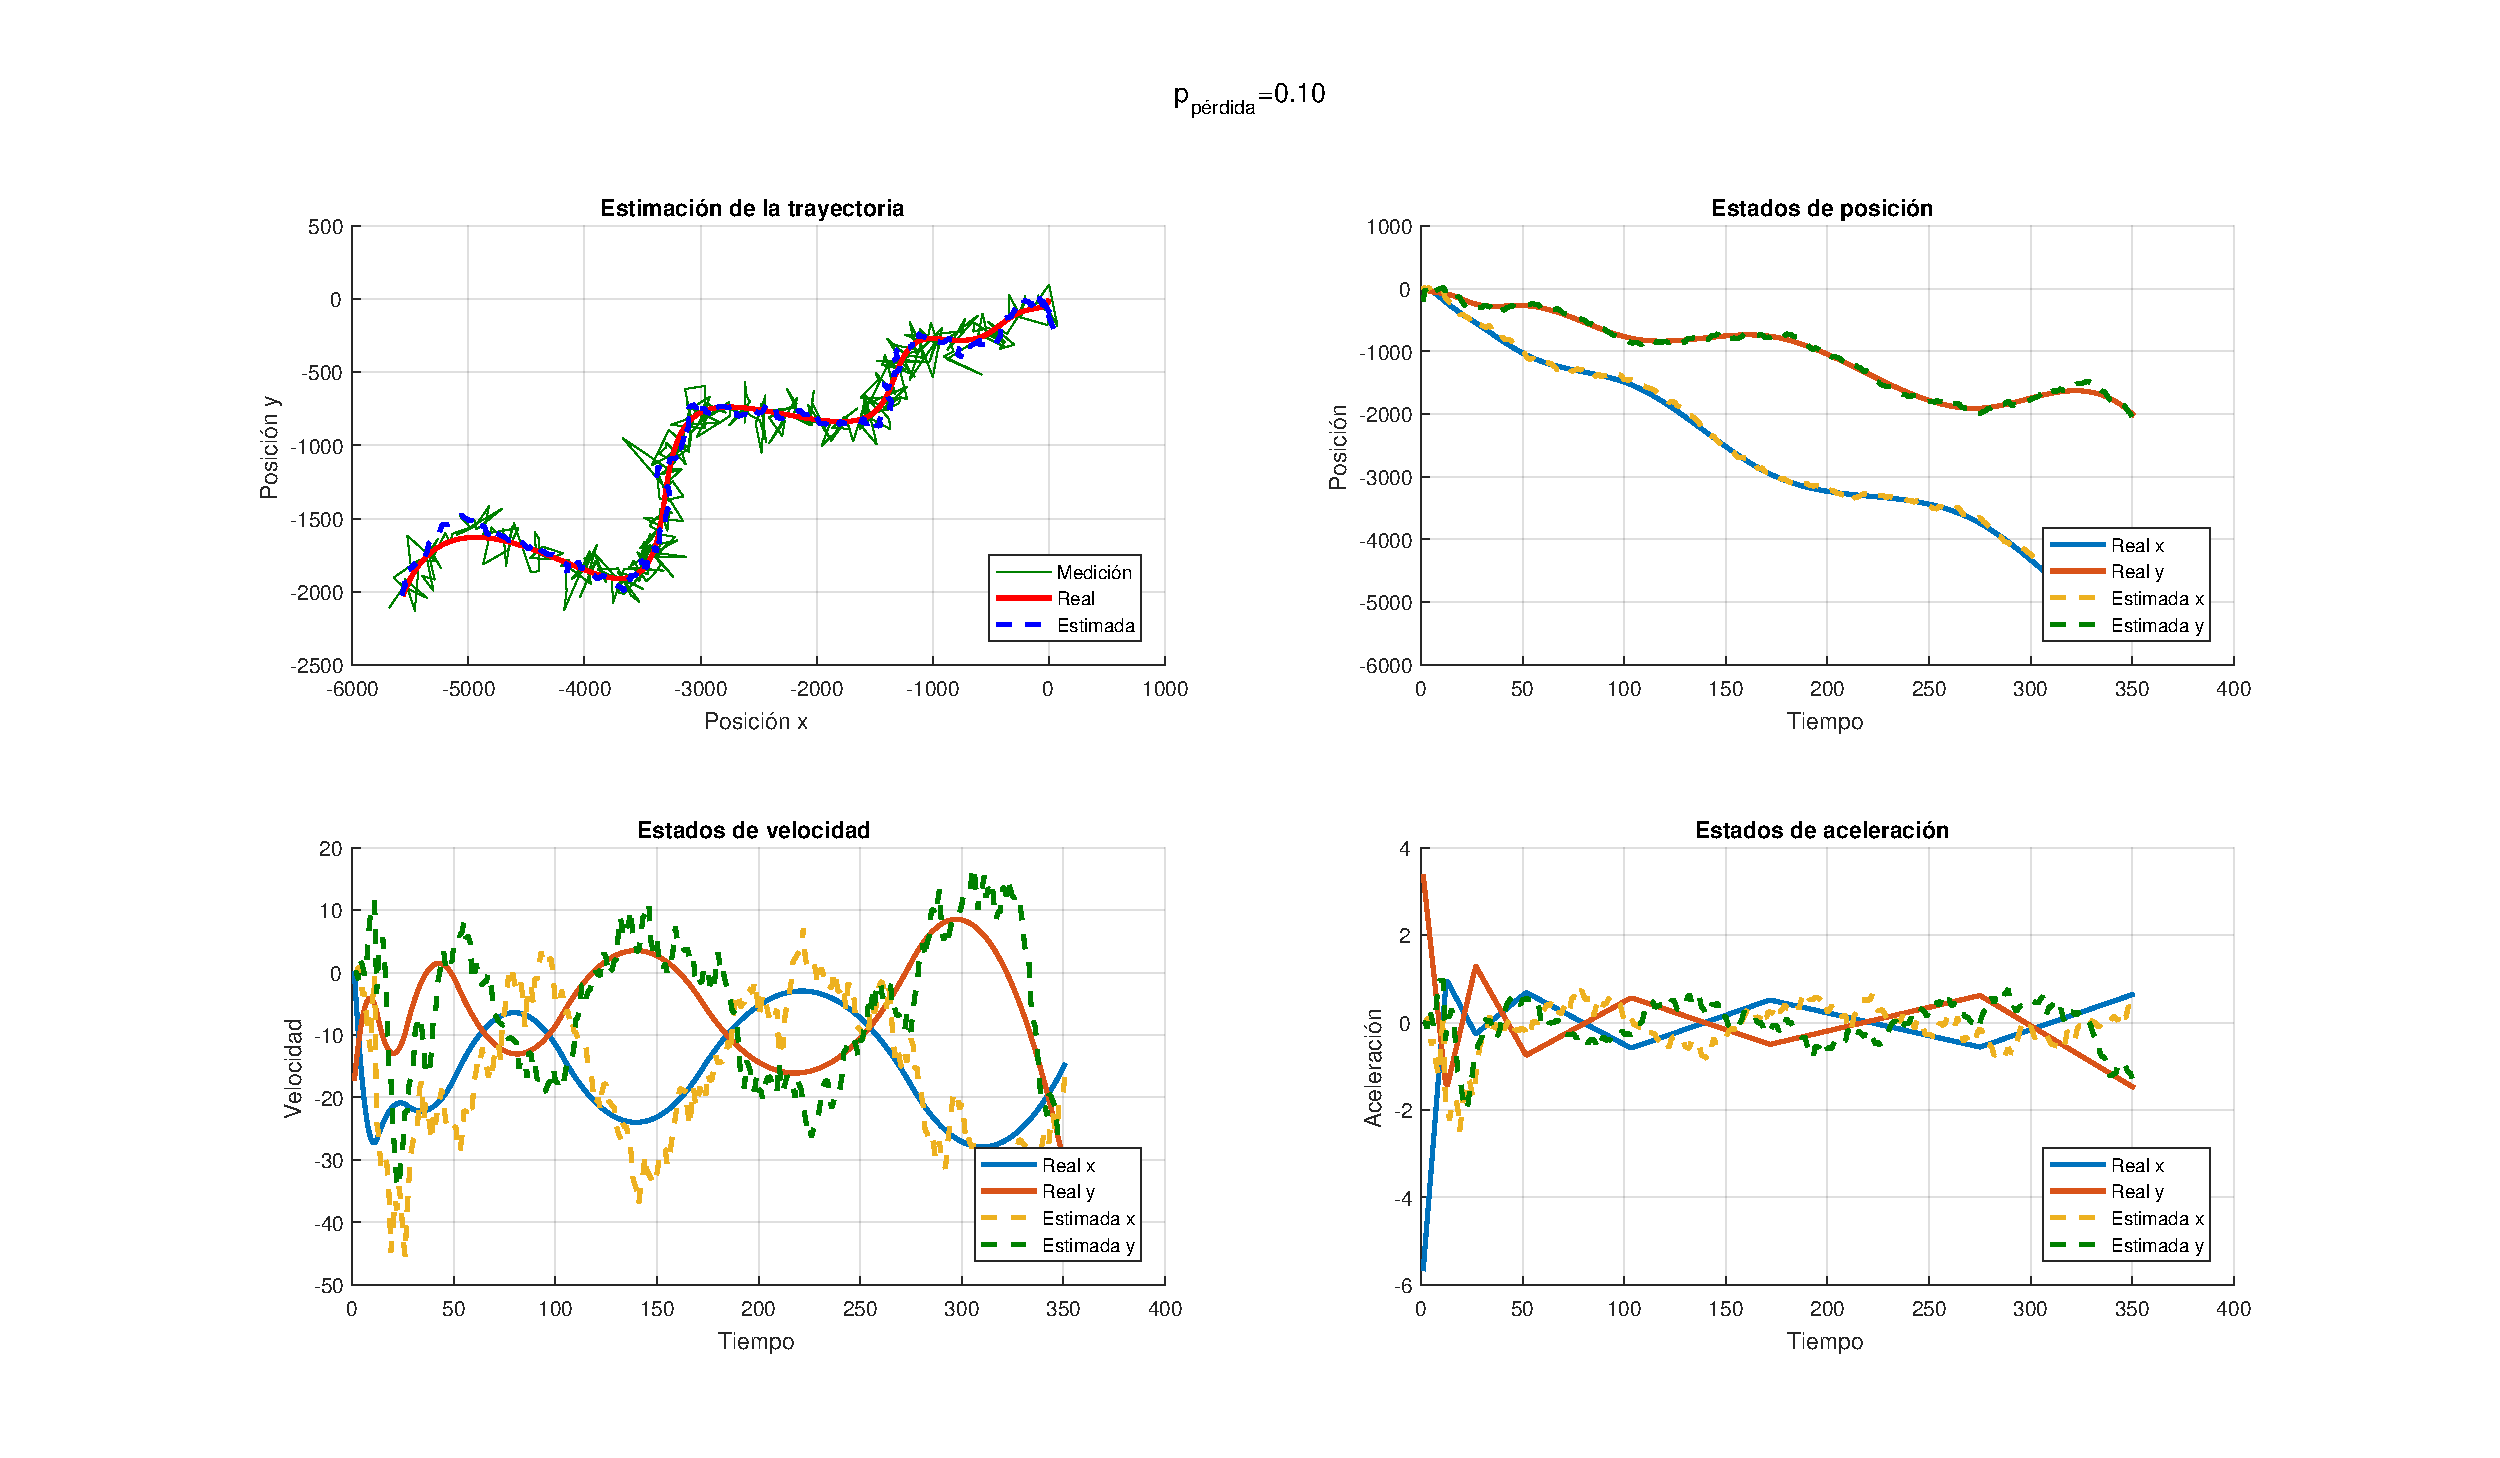
\includegraphics[width=1.0\textwidth,keepaspectratio]{Figuras/graf_ej7_1.pdf}
		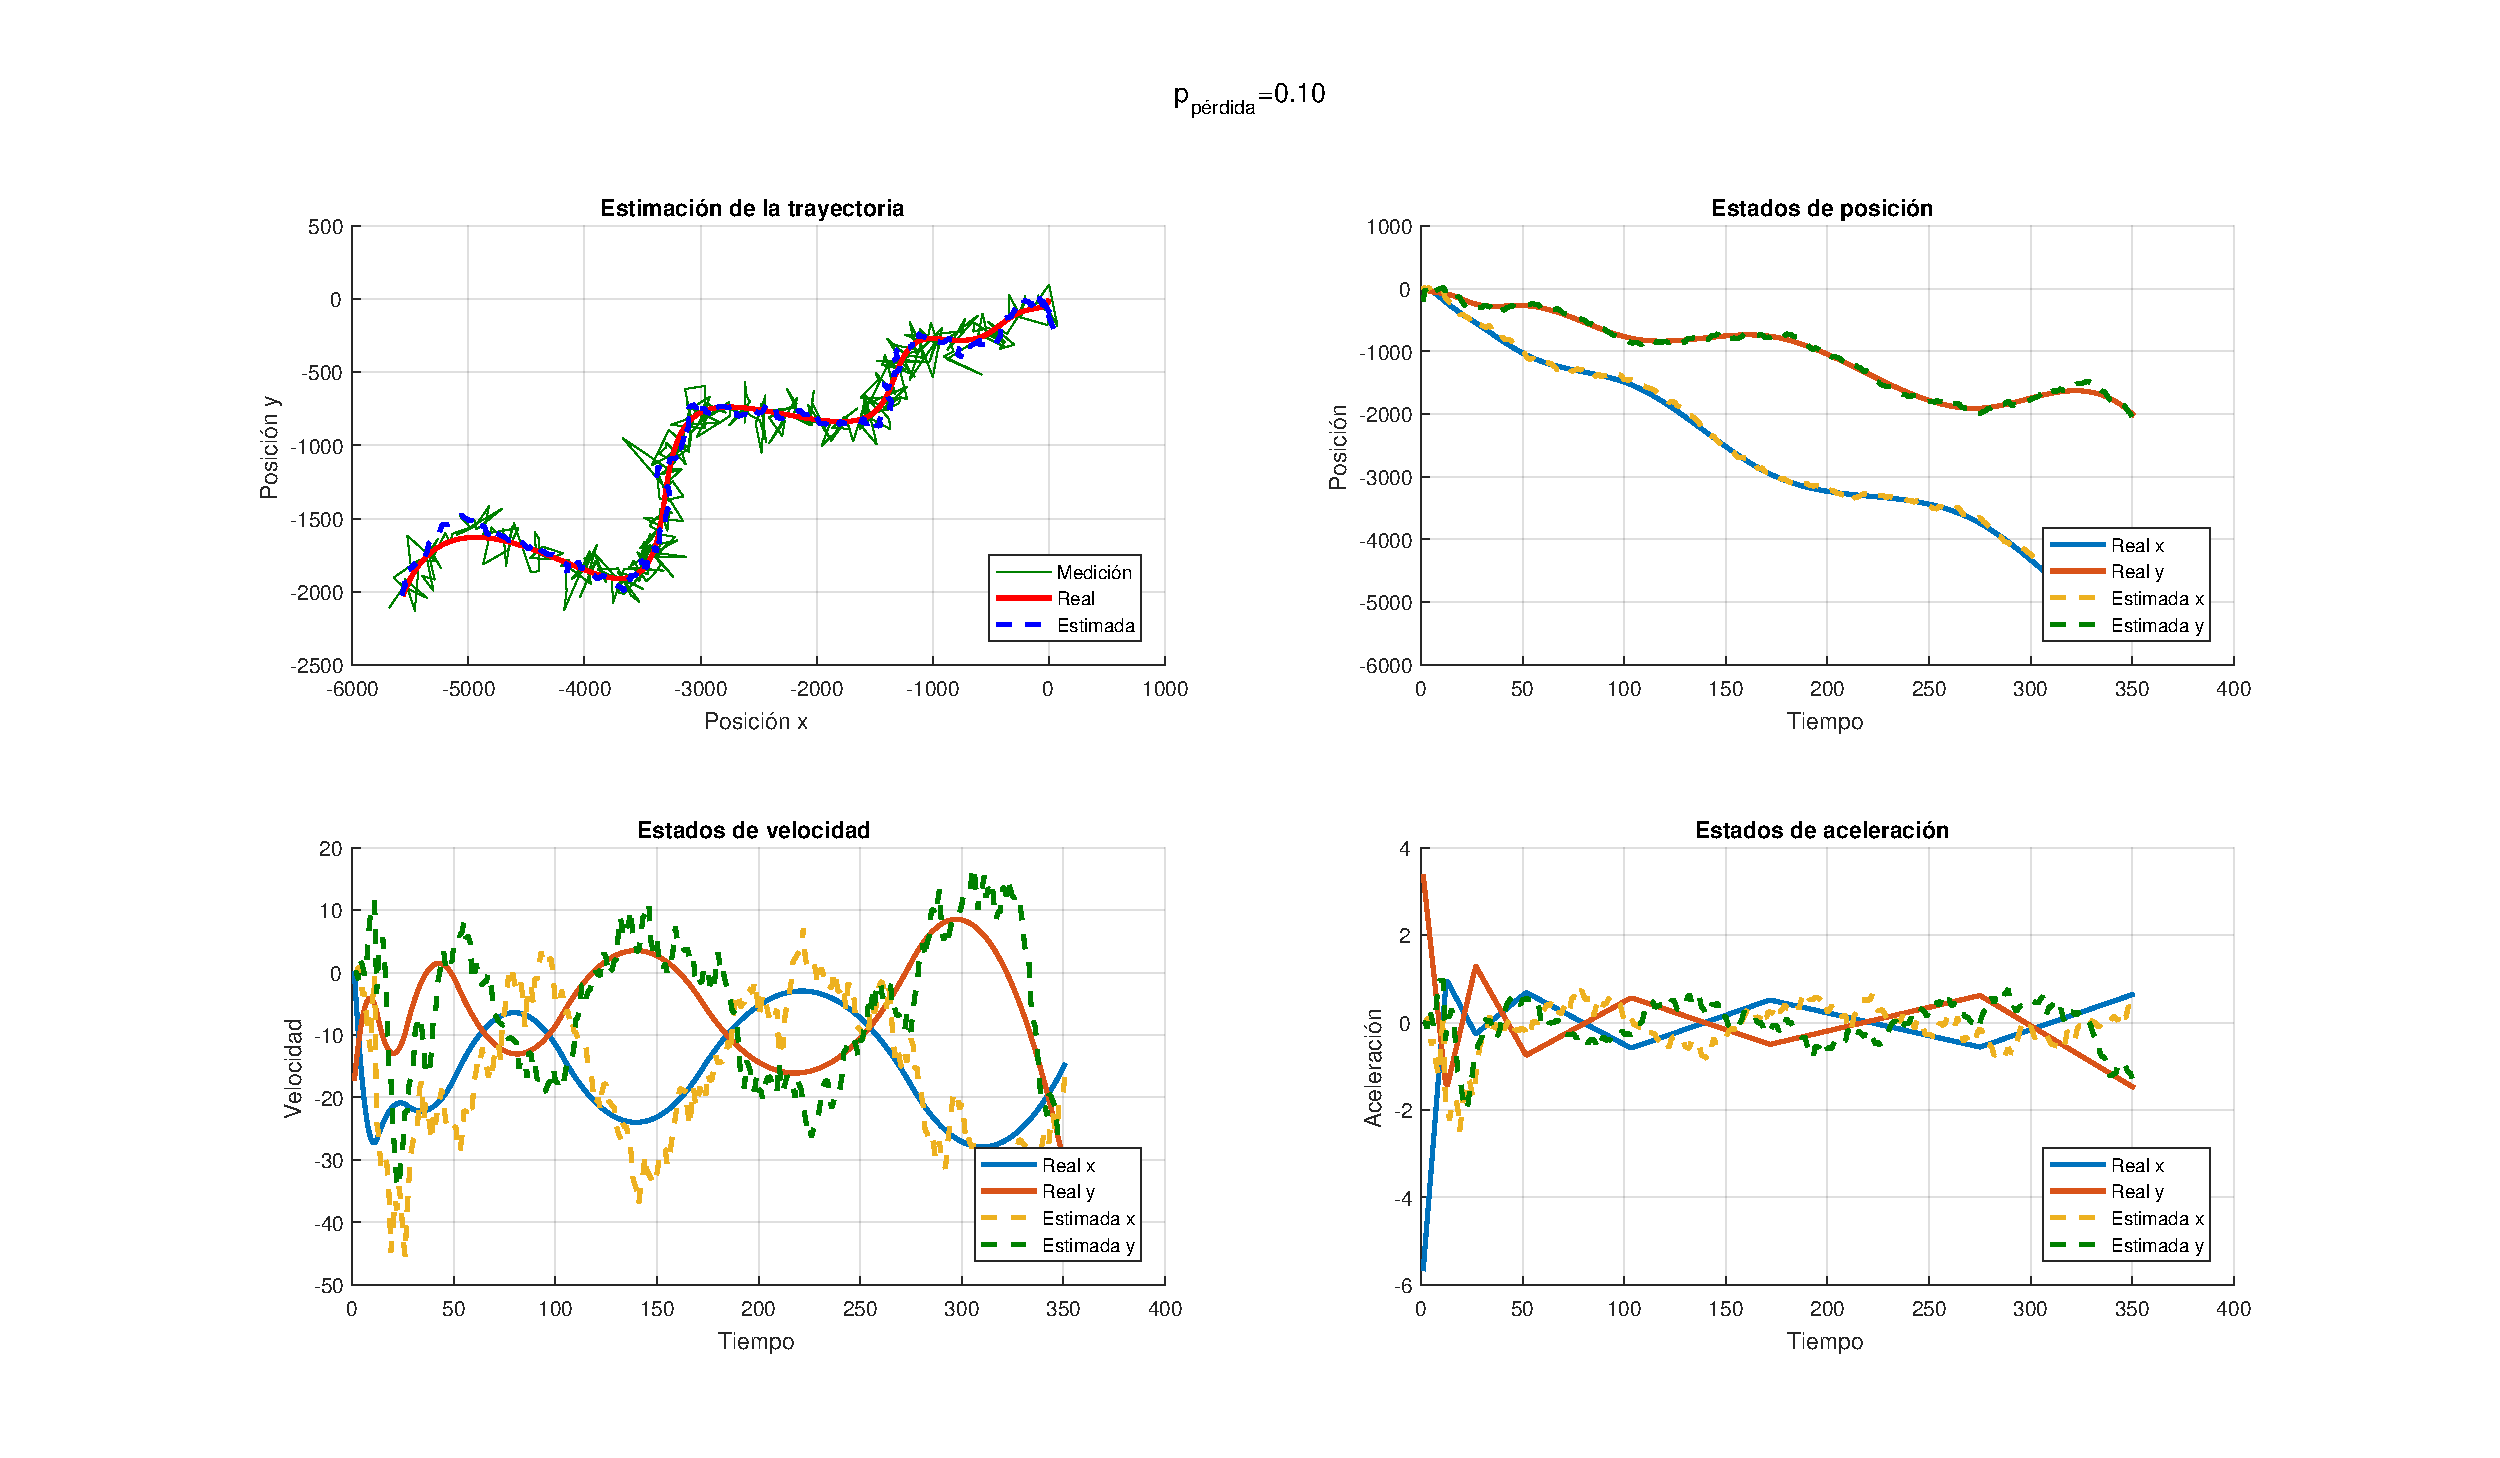
\includegraphics[scale=0.5,trim={6,5cm 0 0 0}]{Figuras/graf_ej7_1.pdf}
		\caption{Estimación De Trayectoria - Perdida Del 10 \%}
		\label{fig:ej7_1}
	\end{figure}
	
	\begin{figure}[H]
		\centering
		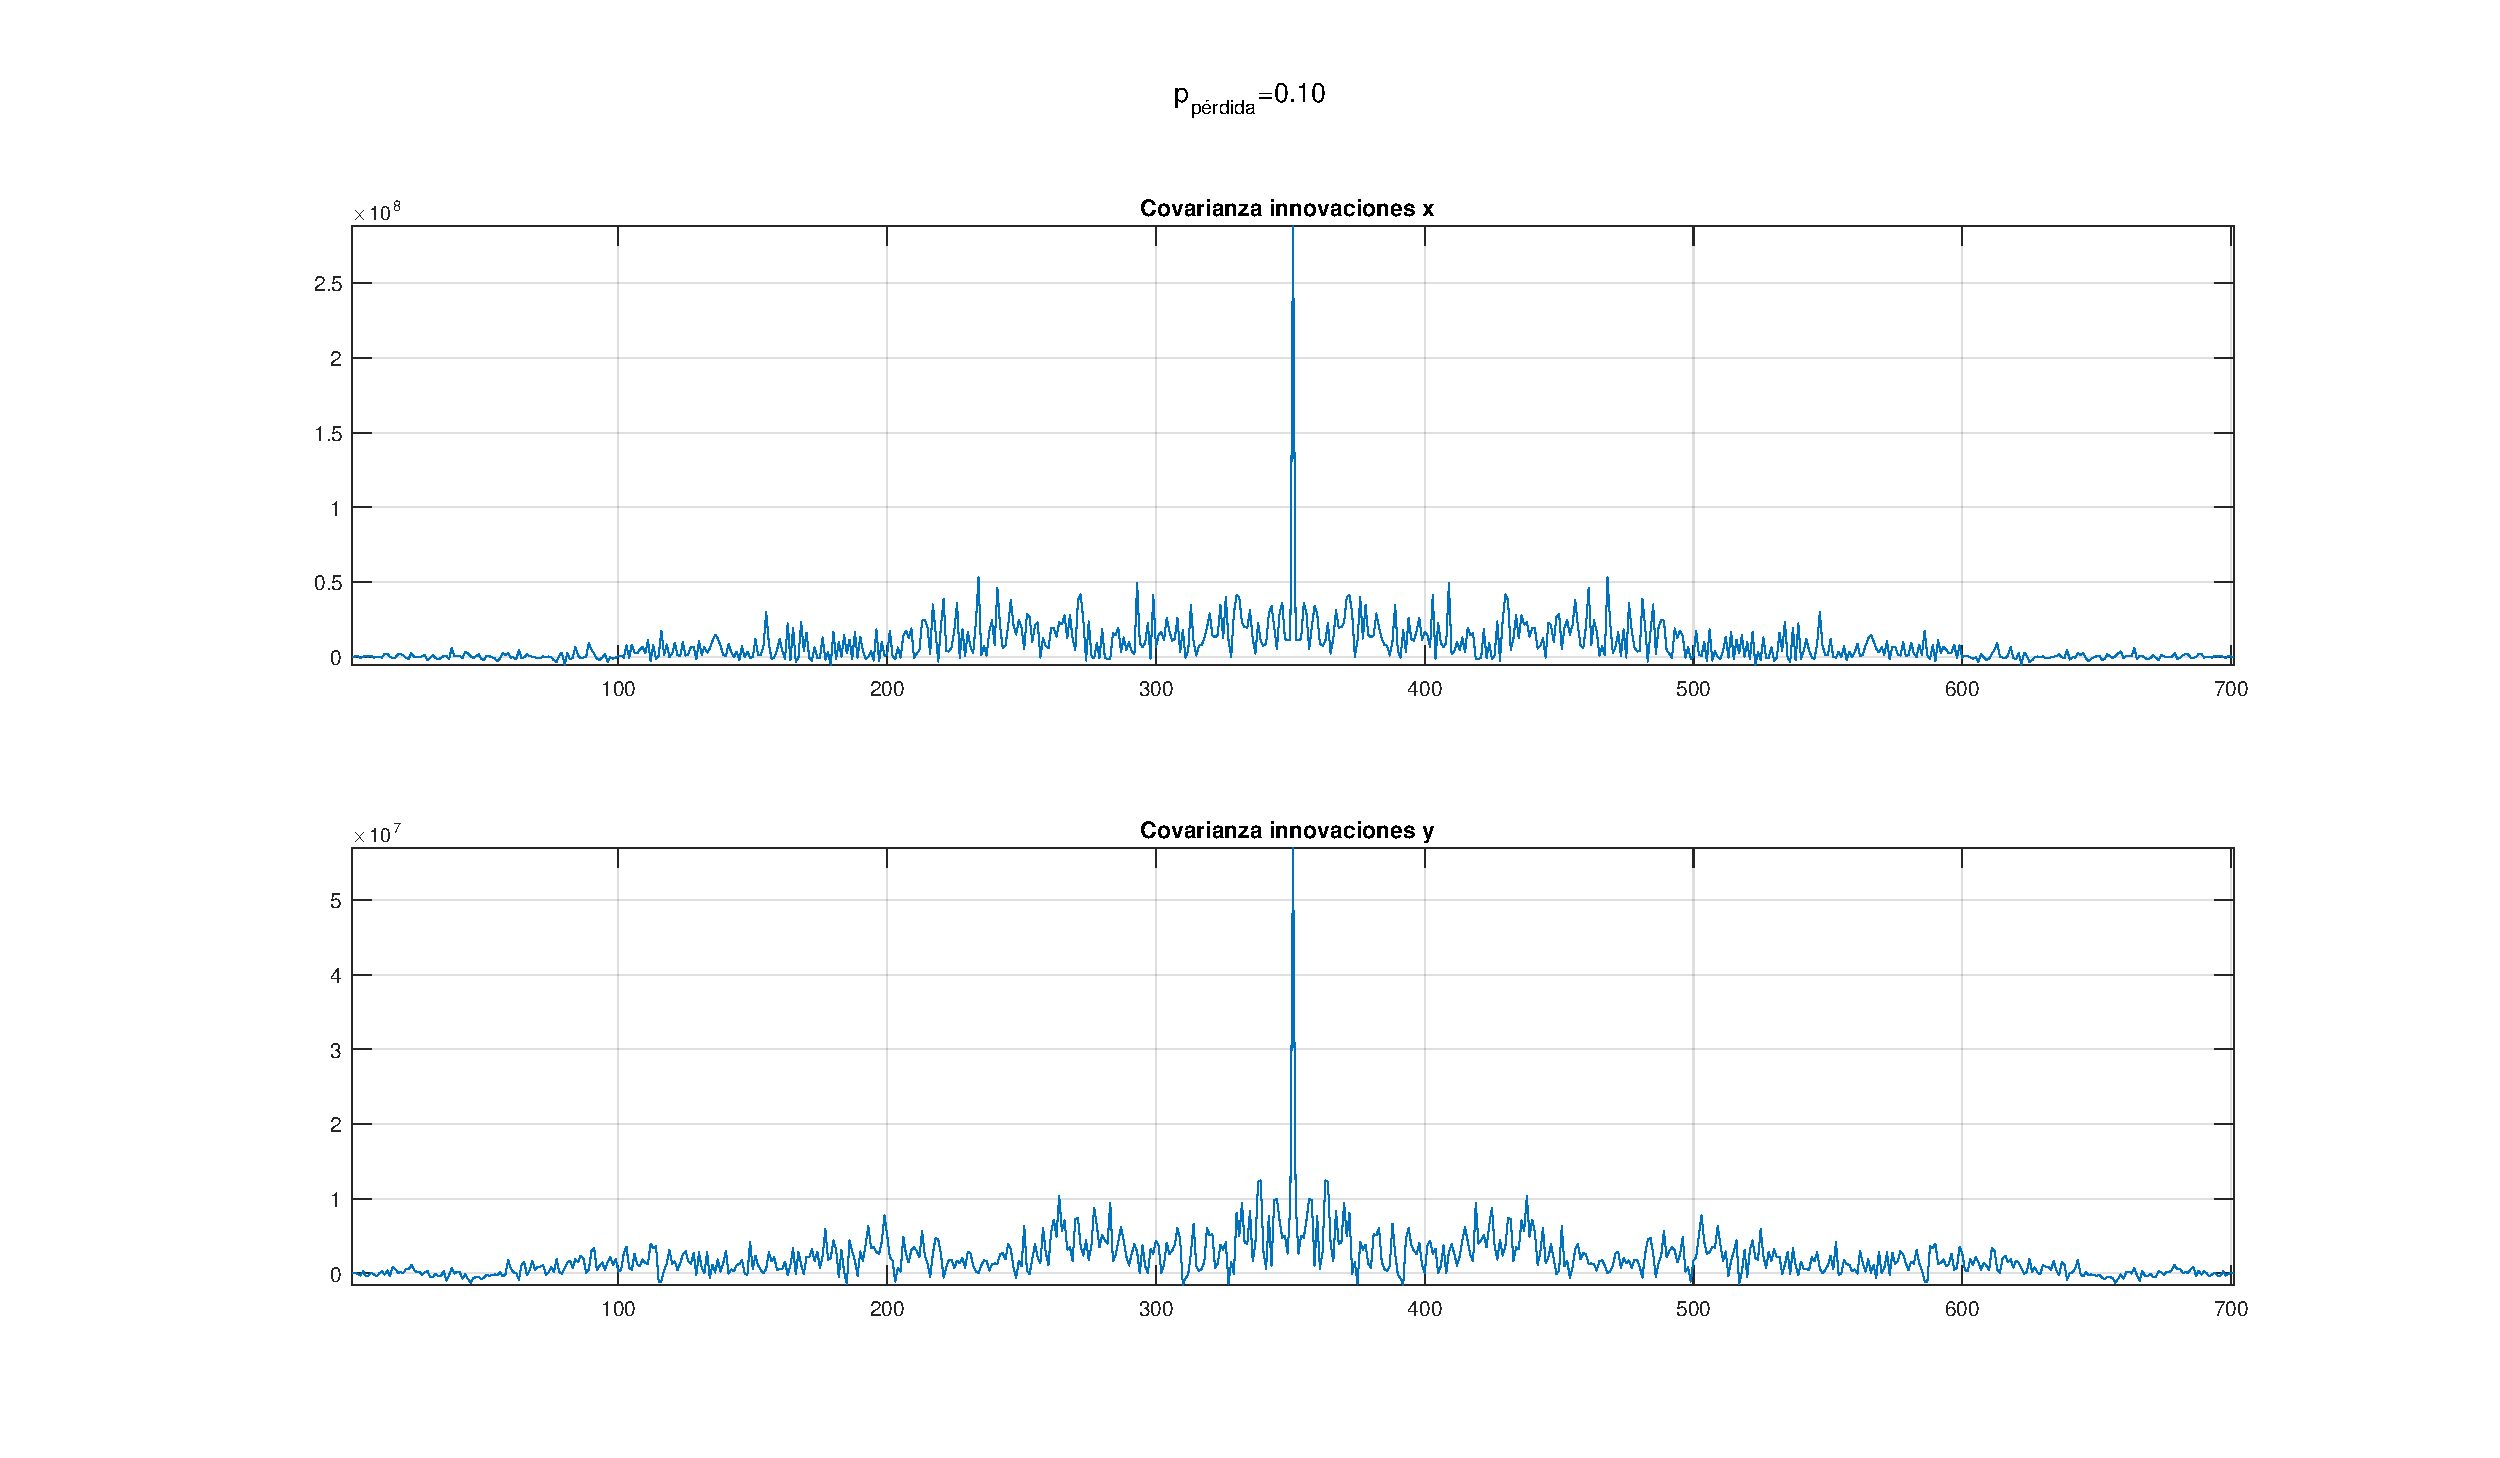
\includegraphics[scale=0.5,trim={6,5cm 0 0 0}]{Figuras/covinn_ej7_1.pdf}
%		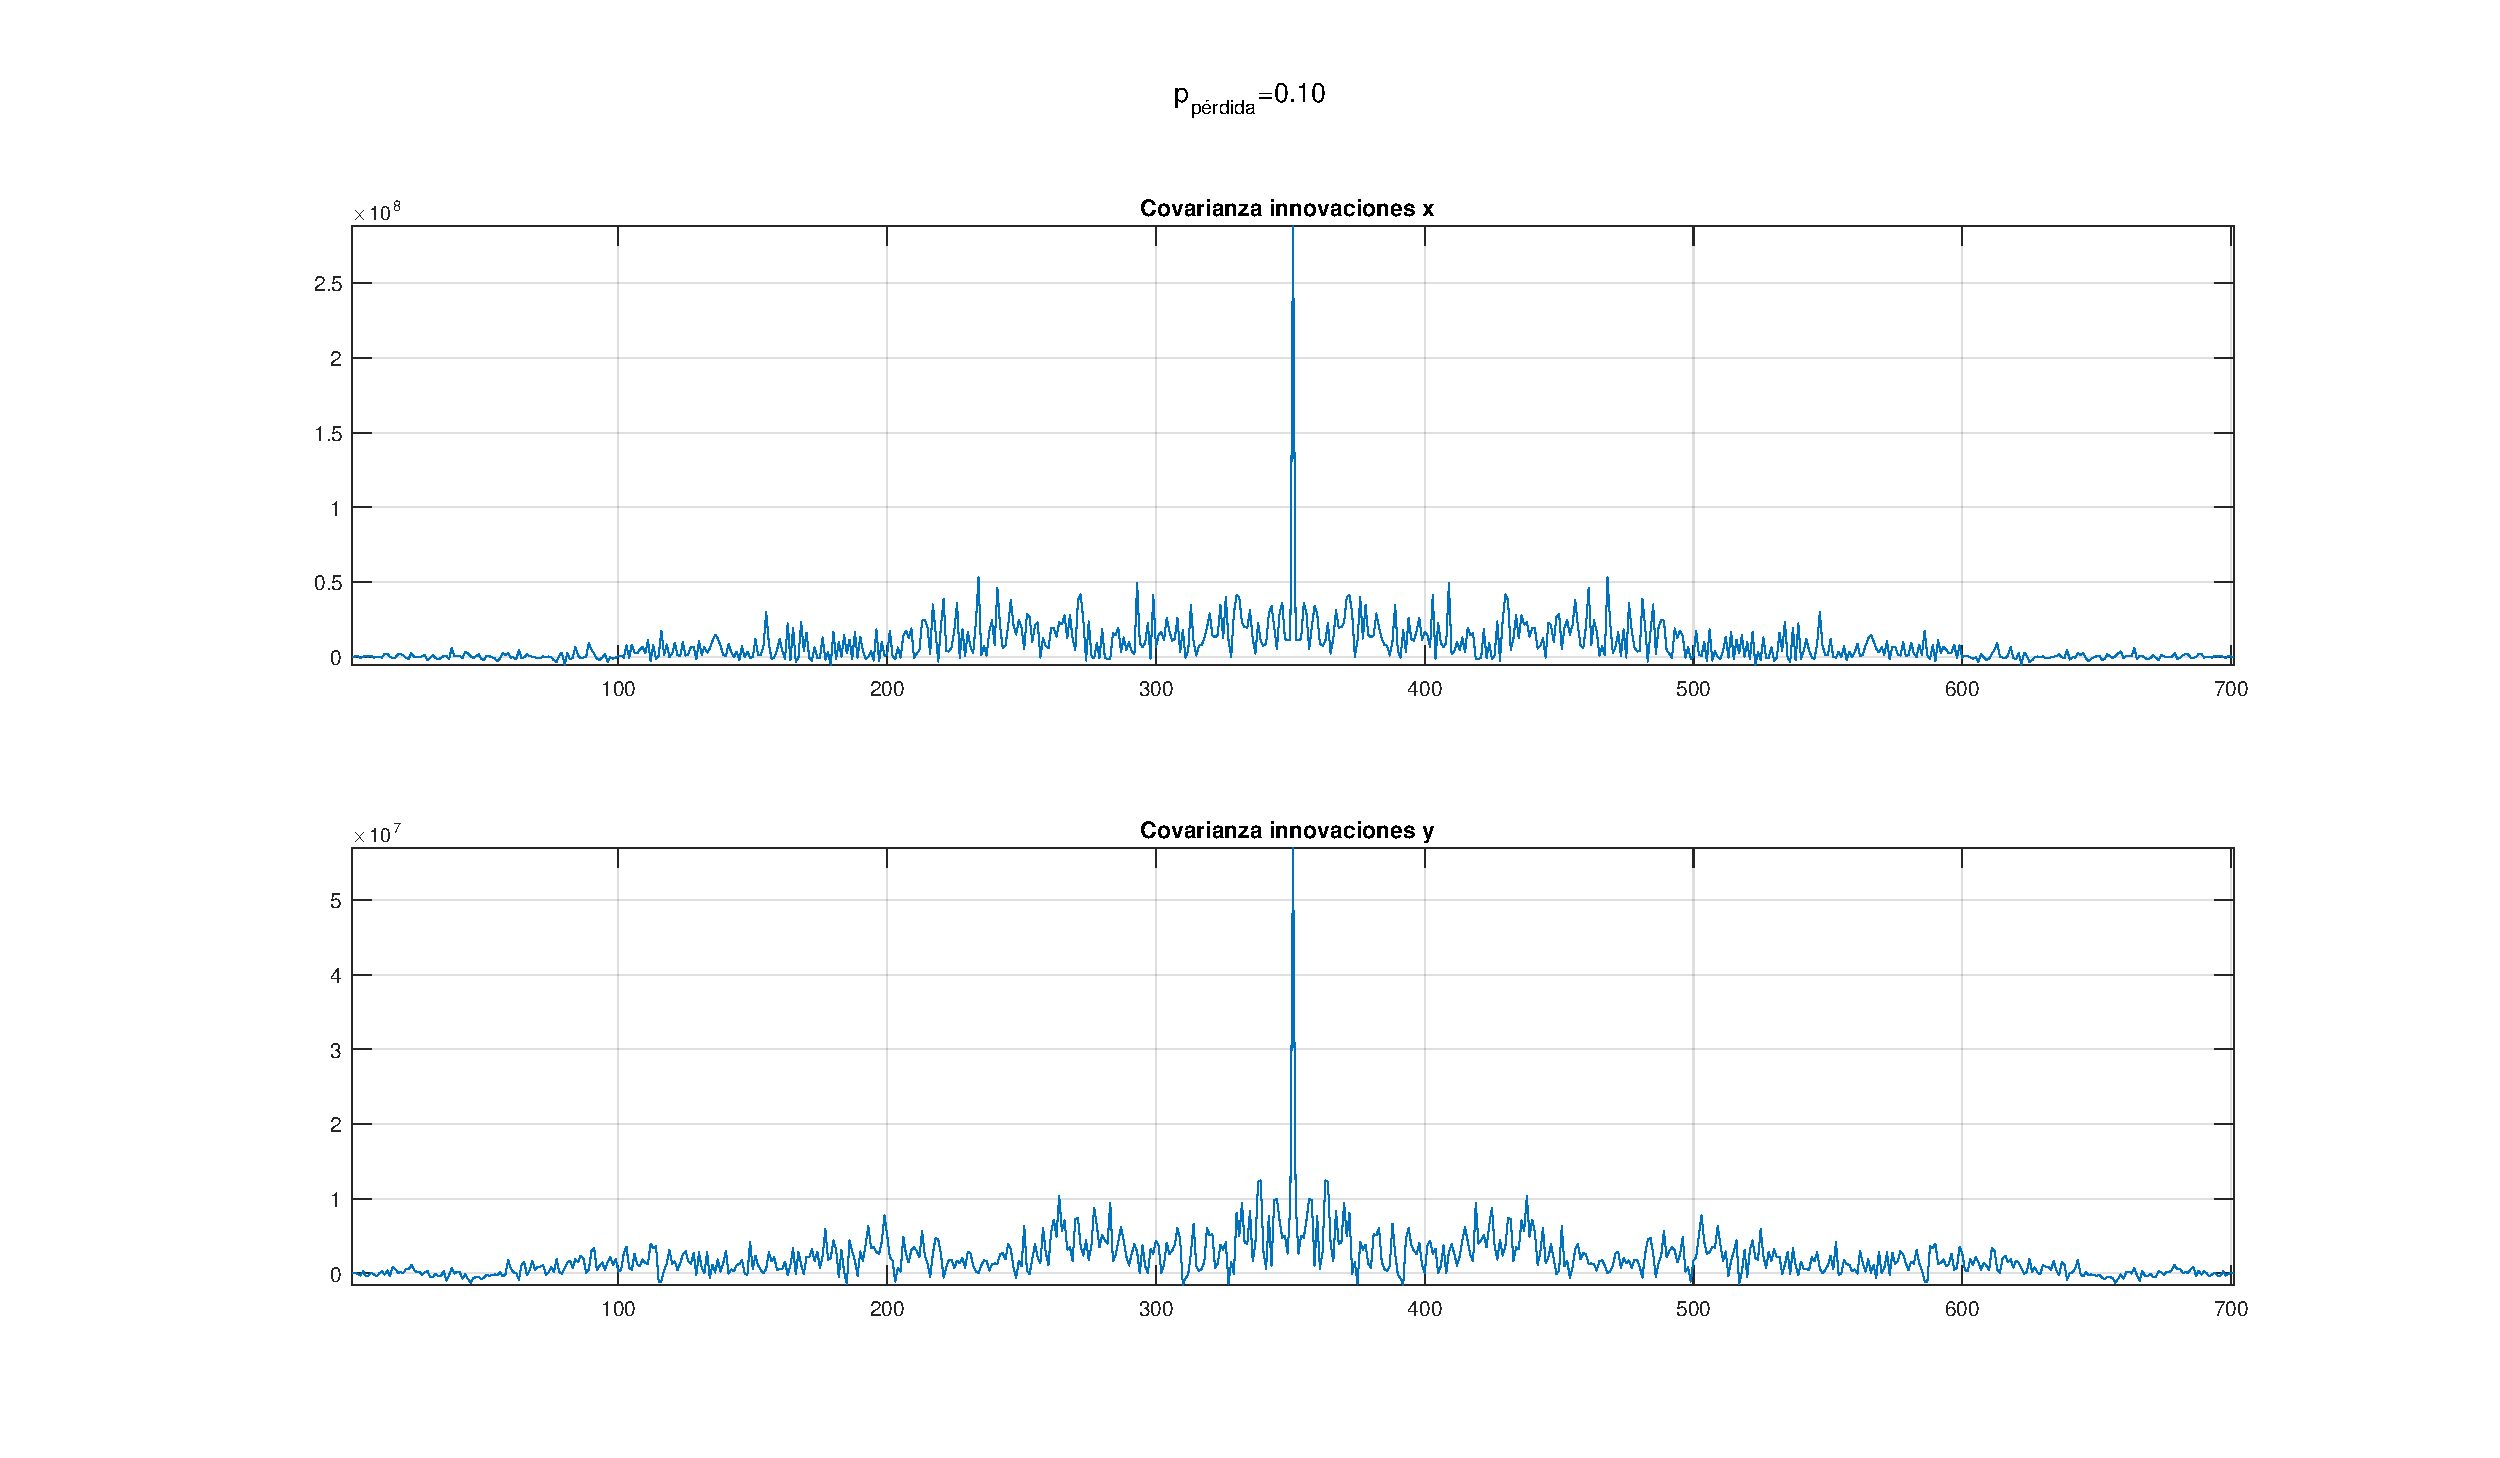
\includegraphics[width=1.0\textwidth,keepaspectratio]{Figuras/covinn_ej7_1.pdf}
		\caption{Autocorrelación De Innovaciones - Perdida Del 10 \%}
		\label{fig:ej7_1_inov}
	\end{figure}
	
	\subsection{90\% de pérdida}
	\begin{figure}[H]
		\centering
		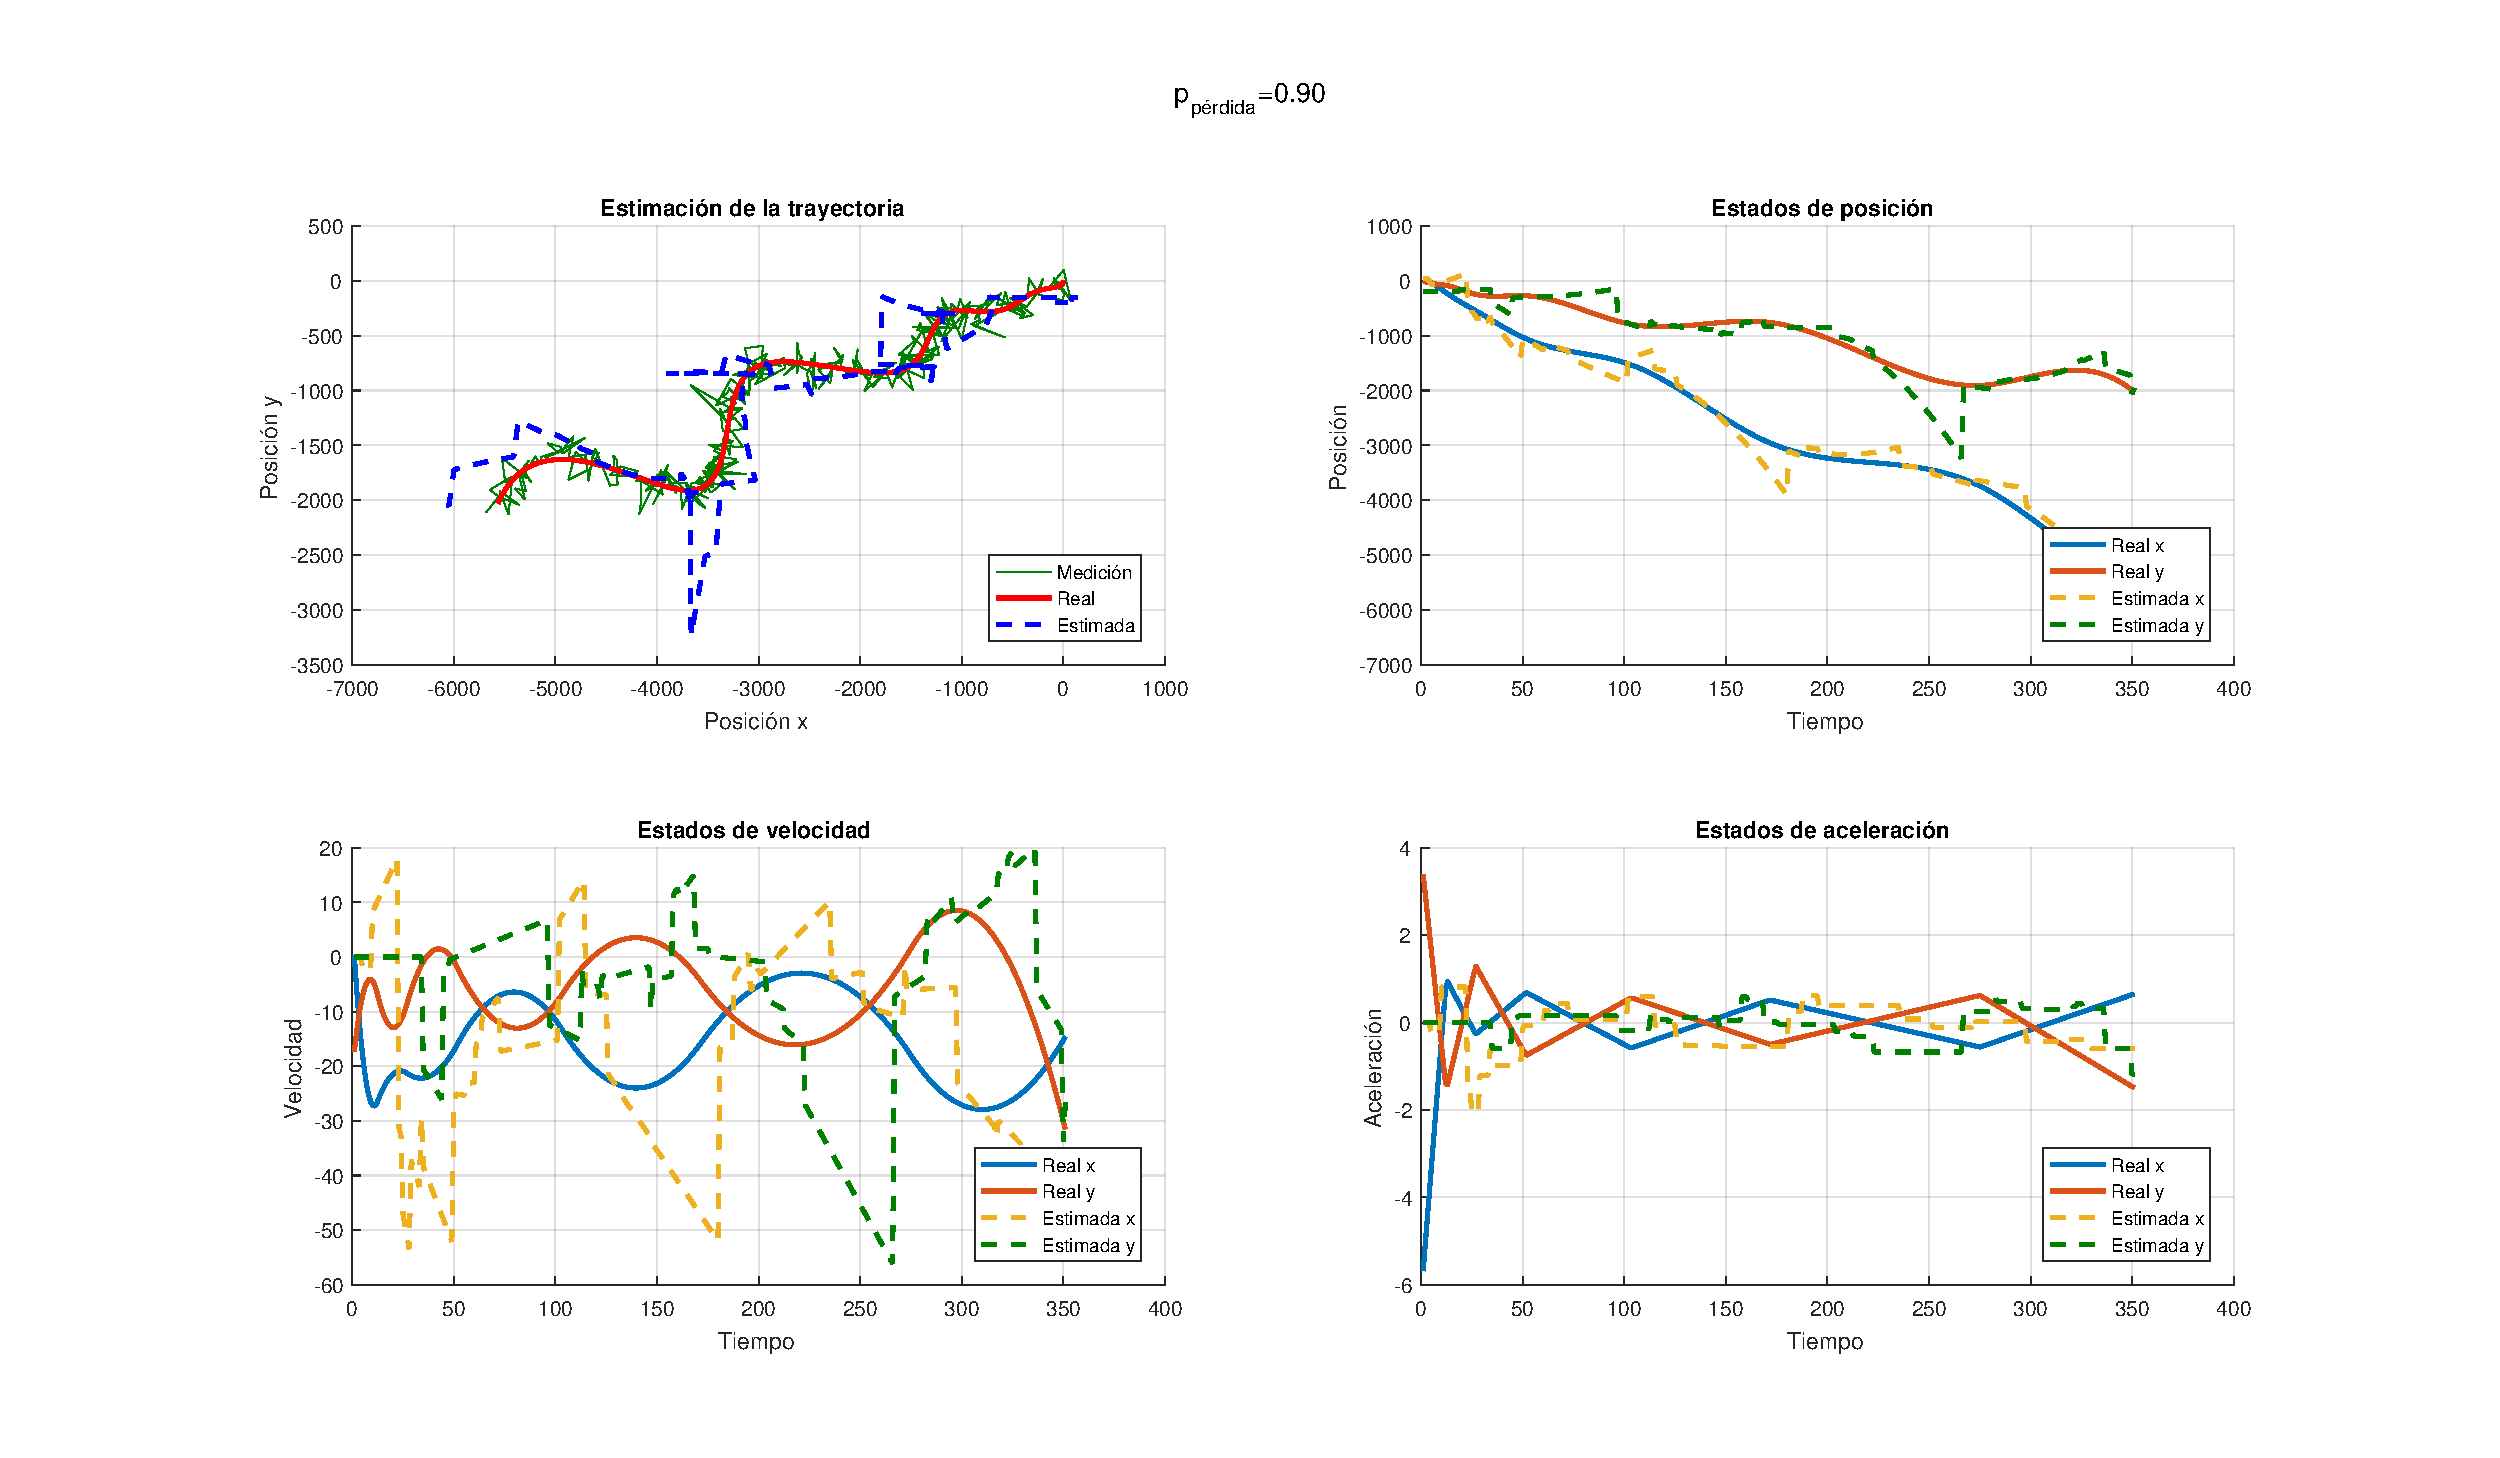
\includegraphics[scale=0.5,trim={6,5cm 0 0 0}]{Figuras/graf_ej7_2.pdf}
		\caption{Estimación De Trayectoria - Perdida Del 90 \%}
		\label{fig:ej7_2}
	\end{figure}

	\begin{figure}[H]
		\centering
		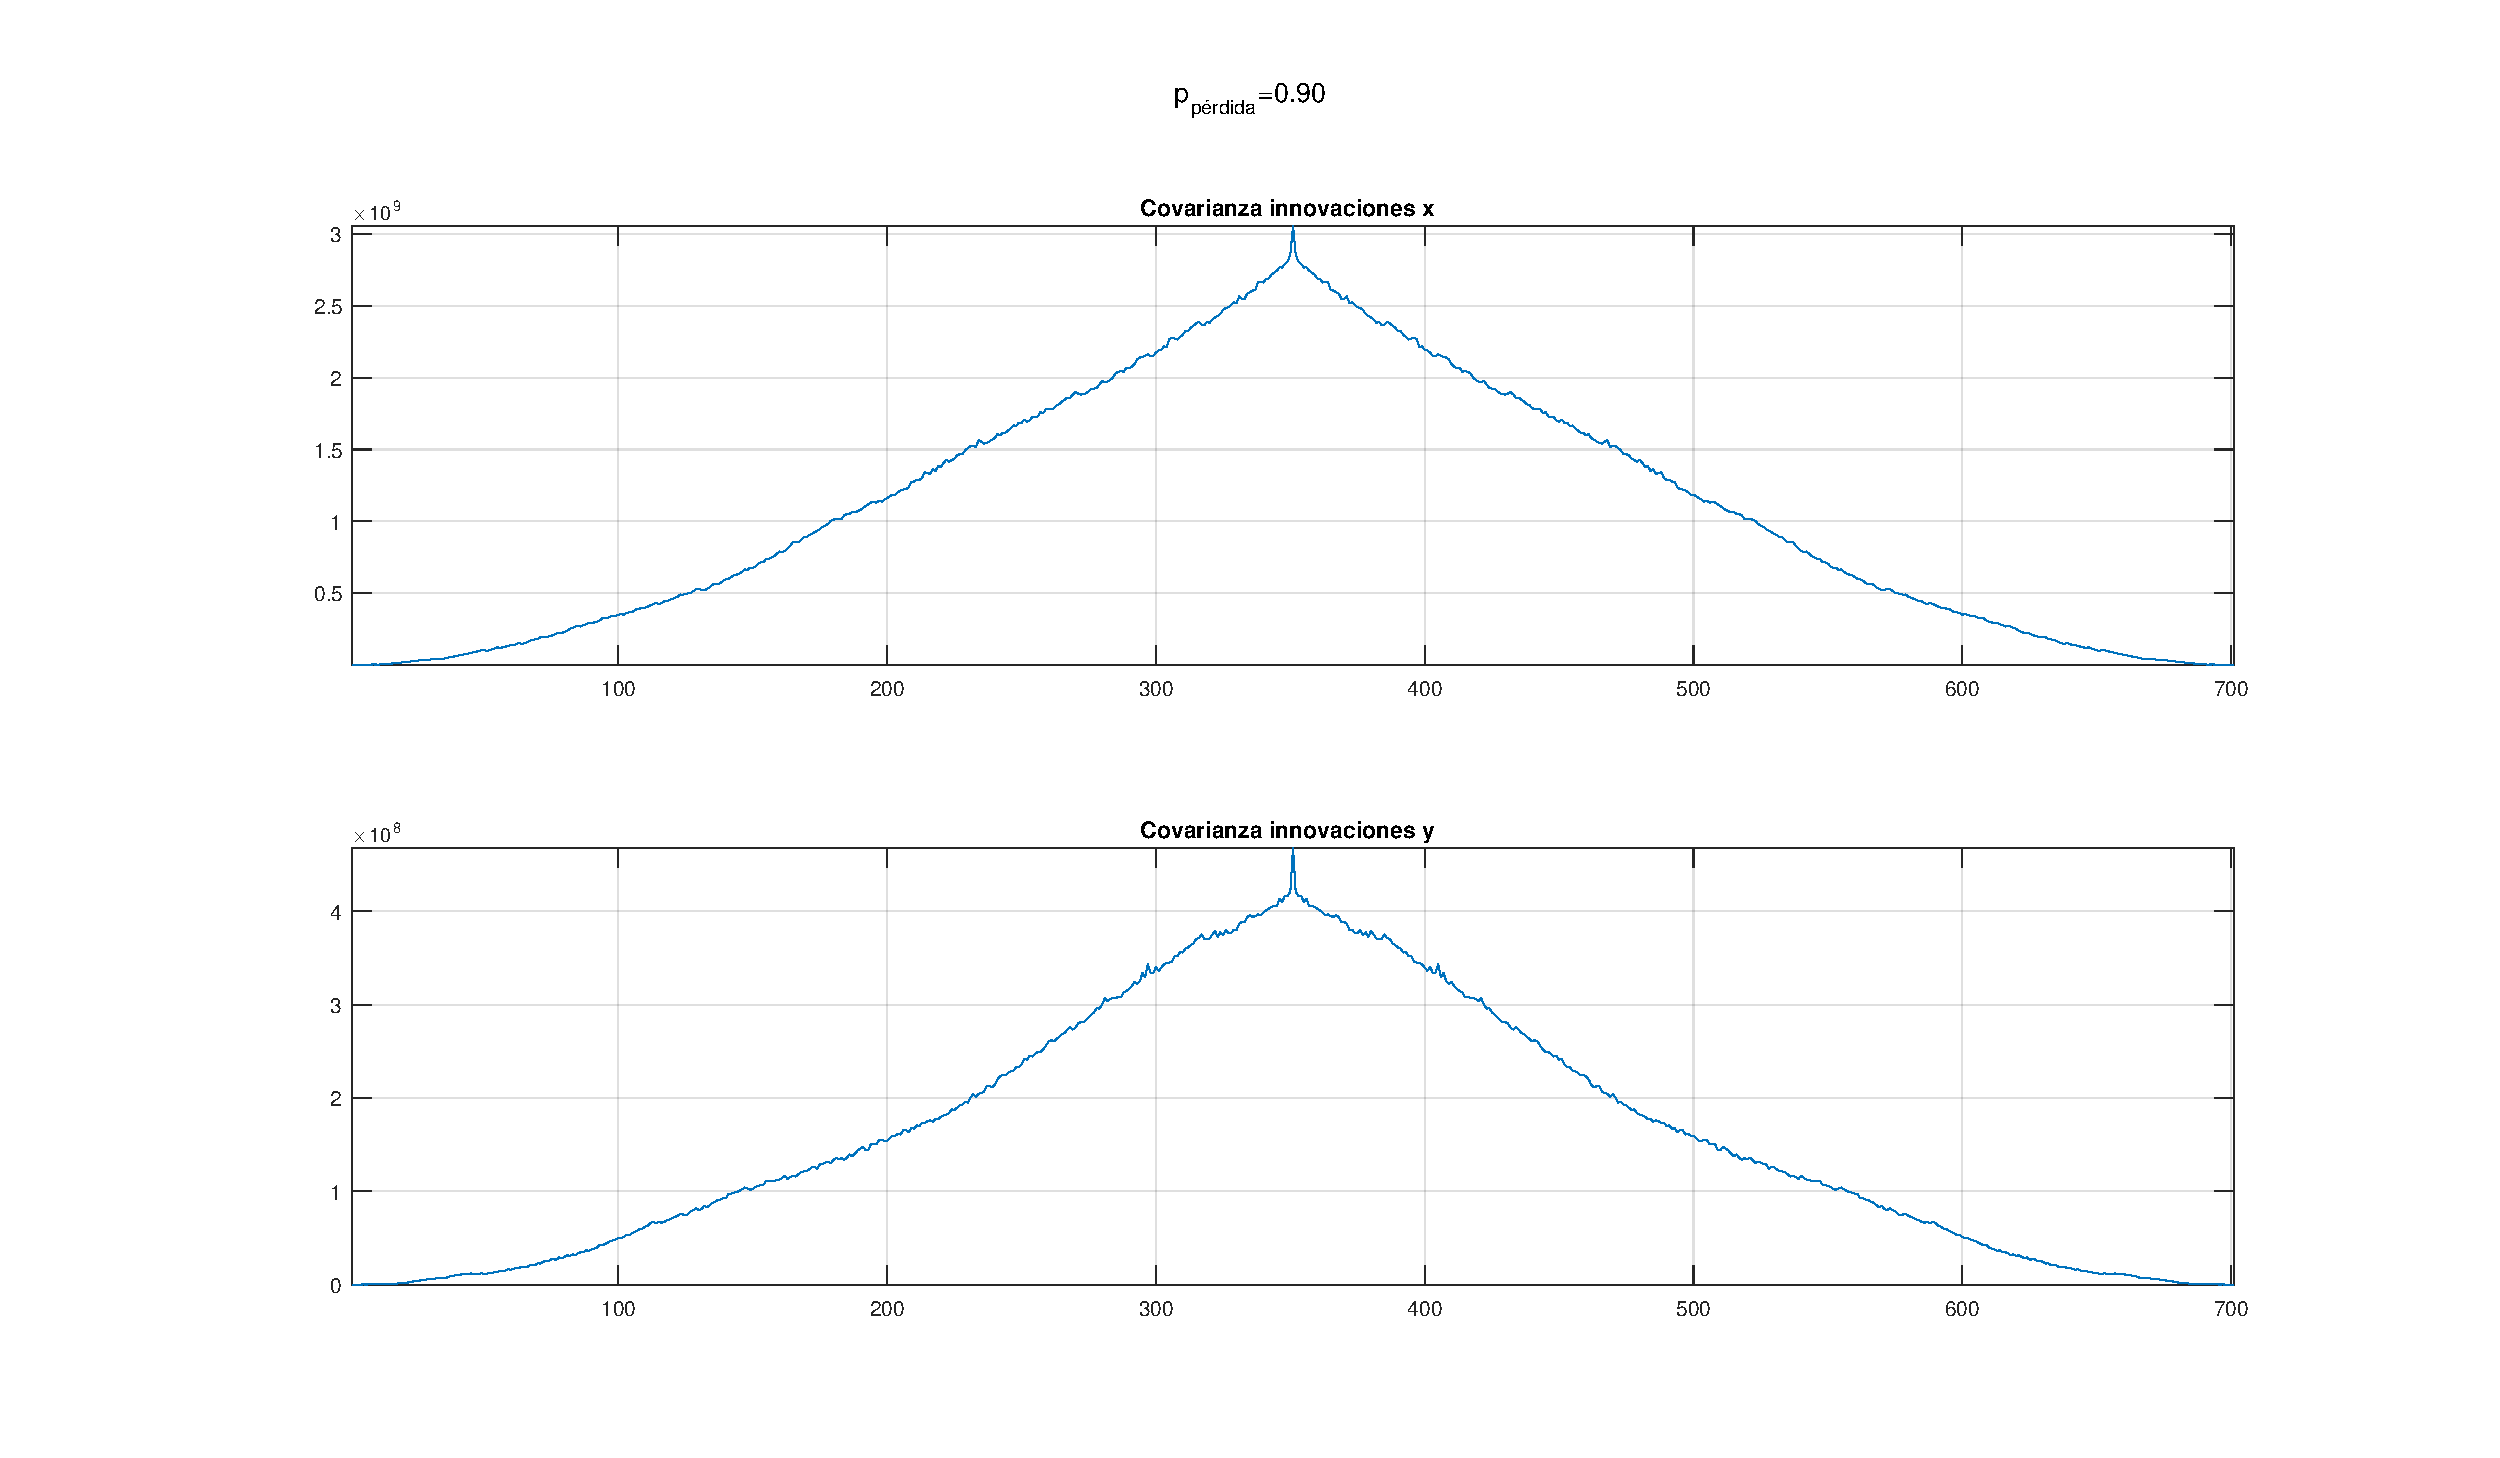
\includegraphics[scale=0.5,trim={6,5cm 0 0 0}]{Figuras/covinn_ej7_2.pdf}
%		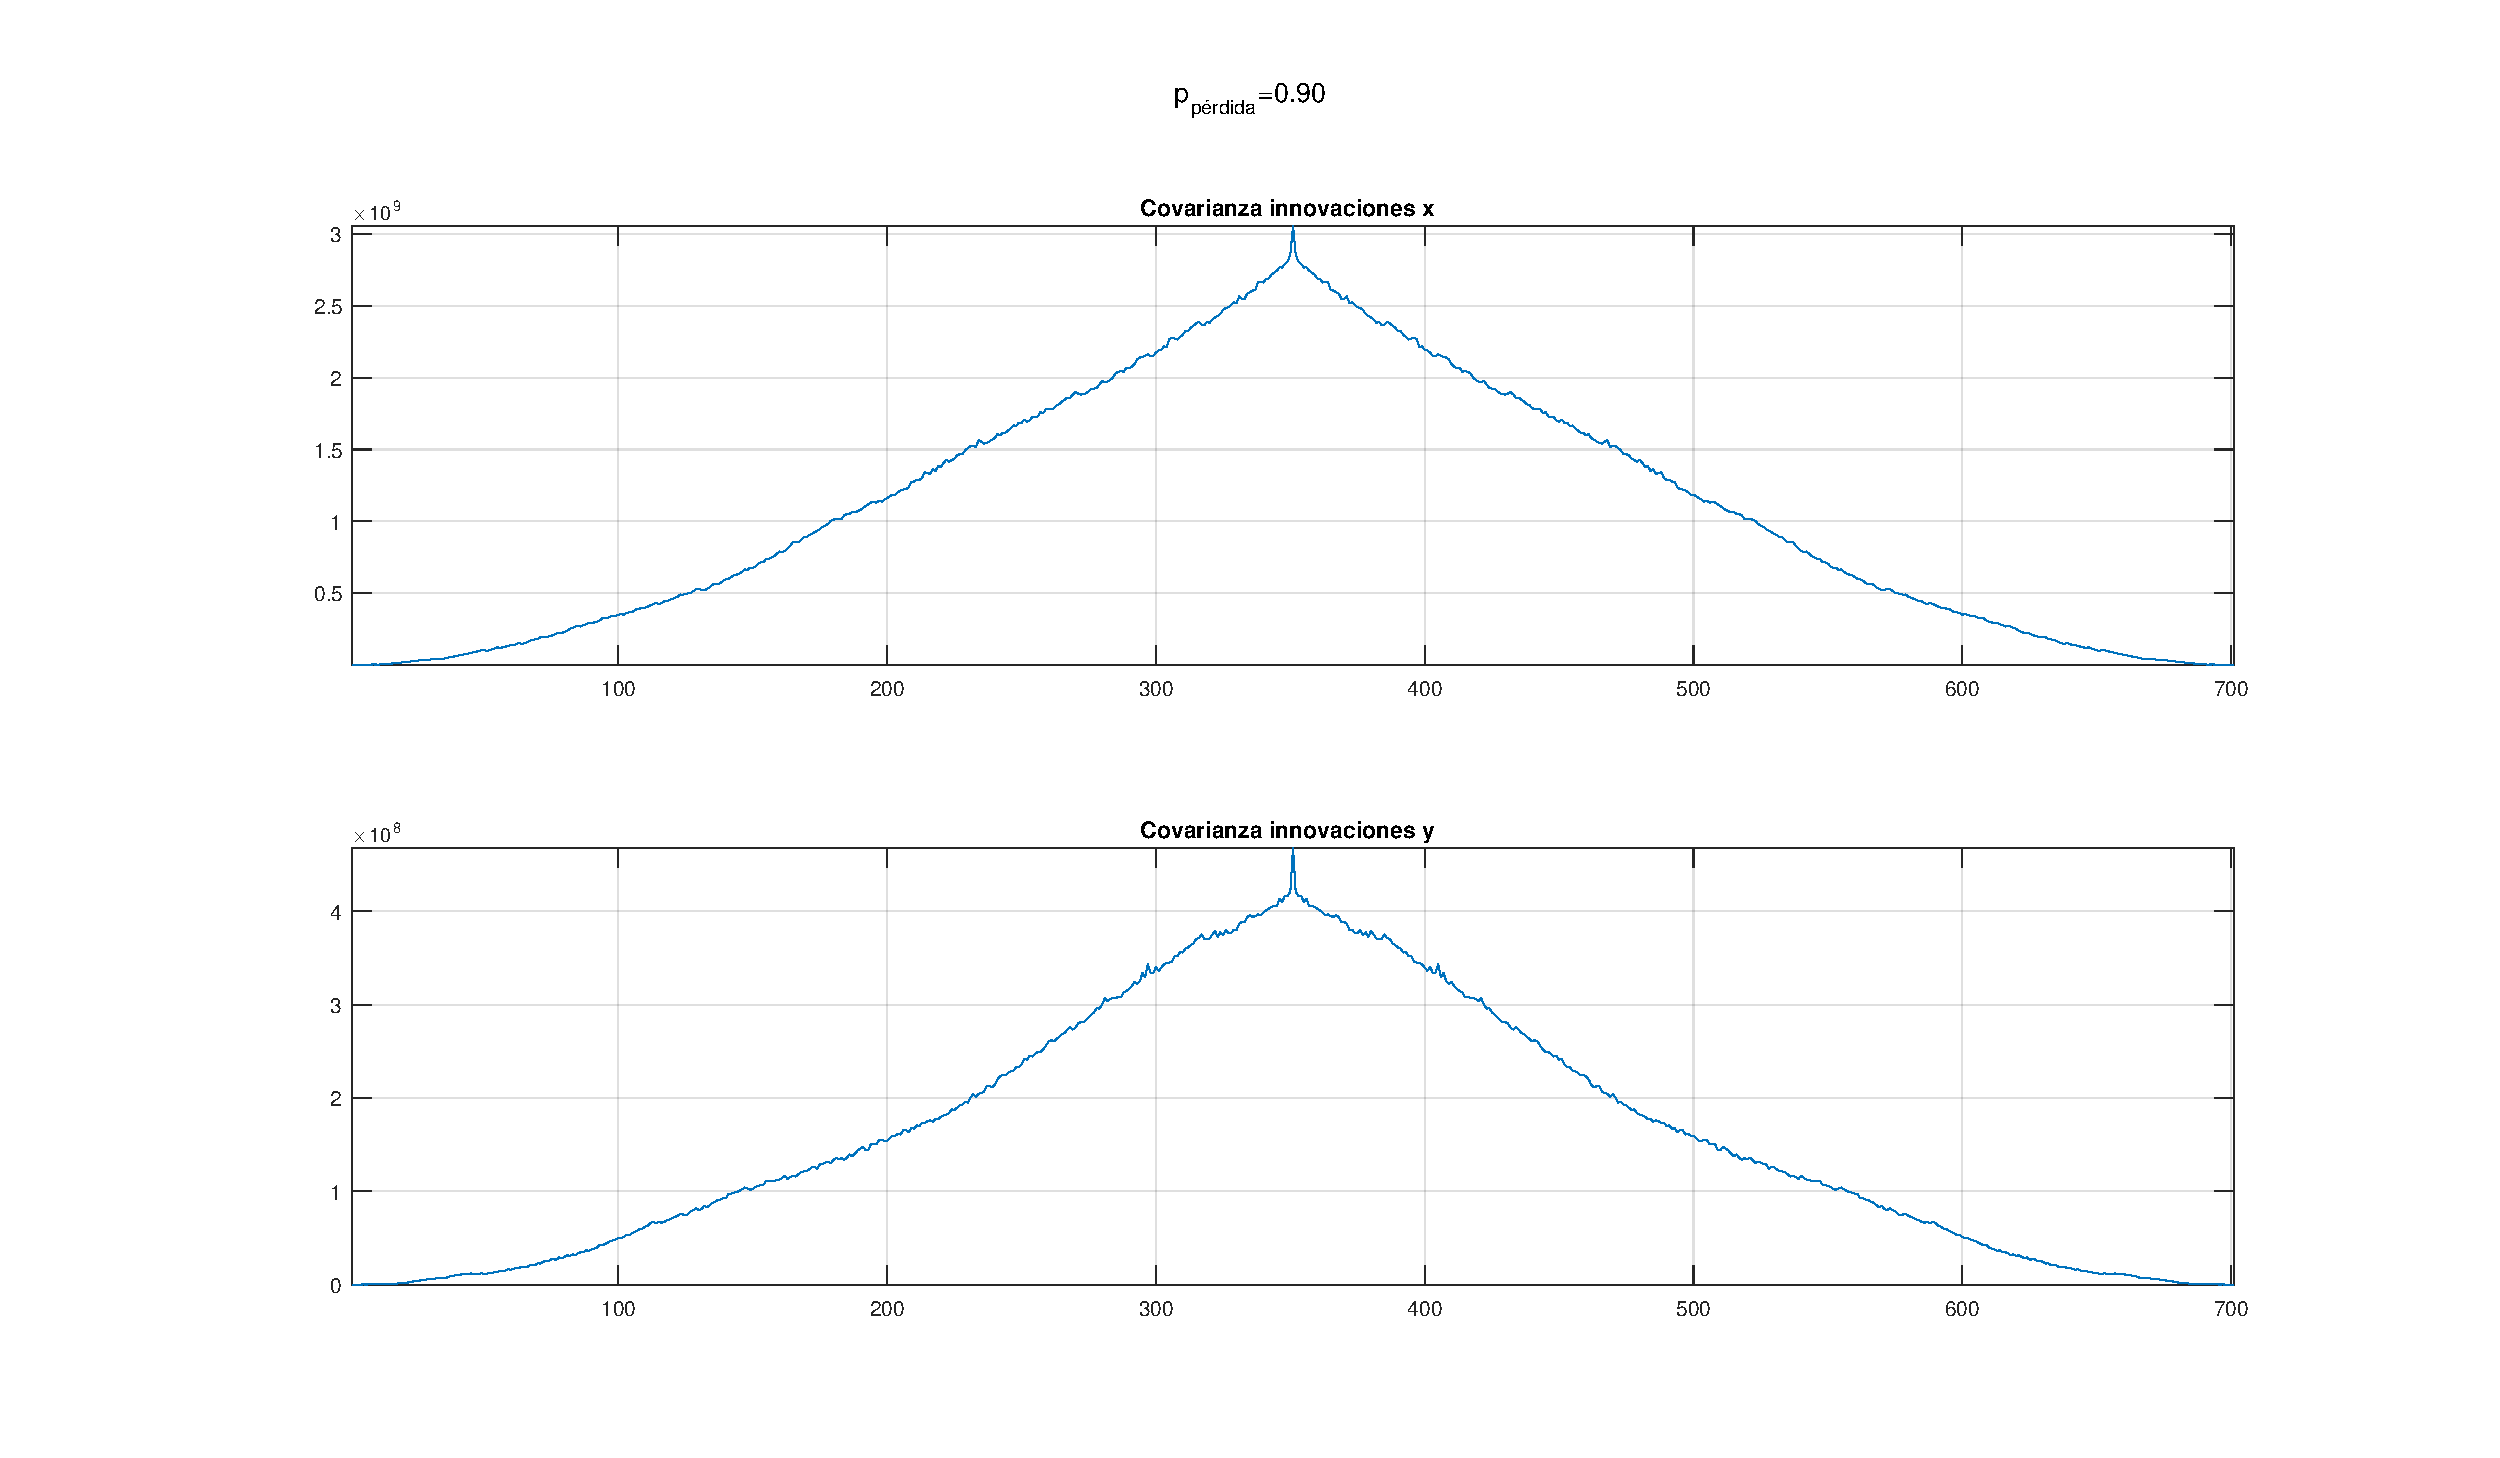
\includegraphics[width=1.0\textwidth,keepaspectratio]{Figuras/covinn_ej7_2.pdf}
		\caption{Autocorrelación De Innovaciones - Perdida Del 90 \%}
		\label{fig:ej7_1_inov}
	\end{figure}
	
	\subsection{Análisis de los resultados}

	En la Figura \ref{fig:ej7_1} puede verse lo que sucede si se pierden un 10 \% de las mediciones. En este caso el error de estimación no es severo. Por otro lado en la Figura \ref{fig:ej7_2} se observa lo que sucede cuando se pierden un 90 \% de las mediciones. Si el filtro deja de recibir información de los sensores continuará estimando con la dinámica del sistema. En el segundo caso se observa que cada vez que ocurren largos lapsos en los que no recibe mediciones el error de estimación crece cada vez más, hasta que se recibe una nueva medición que lo vuelve a colocar en la trayectoria.
	En las Figuras \ref{fig:ej7_1_inov} y \ref{fig:ej7_1_inov} se puede ver la autocorrelación de las innovaciones. Cuanto más se parezcan a ruido blanco, mejor es la estimación. Es decir, todo lo que no puede predecir el filtro corresponde a ruido blanco. También resulta notable que cuantas menos mediciones se tiene, menos se da esta propiedad.
	


	\subsection{Script}

	Para la implementación de la pérdida de datos, se modificó la iteración principal del algoritmo de Kalman. Dicha implementación se presenta a continuación.\\	
	\lstinputlisting[firstline=118, firstnumber=118, lastline=141]{../Octave/EJ7.m}


	\section{Conclusiones}\label{sec:conclusiones}
		
	\paragraph{}
	Puede sacarse como conclusión de este trabajo que el filtro de Kalman funciona muy bien a la hora de corregir el error introducido por las fuentes de ruido. Además, es bastante versátil ya que permite incorporar y resumir información de varias fuentes de mediciones a la vez. Sin embargo, hay una fuerte dependencia de los resultados con la observabilidad. Se vio que en muchos casos la misma es un factor limitante importante.
	
	\paragraph{}
	Por otro lado, la técnica funciona bien cuando los ruidos son de media nula. Si la media de los ruidos de mediciones es desconocida y no nula, la técnica de incluirla como un estado a estimar tiene sus limitaciones, como ya se dijo, ligadas a la observabilidad. De los casos vistos, son pocos en los que se puede estimar las medias en forma satisfactoria.
	
	\paragraph{}
	Se comprobó además el funcionamiento del algoritmo cuando no se puede hacer una buena estadística del estado inicial. Si no se conoce el mismo o su media con certeza, basta con indicarle en la matriz $P$ que el dato es poco confiable para que el algoritmo procese y converja debidamente a la trayectoria.
	
	\paragraph{}
	El algoritmo basado en usar las matrices estacionarias en lugar de calcular la ganancia de Kalman instante a instante funciona razonablemente bien en comparación con el algoritmo original. Bastó con un corto intervalo de tiempo para que la trayectoria siguiera a la original, y además el algoritmo modificado posee la misma inmunidad al ruido que el original.
	
	\paragraph{}
	La variante del algoritmo de Kalman con pérdida de datos, modificando la matriz $C$, es una herramienta muy útil ya que no todo el tiempo se tienen mediciones de todos los sensores. Contar con un algoritmo que realice una síntesis de datos que llegan de varios sensores, en tiempos diferentes, es de suma utilidad práctica. La posibilidad de poder modificar la matriz $C$ instante a instante está ligada a otra ventaja del filtro de Kalman poco explorada en el trabajo que es la posibilidad de tratar con sistemas variantes en el tiempo.
	
	\paragraph{}
	En resumen, el filtro de Kalman es de suma importancia práctica dado que se comporta bien en situaciones más reales que ideales. En ellas los factores condicionantes son: trabajar con sistemas que varian en el tiempo (aunque en este trabajo no se exploró en profundidad esta ventaja), trabajar con señales en presencia de ruido, y sintetizar información de distintos sensores que miden diferentes cosas, y con errores distintos, en un único resultado a la salida del algoritmo.


	% \appendix
\end{document}
